\documentclass[]{report}
\usepackage[pdftex]{hyperref, graphicx}
\usepackage[all]{hypcap}
\usepackage{url, subfigure, lscape, afterpage, float}

\date{October 2012}
\title{Ondex tutorial and user guide}
\author{contact@ondex.org}
\newcommand{\exerciserule}{\vskip 10pt \hrule \vskip 10pt}

\begin{document}

\sloppy
\maketitle
\tableofcontents

\vspace{1cm}
\emph{Revisions}
\begin{itemize}
\item{June 2012:} Chapter 1 Data visualisation
\item{October 2012:} Chapter 2 Data integration
\item{October 2012:} Chapter 3 GUI reference
\item{October 2012:} Chapter 4 How do I compare genomic data in Ondex?
\item{October 2012:} Chapter 5 How do I analyse micro-array data using Ondex?
\item{October 2012:} Chapter 6 How do I look at QTLs in Ondex?
\item{October 2012:} Chapter 7 How do I study protein-protein interactions in Ondex?
\item{October 2012:} Appendix A FAQs
\item{October 2012:} Appendix B List of accession types
\item{October 2012:} Appendix C List of relation types
\item{October 2012:} Appendix D Importing data in Ondex \footnote{only updates, no new additions}
\item{October 2012:} Appendix E Mapping data in Ondex \footnote{only updates, no new additions}
\end{itemize}

%%%%%%%%
%% Include chapter files here
%%%%%%%%
\chapter{Data visualisation}
\label{cha:visualisation}
Nodes in a network represent biological concepts ({\it{e.g.}} genes / proteins / metabolites) and biological interactions are modeled as links between them, {\it{i.e.}} relations between concepts ({\it{e.g.}} a gene encodes a protein).
Firstly, we will look at the basic user interface of Ondex.
Then we will load up a network to show the commonly used features and some of the core functionality such as layouts, annotators and filters. 

Help on starting Ondex is available in Section \ref{sec:ref_install}.
Once launched, you should see a window that looks like in Figure \ref{fig:launch_Ondex}.

\begin{figure}[H]
\centering
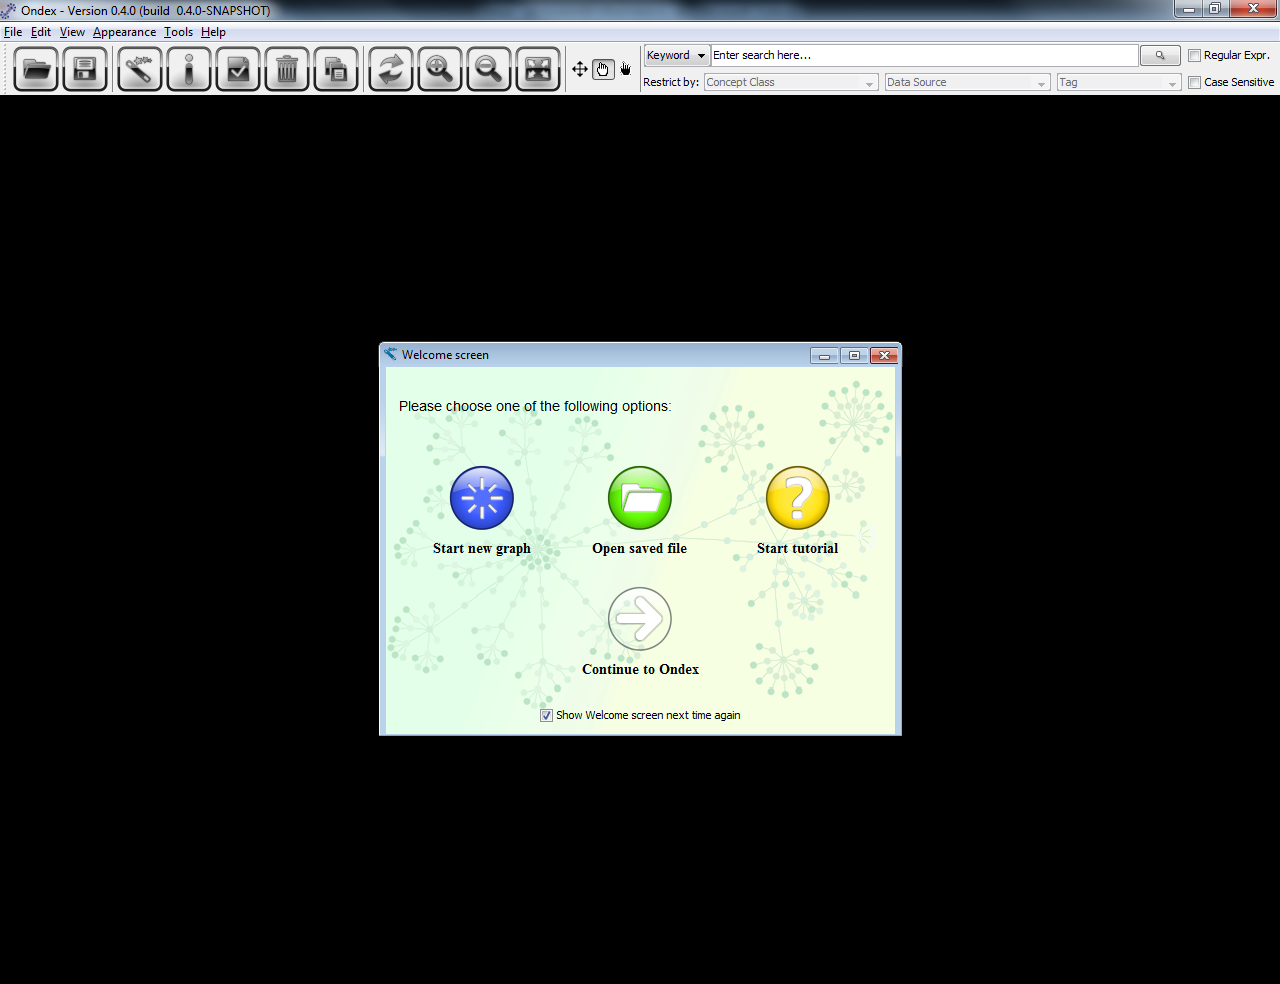
\includegraphics[scale=0.3]{images/Jun12/launched_Ondex.png}
\caption{Launching Ondex}
\label{fig:launch_Ondex}
\end{figure}

\begin{itemize}
\item At the top of the Ondex window there is a tool-bar which contains the menus, icons and search bar. 
Tool-tips are available for each icon when the mouse pointer hovers over it.
\item The rest of the window is used to show visualisation windows and pop-up dialog boxes to set up filters, annotators, etc.
\item When Ondex is launched, a welcome screen is displayed in the middle of the main window. 
This welcome screen window offers the users four buttons which are shortcuts to opening an empty network, opening an existing network, starting the tutorial or continuing to Ondex without taking any immediate action. 
Finally, at the bottom of the window, users are given the option of deselecting a check-box if they do not wish this welcome screen window to pop up automatically the next time Ondex is started.
\end{itemize}

%%%%%%%%%%%%%%%%%%%%%%%%%%%%%%%%%%%%%%%%%%%%%%%%%%%%%%%%%%%%%%%%%%%%%%%%%%%%%%%%%%%%%%%%%%%%%%%%%%%%%%%%%%%%%%%%%%%%%%%%%%%%%%%%%%%%%%%%%%%%%%%%%%%%%%%%%%
\section{Loading Networks and Basics}
\label{sec:loading}
We will now load a network (a subset of the AraCyc database) to show commonly used features of the user interface.
More information on loading and saving networks is available in Section \ref{sec:ref_loading}.
\begin{itemize}
\item Go to File -$>$ Open  (or click on the first button in the icon bar)
\item You should see an Open File Dialog
\item Open the Tutorial\_files/Main\_part folder, select aracyc\_subset.oxl and click on open
\end{itemize}
You should see the following:
\begin{figure}[H]
\centering
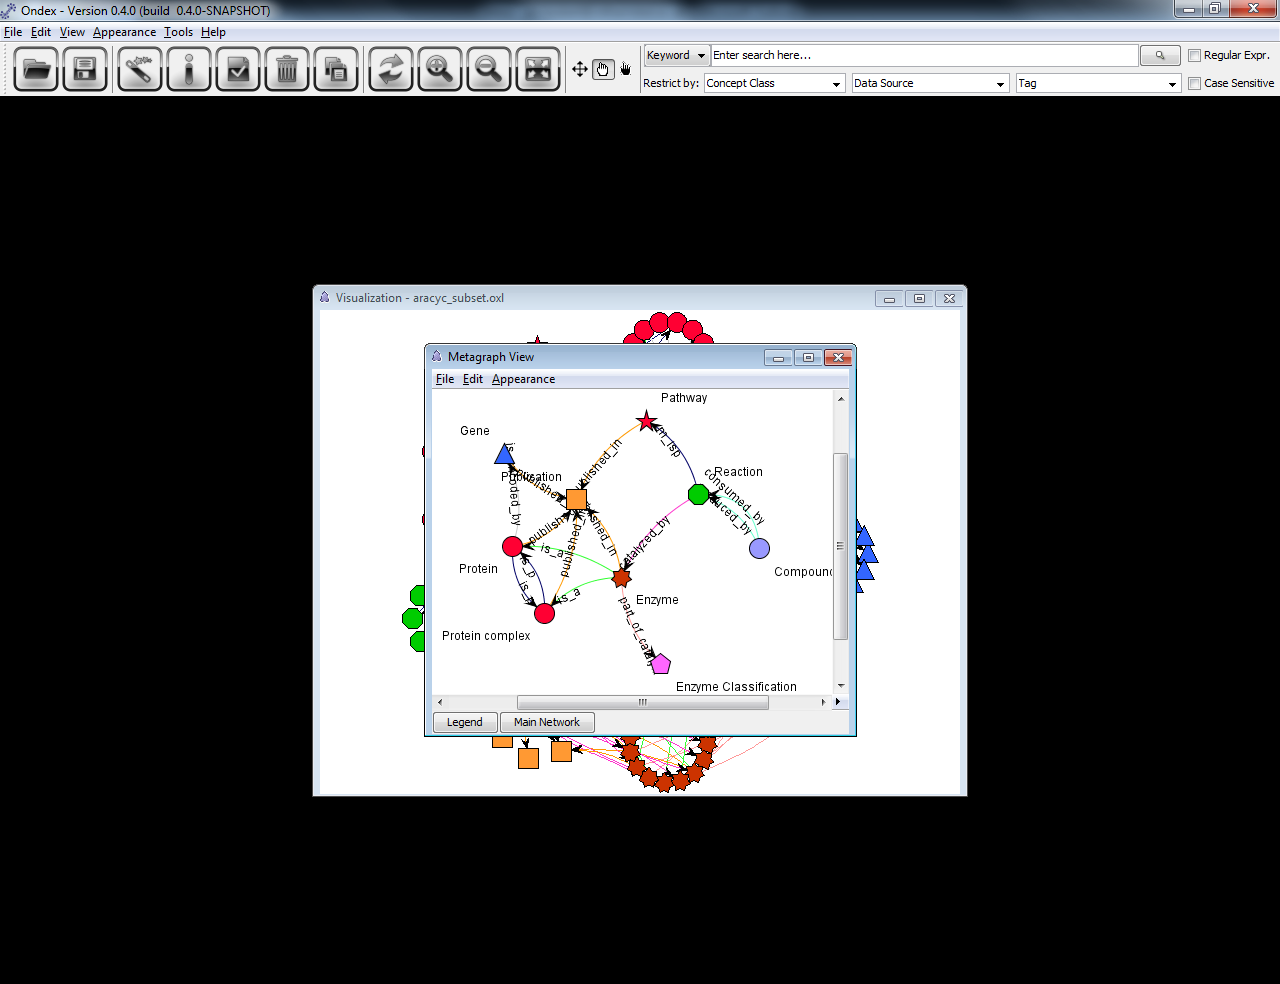
\includegraphics[scale=0.3]{images/Jun12/launched_aracyc_subset.png}
\caption{Metagraph - AraCyc}
\label{fig:metagraph_aracyc}
\end{figure}

The first window that shows is the ``Metagraph View''. Below this window is the main visualisation window for the network.
\emph{Note:} the main network will be minimized in the bottom left-hand side corner if the whole graph contains more than 2000 concepts or relations (in which case it is a good idea to filter it first, see Section \ref{sec:analysing}), otherwise it will appear behind the metagraph (as it is here). 

The metagraph gives an overview of all the different types of concepts present on the main network, as well as all the different types of relations which connect them.

The metagraph view has 2 buttons at the bottom of its window (for more information, Section \ref{sec:ref_metagraph} explains its menu):
\begin{itemize}
\item Legend: will pop up a window which displays a modifiable colour/shape legend as well as 
the number of concepts and relations in the network for concept classes, data sources, relation types and evidence types
\item Main Network: will open the main network visualisation window if it was minimized or just set focus to it
\end{itemize}


\exerciserule
\textbf{Exercise}
Trying to understand the metagraph before opening the main network usually helps. 
The main network is loaded with the ``Circular'' layout applied initially, which is an arrangements of all the concept classes (one small circle each) in the network on a big circle.

Rearranging concepts in the metagraph should give you a better understanding of its content. 
Figure \ref{fig:metagraph_rearranged} is an example of how the metagraph can be laid out.
\begin{figure}[H]
\centering
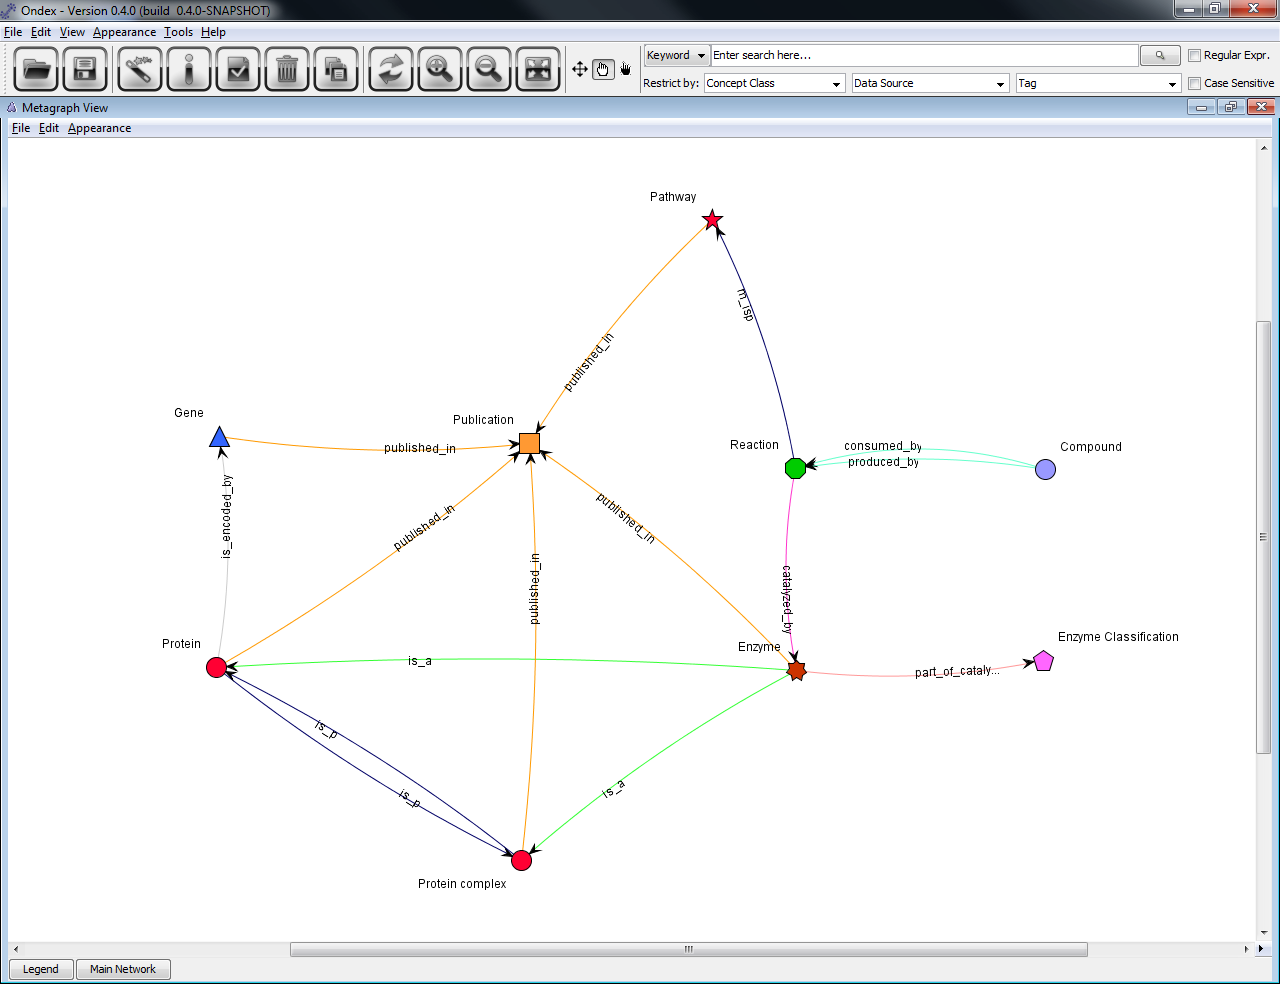
\includegraphics[scale=0.3]{images/Jun12/aracyc_rearranged_metagraph.png} 
\caption{Rearranged metagraph of AraCyc}
\label{fig:metagraph_rearranged}
\end{figure}
A protein is encoded by a gene (is\_encoded\_by).
A protein is part of a protein complex (is\_p).
An enzyme is a protein or a protein complex (is\_a).
An enzyme has a catalysing class EC (part\_of\_cataly...).
A compound is consumed by or produced by a reaction (consumed\_by, produced\_by).
A reaction is a member, is part of a pathway (m\_isp).
A reaction is catalysed by an enzyme (catalyzed\_by).
Finally, most concepts can be mentioned in publications (published\_in).

\exerciserule
\textbf{Exercise}
Right-click on nodes or edges in the metagraph displays the number of entities of that type in the network. 
It also gives users the opportunity to deselect ``Visible''. This will make concepts/relations of that type invisible in the main network. 
Nodes or edges in the metagraph for which all concepts/relations are invisible in the main network will appear in a paler colour.

\emph{Note:} Making concepts/relations invisible in the network will not delete them from the network altogether. 
If you wish to do so, use menu Edit -$>$ Delete Hidden Items. A window will pop up asking you for confirmation.

\exerciserule
\textbf{Exercise}
In the legend, clicking on colours/shapes will allow you to pick different colours/shapes for concept classes, 
data sources, relation types and evidence types (see 4 tabs in the legend window). 

For example, the concept class protein is of the same colour as the concept class pathway.
In order to make it more distinct, we can change its colour by clicking on the coloured rectangle (first column).
Figure \ref{fig:aracyc_click_colour} is obtained.
\begin{figure}[H]
\centering
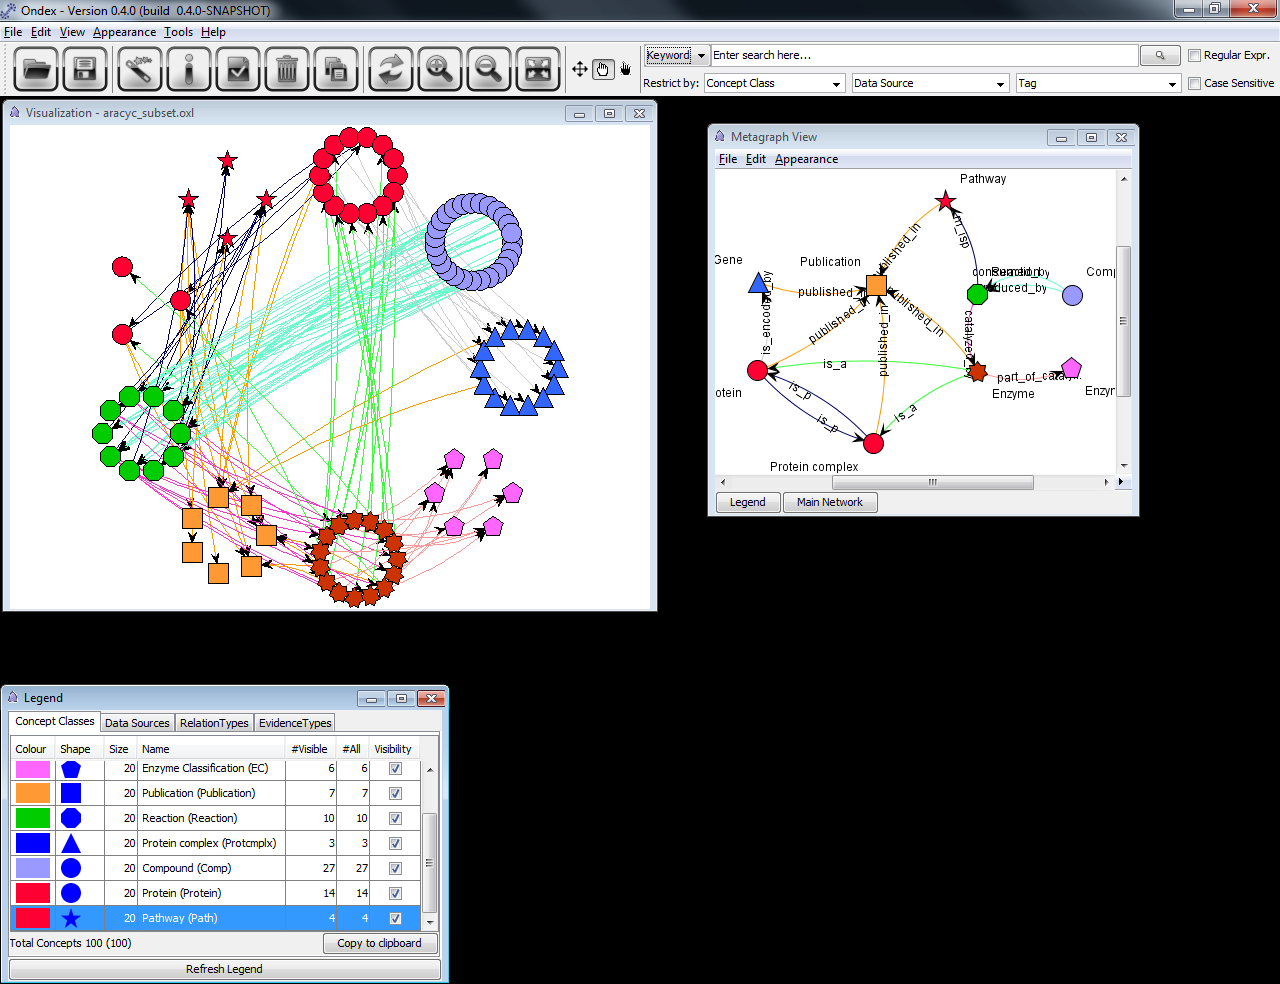
\includegraphics[scale=0.3]{images/Jun12/aracyc_colour_CC_from_legend.png} 
\caption{Click on a colour in the legend. A window pops open to change colours}
\label{fig:aracyc_click_colour}
\end{figure}

Clicking on the coloured rectangle pops open a ``Pick a colour'' window (see Figure \ref{fig:aracyc_pick}).
\begin{figure}[H]
\centering
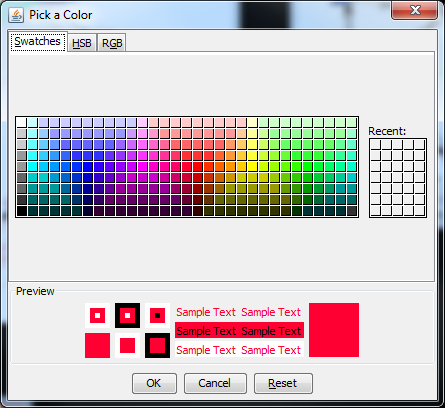
\includegraphics[scale=0.5]{images/Jun12/aracyc_pick_a_colour.png} 
\caption{Select a colour of your choice}
\label{fig:aracyc_pick}
\end{figure}

Select a colour, click on OK to obtain Figure \ref{fig:aracyc_changed_colour}.
\begin{figure}[H]
\centering
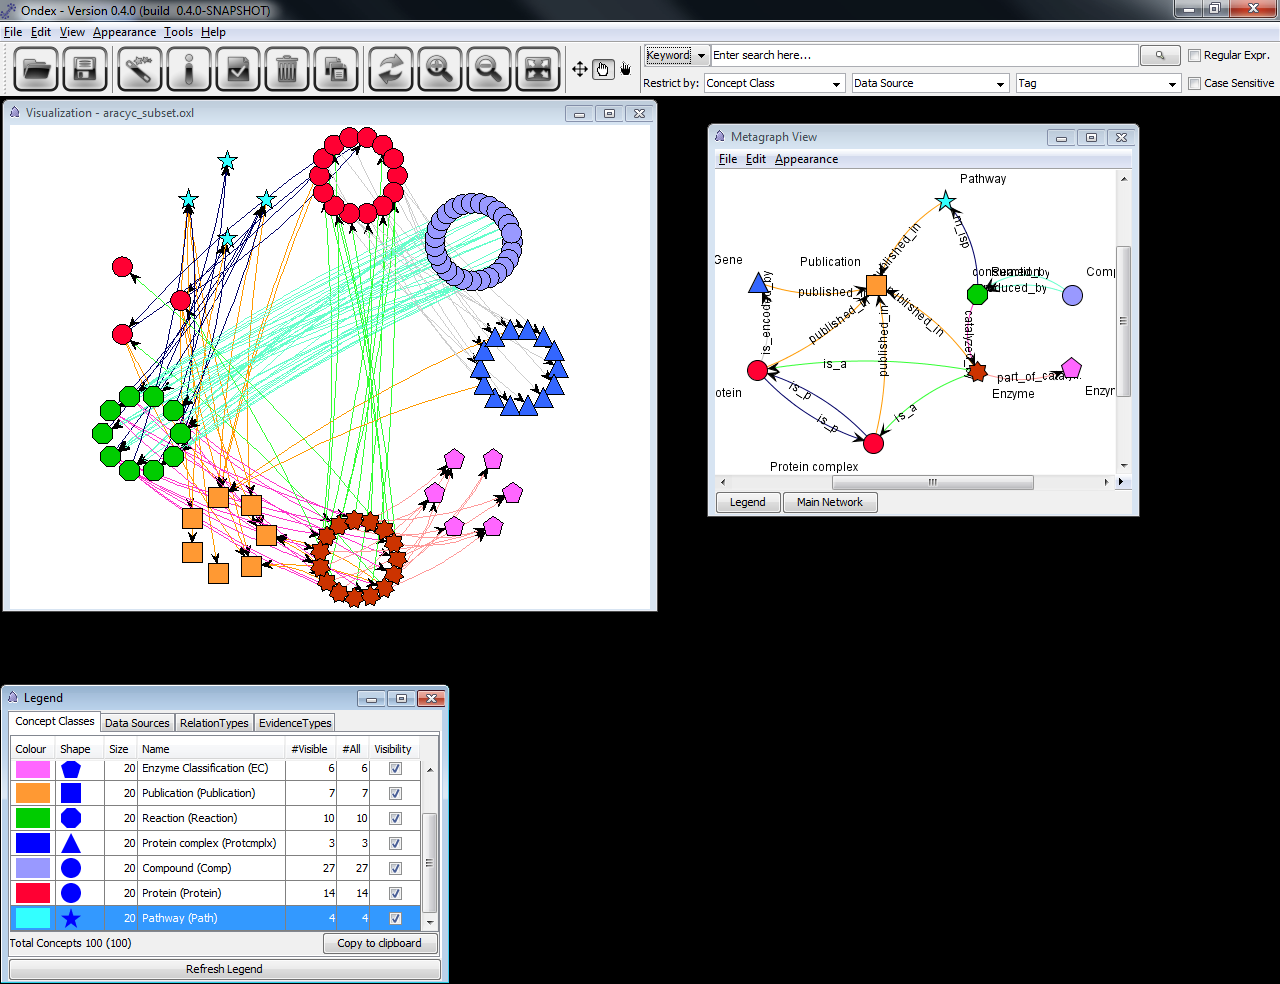
\includegraphics[scale=0.3]{images/Jun12/aracyc_colour_changed_from_legend.png} 
\caption{The colour of the concept class pathway has changed to turquoise}
\label{fig:aracyc_changed_colour}
\end{figure}

\exerciserule

The legend has four tabs: Concept Classes, Data Sources, Relation Types and Evidence Types. 
Figure \ref{fig:aracyc_legend_other_tabs} shows the Relation Types tab for this example.
Each tab displays the number of visible concepts/relations as well as the total number ({\it{i.e.}} including invisible items) in separate columns.
This window also allows you to select/deselect the check-boxes to make certain items visible/invisible in the visualisation window.
Furthermore, at the bottom of the legend window a total number is shown and a ``Copy to clipboard" button which enables users to copy/paste these numbers into other applications to keep track of them if needed.
\begin{figure}[H]
\centering
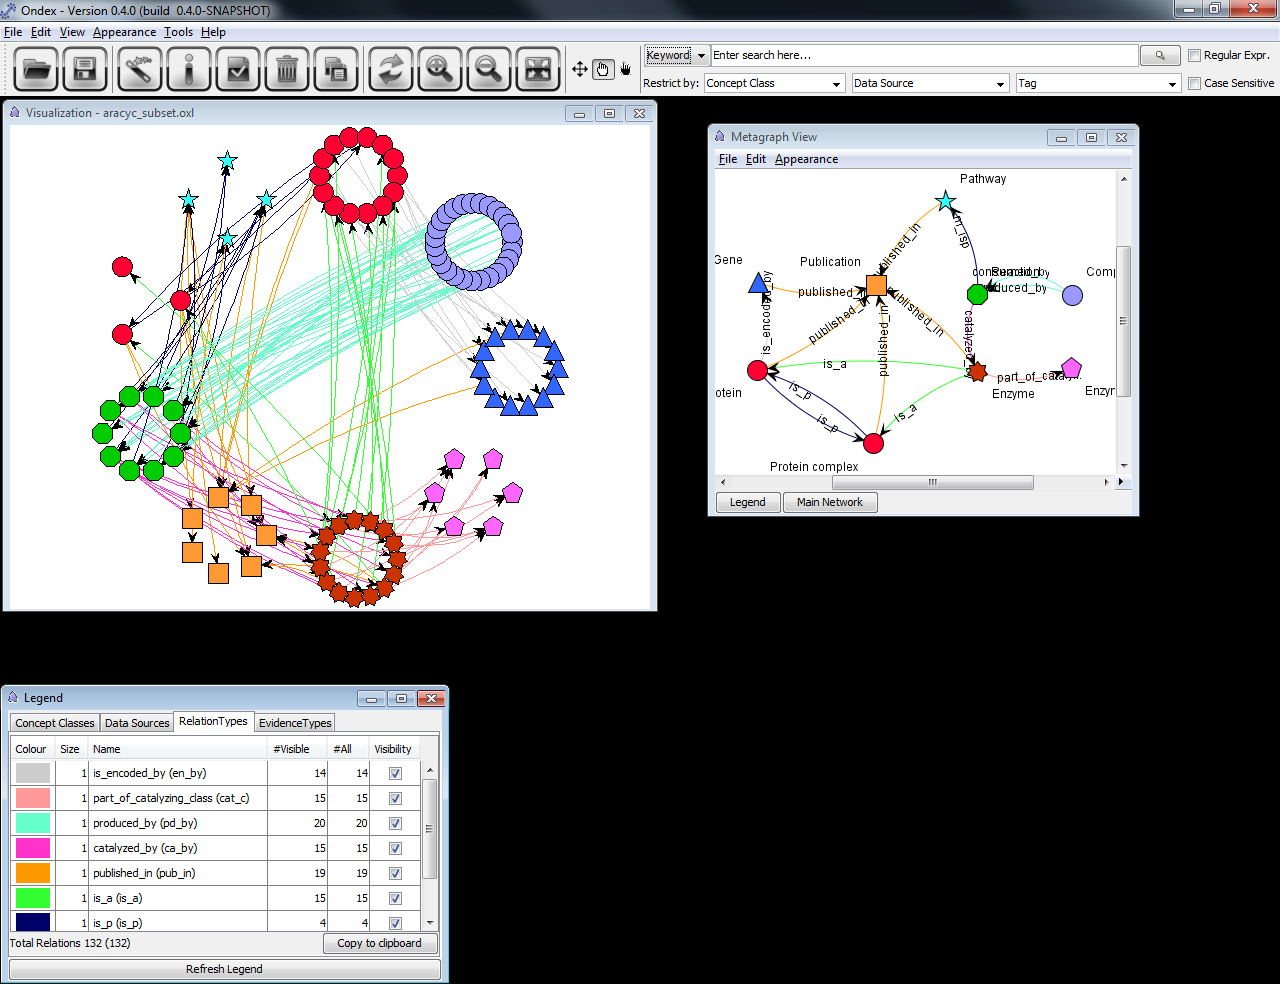
\includegraphics[scale=0.3]{images/Jun12/aracyc_legend_other_tabs.png} 
\caption{The Relation Types tab in the legend}
\label{fig:aracyc_legend_other_tabs}
\end{figure}

\emph{Advanced tip:} The experimental export plug-in "Graph Information Export" can be used when more thorough reports of the data are required for data integration purposes and can save a lot of time compared to manual inspection of graphs as it offers lists of accessions along with examples and percentages.
Such reports are particularly useful for setting the parameters of the accession based mapping method 
(see Sections \ref{sec:accmapping_examples} and \ref{sec:accmapping}) correctly.


%%%%%%%%%%%%%%%%%%%%%%%%%%%%%%%%%%%%%%%%%%%%%%%%%%%%%%%%%%%%%%%%%%%%%%%%%%%%%%%%%%%%%%%%%%%%%%%%%%%%%%%%%%%%%%%%%%%%%%%%%%%%%%%%%%%%%%%%%%%%%%%%%%%%%%%%%%
\section{Analysing Networks}
\label{sec:analysing}
If the main network is large and wasn't opened behind the metagraph, you can click on ``Main Network'' in the ``Metagraph View'' window or maximize the visualisation window that has been sitting in the bottom left-hand side corner all along.
Opening the visualisation window can take some time when there are a lot of concepts and relations to draw.
Two options are possible at this stage:
\begin{enumerate}
\item If your computer is fast or you are patient, you can open the main network as described above
\item Otherwise you can use filters (under Tools menu) or a search (search bar, top-right corner) to extract a smaller sub-network.
If the data contains ``tags'' (predefined subsets of the data) then using the Tag Filter is another possibility.
\end{enumerate}

%%%%%%%%%%%%%%%%%%%%%%%%%%%%%%%%%%%%%%%%%%%%%%%%%%%%%%%%%%%%%%%%%%%%%%%%%%%%%
\subsection{Filtering}
\label{sec:filtering}

For example here, rather than looking at the whole subset of AraCyc in Figure \ref{fig:complete_subset_aracyc}, 
let us select a single pathway to display.

\begin{figure}[H]
\centering
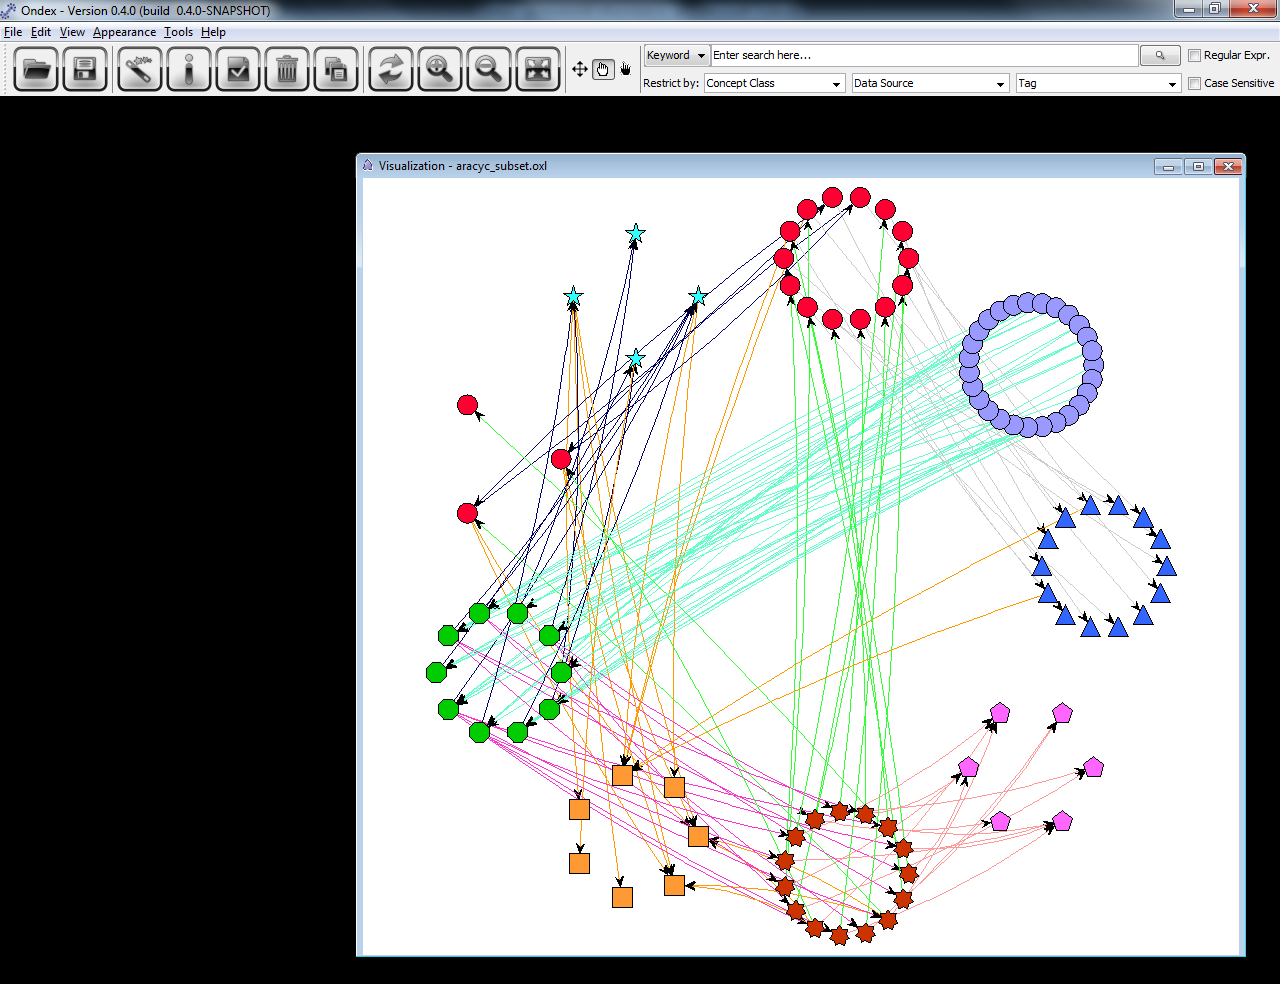
\includegraphics[scale=0.3]{images/Jun12/aracyc_circular_subset.png} 
\caption{Subset of AraCyc drawn with the circular (default) layout}
\label{fig:complete_subset_aracyc}
\end{figure}

In order to do so, select the Tag Filter under menu Tools -$>$ Filters.
This filter is fully explained in the ``F1 help'' documentation of Ondex.
It offers the possibility of combining different tags.
For now, we will simply filter down the network to a single pathway.
Let us select GDP-L-fucose biosynthesis II as shown in Figure \ref{fig:aracyc_pick_tag}
(click on the view tag cell and select GDP-L-fucose biosynthe... from the list of possible tags).

\begin{figure}[H]
\centering
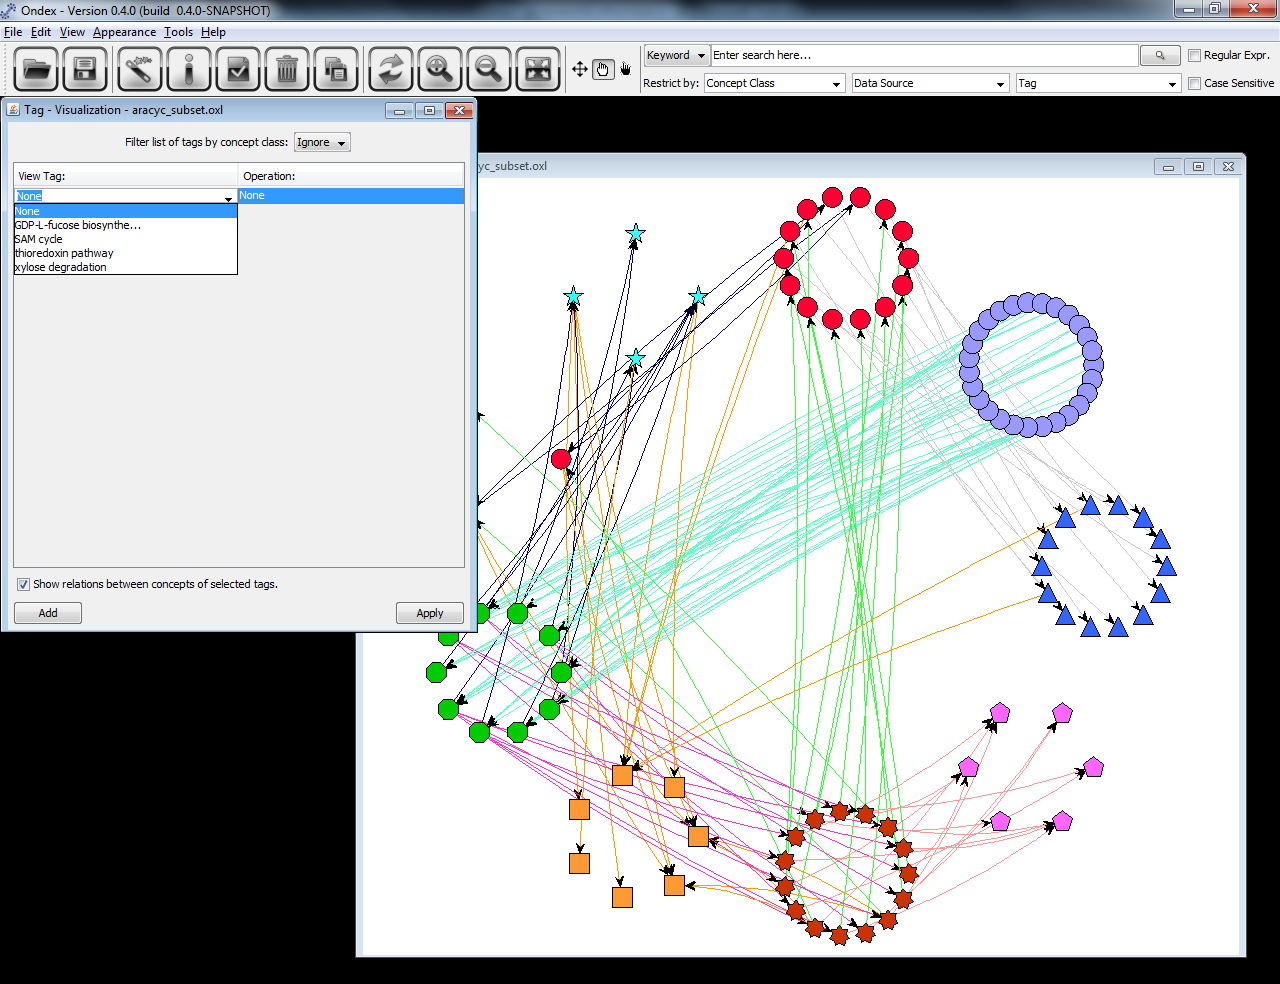
\includegraphics[scale=0.3]{images/Jun12/aracyc_pick_tag.png} 
\caption{Pick a tag from the drop-down list}
\label{fig:aracyc_pick_tag}
\end{figure}

Figure \ref{fig:aracyc_gdp_fucose_II} shows the resulting network.
\begin{figure}[H]
\centering
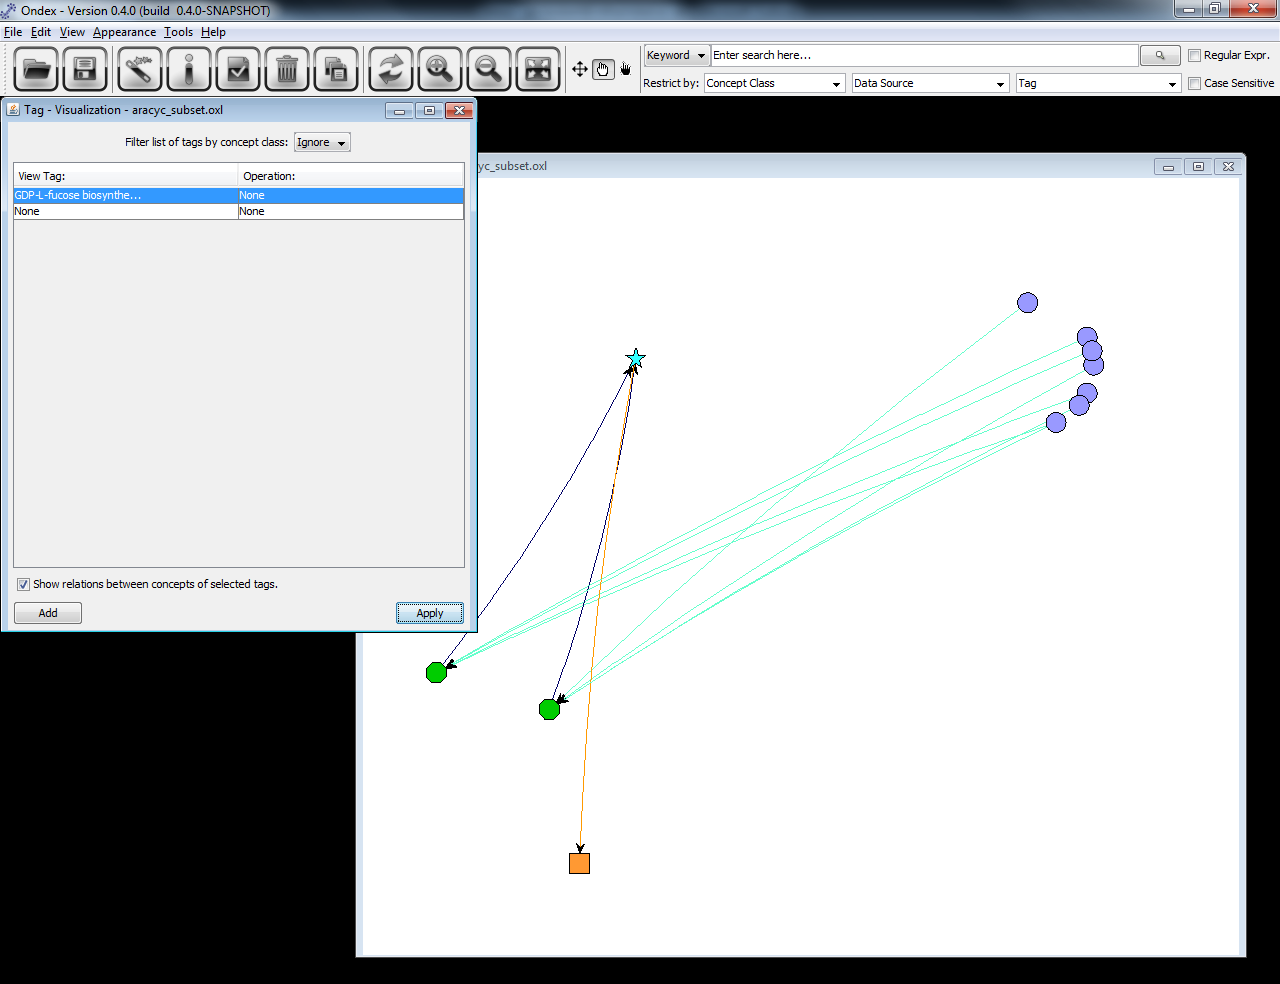
\includegraphics[scale=0.3]{images/Jun12/aracyc_gdp_fucose_II.png} 
\caption{The GDP-L-fucose biosynthesis II pathway from the AraCyc database}
\label{fig:aracyc_gdp_fucose_II}
\end{figure}

We can use Appearance -$>$ Layouts -$>$ More -$>$ Hierarchical for Ondex to organise the concepts hierarchically (see Figure \ref{fig:aracyc_gdp_fucose_hierarchical}).
\begin{figure}[H]
\centering
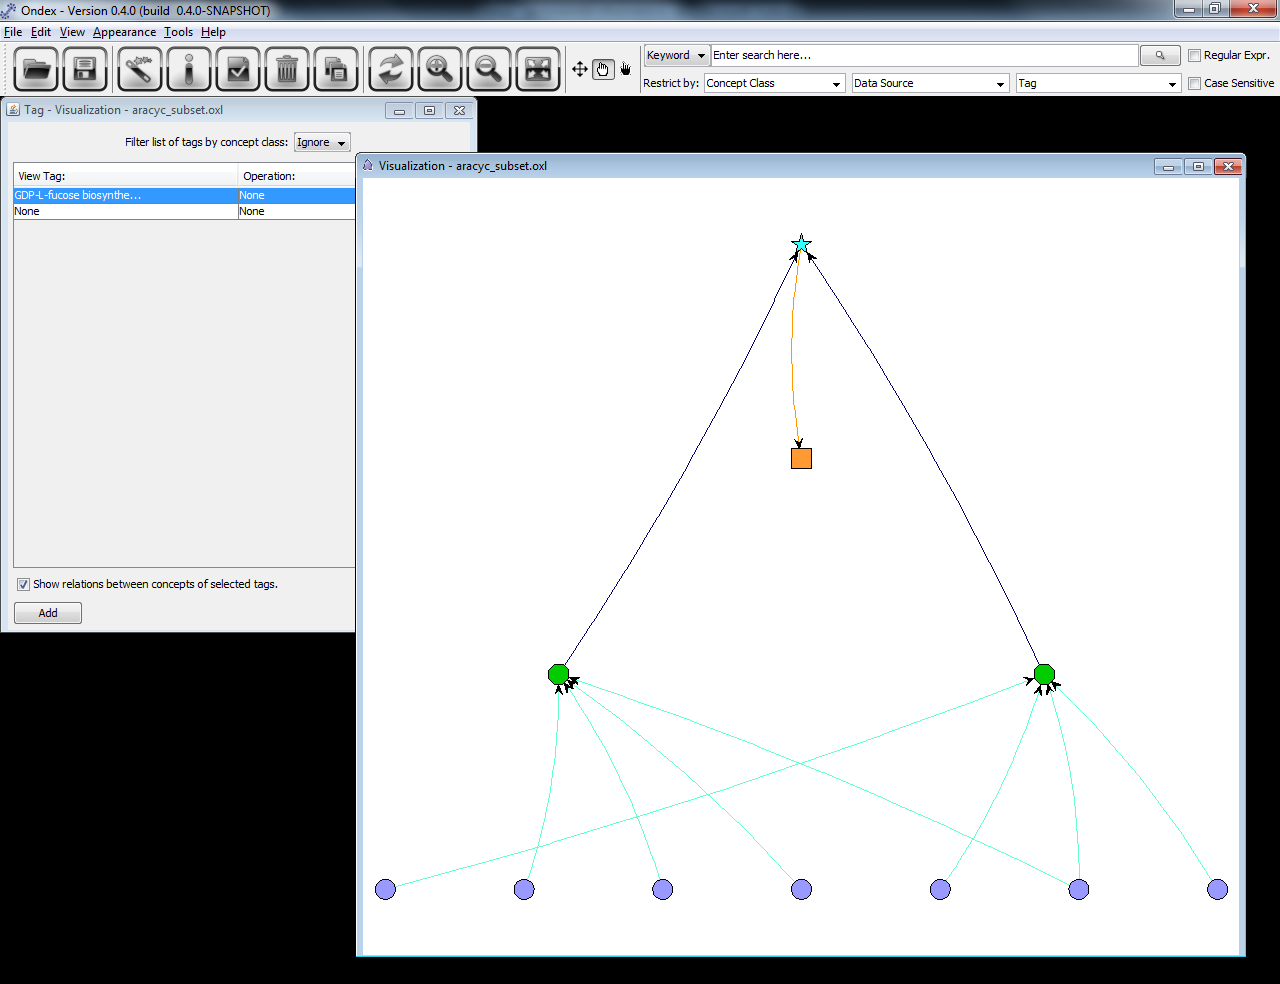
\includegraphics[scale=0.3]{images/Jun12/aracyc_gdp_fucose_hierarchical.png} 
\caption{Hierarchical layout of the GDP-L-fucose biosynthesis II pathway from the AraCyc database}
\label{fig:aracyc_gdp_fucose_hierarchical}
\end{figure}

You can then select a concept, for example, the pathway itself (click on it, it will become yellow).
Then you can click on the ``i'' icon (a tool-tip shows when you mouse over the icon) to see information about the selected pathway, as shown in Figure \ref{fig:aracyc_gdp_fucose_iteminfo}. \emph{Note:} You can ignore the ``Taxonomy lookup'' by clicking on the given option ``No, don't ask again''.


The item information gives a link to the AraCyc website at the very bottom of the window under section ``Accessions''.
Clicking on this link opens a web browser as shown in \ref{fig:aracyc_info_website}.
\begin{figure}[H]
\centering
\subfigure[Item Information icon launches an information window]{
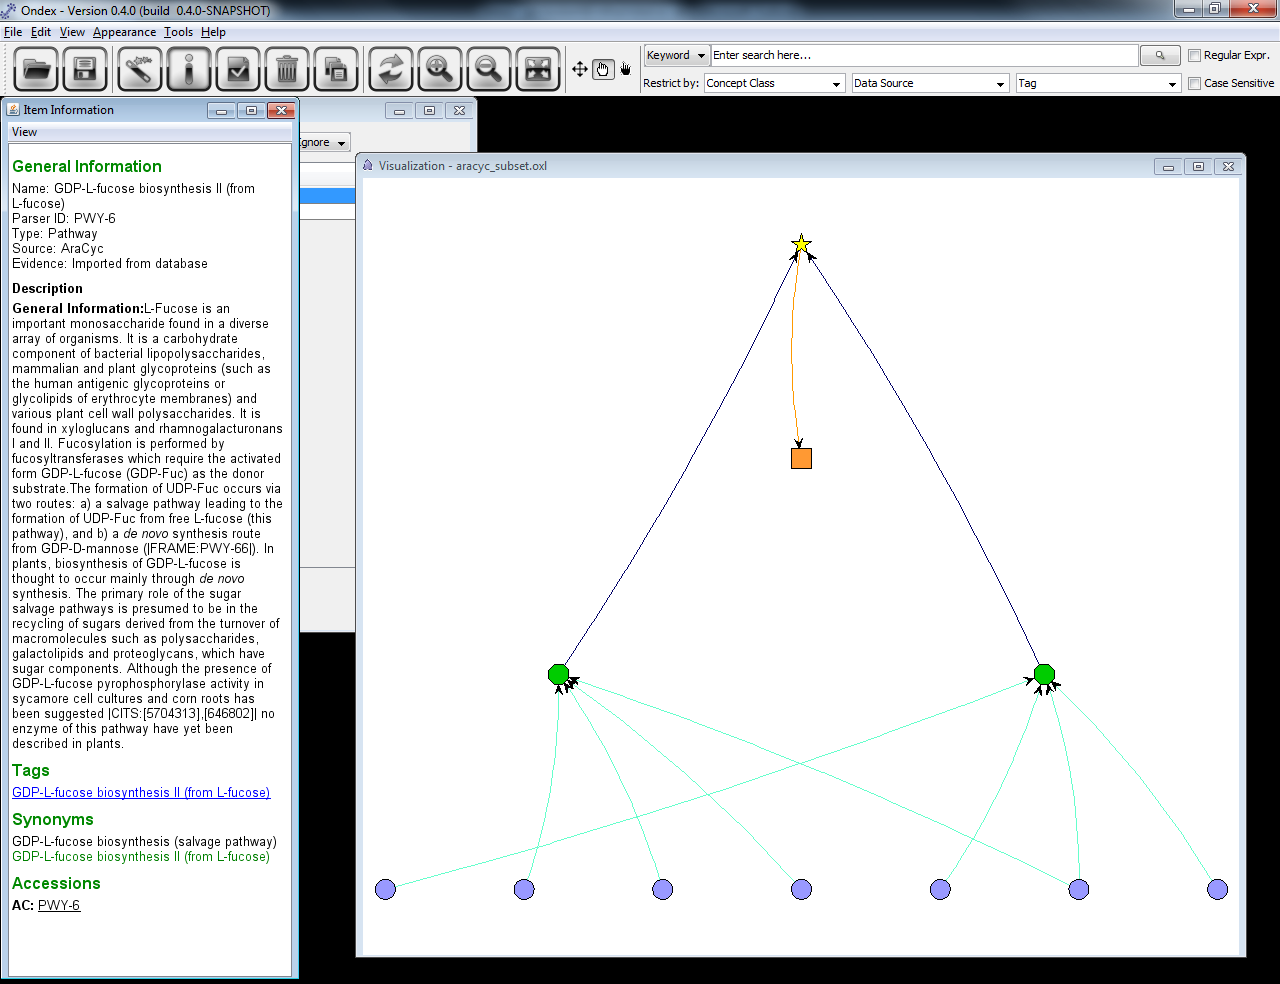
\includegraphics[scale=0.3]{images/Jun12/aracyc_gdp_fucose_iteminfo.png} 
\label{fig:aracyc_gdp_fucose_iteminfo}
}
\subfigure[The Aracyc website showing the selected pathway]{
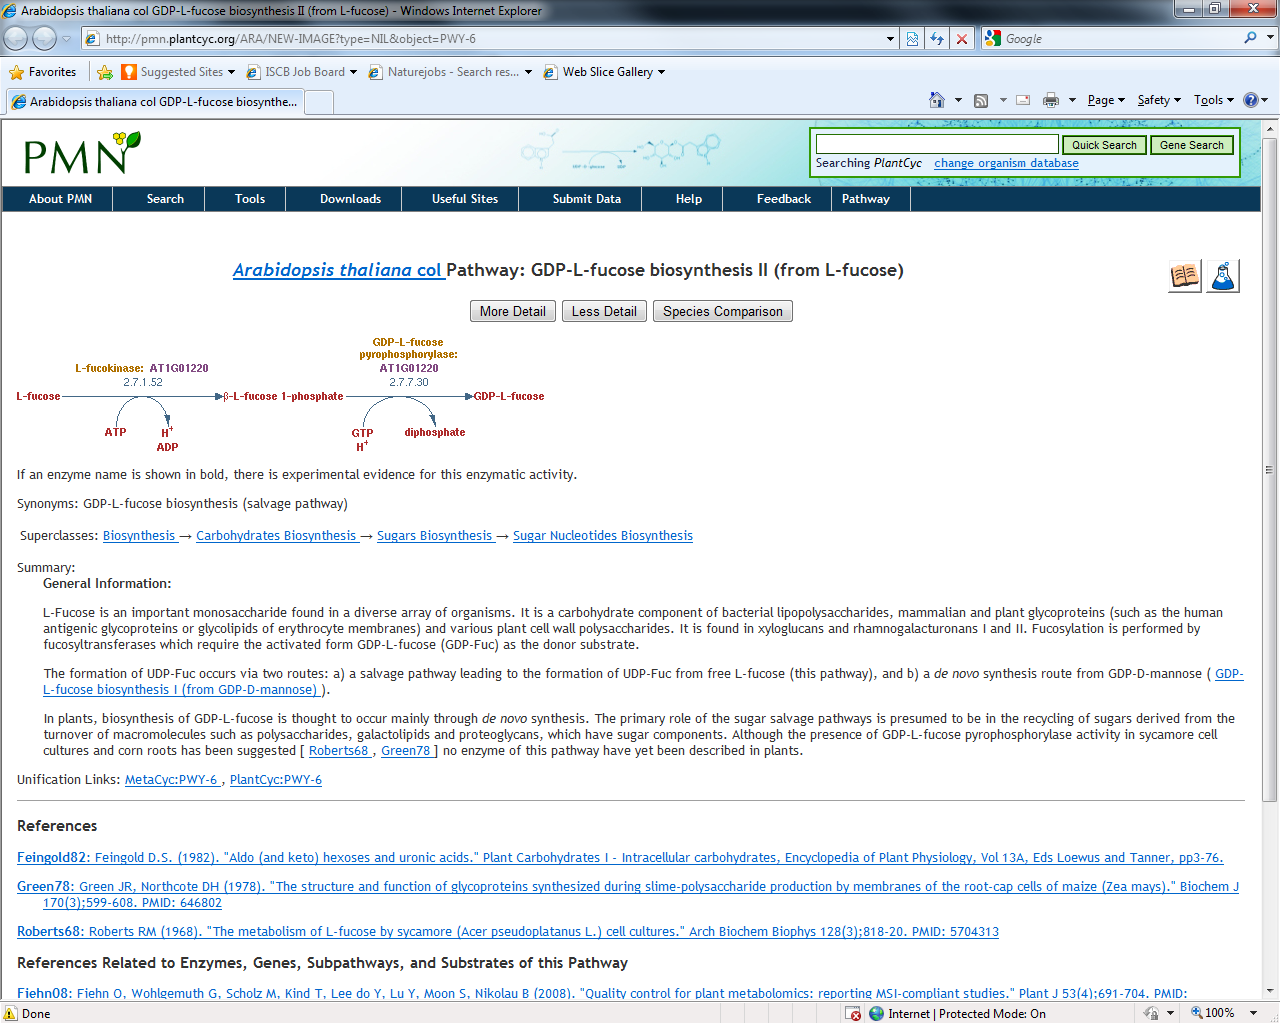
\includegraphics[scale=0.3]{images/Jun12/aracyc_gdp_fucose_webpage.png} 
\label{fig:aracyc_gdp_fucose_webpage}
}
\label{fig:aracyc_info_website}
\caption[optional]{Item information and its links to websites}
\end{figure}

\vspace{0.5cm}
\exerciserule
\textbf{Exercise }
Study the reaction shown on the website and try to understand how it is represented in Ondex.

\emph{Help:} The first thing you might want to do is use the menu Appearance -$>$ Labels to add concept and relation labels 
on the network so you know what is what without needing the ``Item Information'' window. Use
Appearance -$>$ Labels -$>$ Both to show labels of concepts and relations.

\emph{Help:} To move concepts around, you can either pick them (in picking mode - ``white hand'' icon before search bar in the tool-bar or menu Edit -$>$ Mouse mode -$>$ Picking) and move them one by one.
You may also press shift to select a few concepts with the left mouse button and
using the left mouse button again you can drag these group of concepts around.

Figure \ref{fig:aracyc_gdp_fucose_sorted} shows what can be obtained by following this process. 
\emph{Note:} the ``Metagraph View'' window is not shown on this screenshot.
The reactions previously shown on the website have been reconstituted. 
Here, the compound that is a product of the first reaction and a substrate of the second has been selected and is automatically shown in the ``Item Information'' window.\\ 
\emph{Note:} SMILES stand for ``simplified molecular input line entry specification''.\\
\emph{Note:} If you have closed the Legend (previously launched from the metagraph view window), you may launch it again using View -$>$ Legend to check how many compounds are currently displayed.
\begin{figure}[H]
\centering
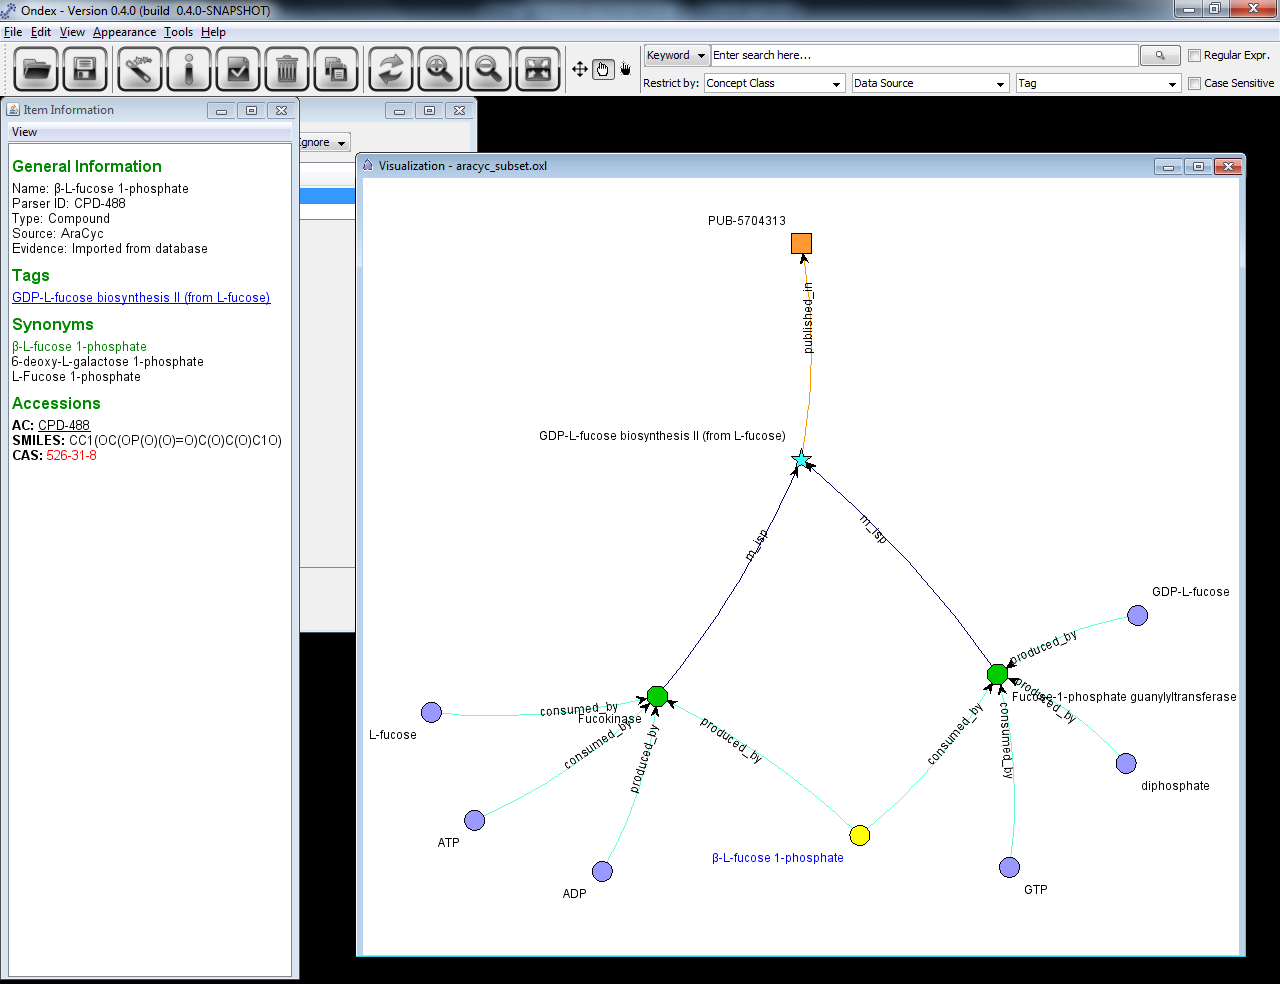
\includegraphics[scale=0.3]{images/Jun12/aracyc_gdp_fucose_sorted.png} 
\caption{The GDP-L-fucose biosynthesis II pathway as shown in Figure \ref{fig:aracyc_gdp_fucose_webpage} layout in Ondex}
\label{fig:aracyc_gdp_fucose_sorted}
\end{figure}
\exerciserule

Other filters and annotators (as well as layouts) are available and documented in Ondex.
Users can press F1 to access this documentation at any time.
They can also place their mouse over tool-tips for a short description to pop up,
or click on the blue question mark icon for the documentation window to open.
In Tutorial\_files/Annotators\_and\_Filters/readme\_annotators\_filters.txt explains which file (within that directory) 
is used for each example in the documentation's screenshots (to allow users to play with the data themselves).

%%%%%%%%%%%%%%%%%%%%%%%%%%%%%%%%%%%%%%%%%%%%%%%%%%%%%%%%%%%%%%%%%%%%%%%%%%%%%
\subsection{Searching}
\label{sec:search}
Ondex includes a Search feature (see Figure \ref{fig:vis_search_bar}), which enables you to quickly find concepts in the network containing a given keyword or by chemical similarity to a given SMILES or InChI qualifier.
\begin{figure}[H]
\centering
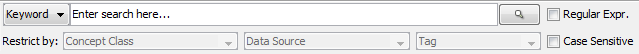
\includegraphics[scale=0.6]{images/Jun12/search_bar.png} 
\caption{The Ondex search bar}
\label{fig:vis_search_bar}
\end{figure}

For example, searching for keyword fucose in our current graph will give use the results shown in Figure \ref{fig:search_results}
\begin{figure}[H]
\centering
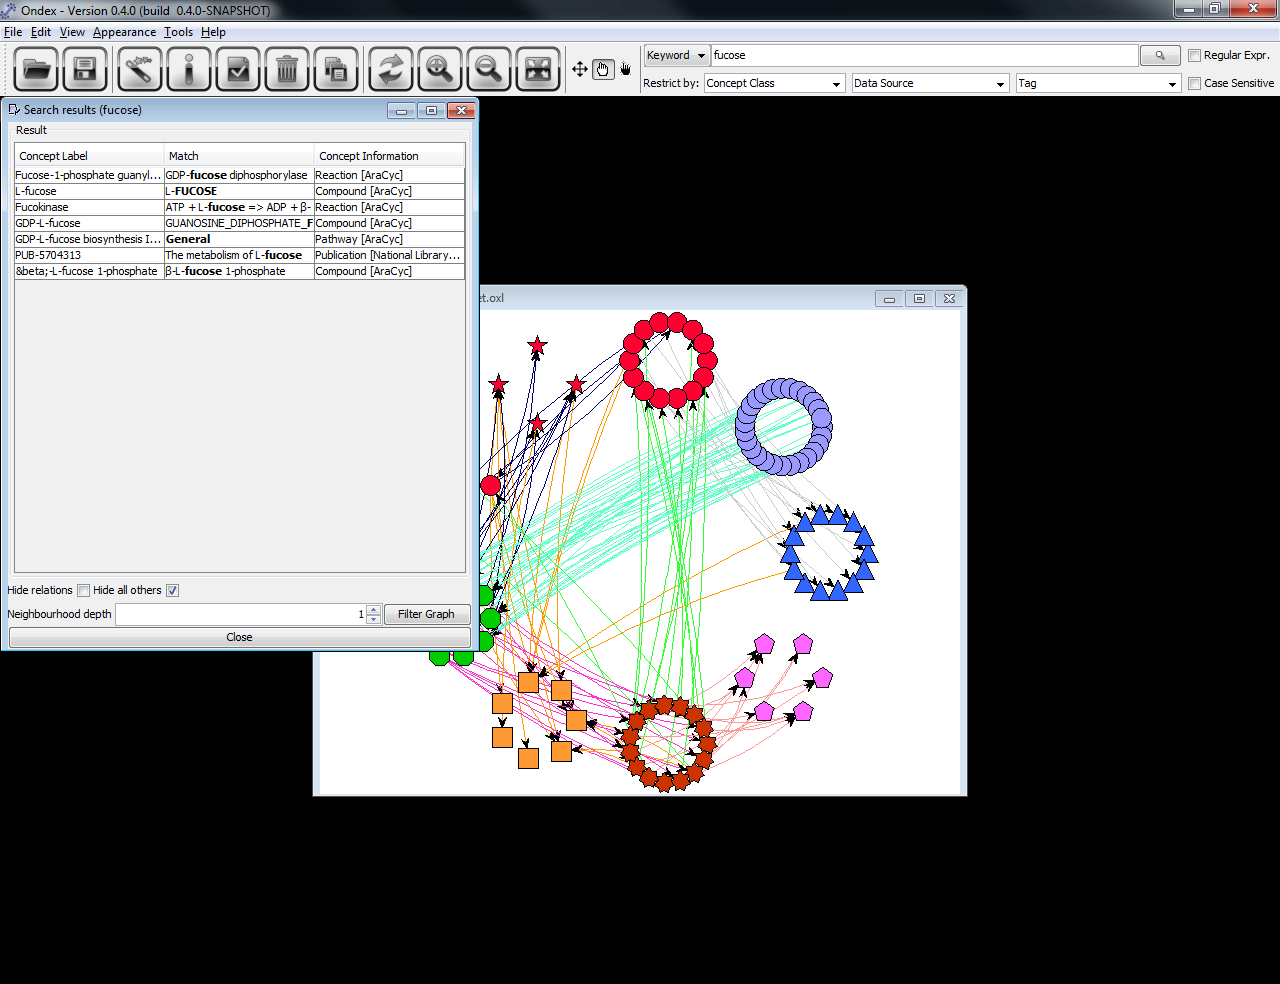
\includegraphics[scale=0.3]{images/Jun12/aracyc_search_fucose.png} 
\caption{Search results for ``fucose'' in Aracyc}
\label{fig:search_results}
\end{figure}

If you select (single click) one item in the search results, you will need to single click on the icon ``Zoom In'' in order for Ondex to zoom in and center on this particular concept. 
You can then use the mouse scroll wheel to zoom even closer to the concept.
If you select several items (using the Control key) in the search results, Ondex will automatically zoom in to show all those items as close as possible.

\vspace{0.5cm}\textbf{Configuring an Ondex Search }
\begin{itemize}
\item At the end of the tool-bar, there are 2 options that can be configured for keyword based search. 
If you select ``Regular Expression'', you may enter a Java regular expression. An example would be: AT$\backslash$dG.
It will match ``AT'' followed by any digit and ``G''. For more information on regular expressions in Java, please visit \url{http://docs.oracle.com/javase/tutorial/essential/regex/}.
If you select ``Case Sensitive'', the search will be sensitive to lower/upper case of each character.
\item Under the search box, there are 3 drop-down lists which allow users to restrict their search (by Concept Class, Data Source or Tag).
An example is provided in the next section's exercise.
\end{itemize}

%%%%%%%%%%%%%%%%%%%%%%%%%%%%%%%%%%%%%%%%%%%%%%%%%%%%%%%%%%%%%%%%%%%%%%%%%%%%%
\subsection{Right-clicking}
\label{sec:right-clicking}
Right-clicking on one or a selection of concepts/relations also offers users the possibility to narrow down the graph to what they are interested in.
Close all the windows you have opened in Ondex (View -$>$ Windows -$>$ Close All).

\begin{itemize}
\item Go to File -$>$ Open  (or click on the first button in the icon bar)
\item You should see an Open File Dialog
\item Open the Tutorial\_files/Main\_part folder, select poplar\_exercise1.oxl and click on open
\end{itemize}

This graph results from a data integration (see Chapter \ref{cha:integration}) pipeline using information from JGI,
UniProtKB, TAIR, Gramene, Gene Ontology (GO), GOA (GO Annotations), TraitOnt, PlantOnt, Medline, AraCyc, PoplarCyc and Pfam
which aims to identify genes controlling biomass production in willow.
The willow genome is not yet sequenced. Poplar is the first tree with fully sequenced genome but
not much is known yet about the function of poplar genes.
This study (see Chapter \ref{cha:qtl}) uses a comparative genomics approach to compare poplar to {\it{Arabidopsis}} and rice.

The metagraph shows a lot of different concept classes and relation types,
including ``Molecular Function'', ``Biological Process'' and ``Cellular Compartment'' - the 3 GO categories (see Figure \ref{fig:vis_poplar_metagraph}).
\begin{figure}[H]
\centering
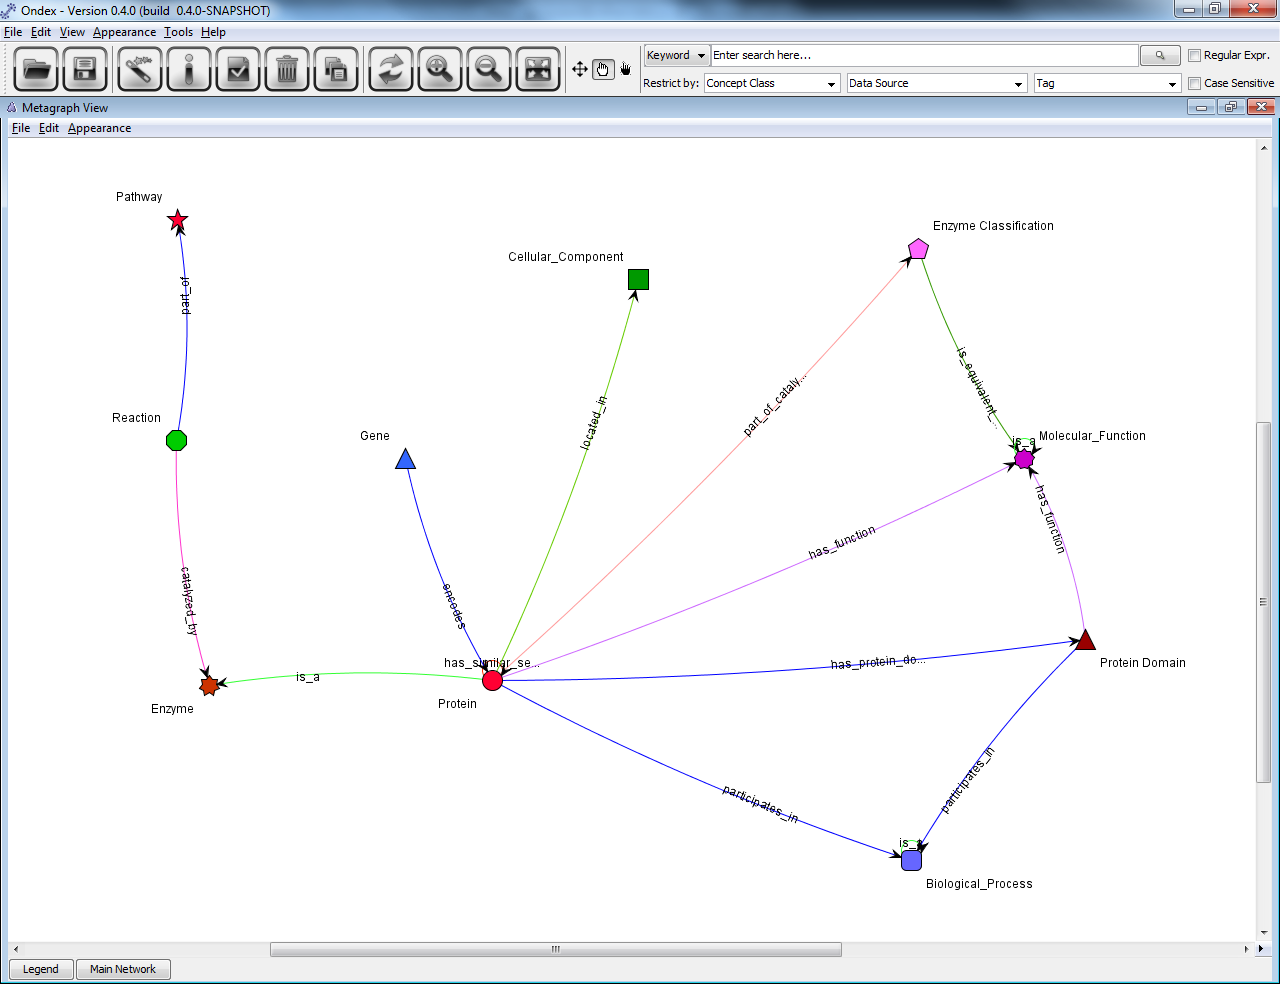
\includegraphics[scale=0.3]{images/Jun12/poplar_ex1_metagraph.png} 
\caption{Metagraph - poplar\_exercise1.oxl}
\label{fig:vis_poplar_metagraph}
\end{figure}

\exerciserule
\textbf{Exercise}
In this exercise, we will look at a particular poplar gene (the only one in this subset). 
As it is lacking functional annotation, we wish to study the poplar protein it encodes, its homologous proteins 
and the GO terms they have been associated with. We will also investigate whether data integration has allowed linking this poplar protein to other kinds of information.
Use the search bar and a combination of right-clicks to get to Figure \ref{fig:poplar_result_exercise1} where only these concepts are visible on the graph.
\begin{figure}[H]
\centering
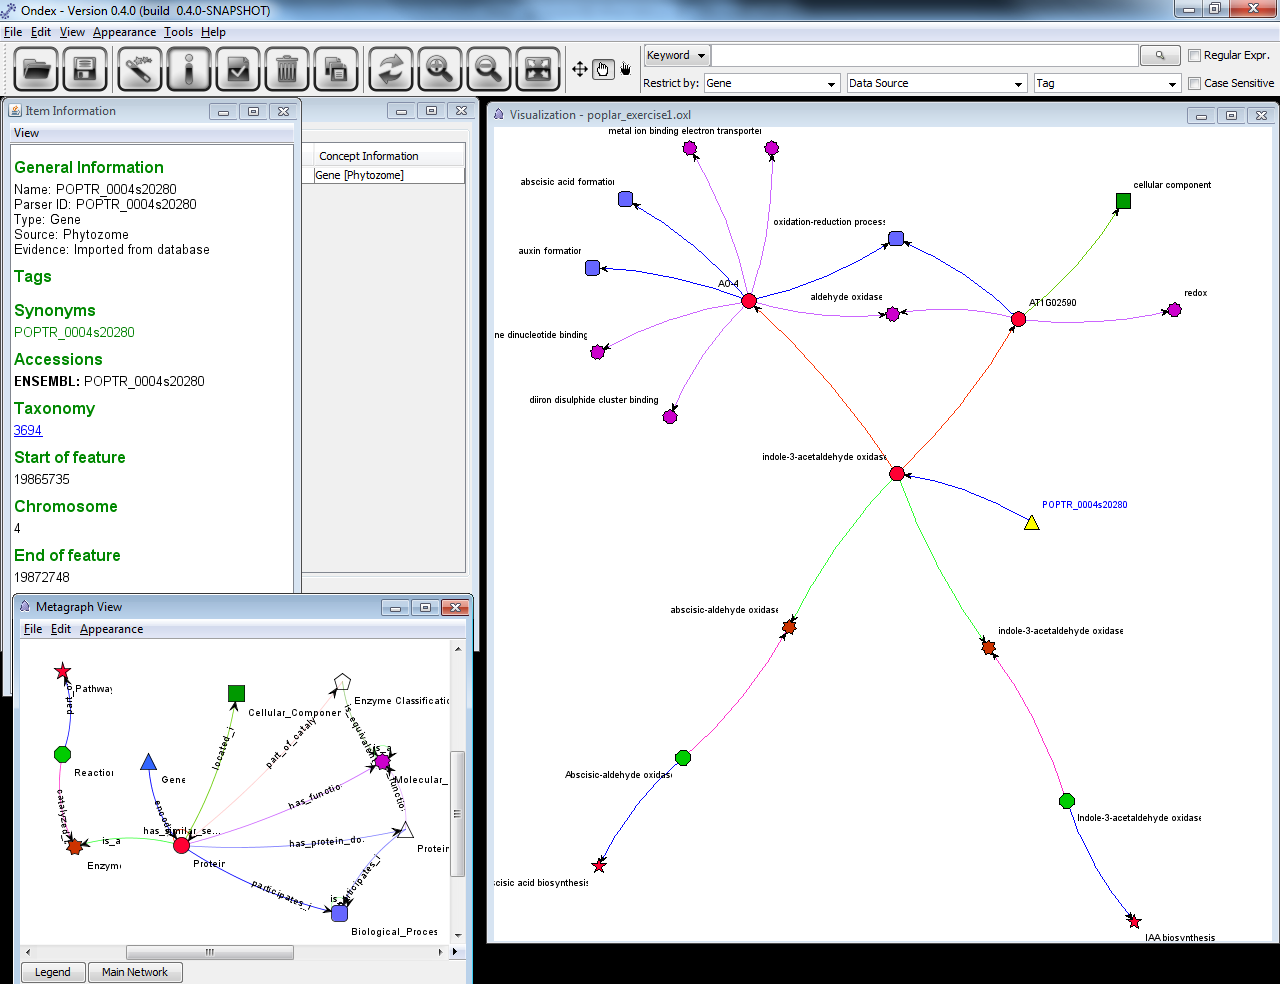
\includegraphics[scale=0.3]{images/Jun12/poplar_result_exercise1.png} 
\caption{Visualisation window (and part of metagraph) at the end of the exercise}
\label{fig:poplar_result_exercise1}
\end{figure}

\emph{Help:} 
\begin{itemize}
\item Clear the search bar, restrict the search to Concept Class Gene and hit enter. You should obtain only one result (because there was only one gene in this particular subset).
\item In the search results, select a neighbourhood depth of 1 and click on ``Filter Graph''.
\item Click on Main Network (from the metagraph or from the minimized window), you should see the gene you had searched for and the protein encoded by that gene.
\item Click on Appearance -$>$ Labels -$>$ Concepts to show concept labels.
\end{itemize}

We are now interested in looking at homologous proteins which might be annotated with GO terms.
\begin{itemize}
\item Right-click on the protein and select Show -$>$ Immediate Neighbours by Concept Class -$>$ Protein(2:2). (There are two of them and both are invisible at the moment.)
\item Select the homologous proteins and check their item information using the ``i'' icon or View -$>$ Item Info. You will find one is from rice and one {\it{Arabidopsis}}.
\item Select the two homologous proteins (click on one, it becomes yellow, press shift and select the second one)
\item Right-click and select Show -$>$ Immediate Neighbourhood and observe the 3 categories of GO terms one by one, see how many are shared by the two orthologous proteins.
\end{itemize}

Now let's investigate whether data integration has allowed linking our poplar protein to other kinds of information.
\begin{itemize}
\item From our poplar protein, select Show -$>$ Immediate Neighbourhood. Protein domains and two enzymes show.
\item From the enzymes, select Show -$>$ Immediate Neighbourhood. Two reactions get displayed.
\item From the reactions, select Show -$>$ Immediate Neighbours by Concept Class -$>$ Pathway (2:2). Two pathways show.
\item You may study the protein domains and decide to show their relations to visible concepts on the graph (right-click Show -$>$ Relations to other Visible Concepts).
To get to Figure \ref{fig:poplar_result_exercise1}, you will need to hide them. 
To do so, you may select one protein domain and select Hide -$>$ Same Concept Class.
\end{itemize}

%%%%%%%%%%%%%%%%%%%%%%%%%%%%%%%%%%%%%%%%%%%%%%%%%%%%%%%%%%%%%%%%%%%%%%%%%%%%%
\subsection{Annotating}
\label{sec:annotating}
Once a graph is filtered down to a region of interest, annotators (Tools -$>$ Annotators) allow you to scale your concepts/relations,
change their shapes and colours or display numerical data as charts based on the attributes they hold.
We will work on a data integration problem described in Section \ref{cha:qtl} and analyse the results using a few annotators. Other application cases also show case various annotators.

This example allows you to practice analysing networks in Ondex using a combination of the tools available.
Firstly, given a candidate gene (the only one in the graph) we wish to study its annotations and their GO hierarchy.
We also wish to annotate the molecular functions based on their information content.
To do so:
\begin{itemize}
\item Load the Tutorial\_files/Main\_part/poplar\_exercise1.oxl dataset
\item Select the only gene in the graph (or search for it as we did in the previous exercise).
\item Run the shortest path filter. The results are shown on Figure \ref{fig:poplar_result_shortestpath}. 
\begin{figure}[H]
\centering
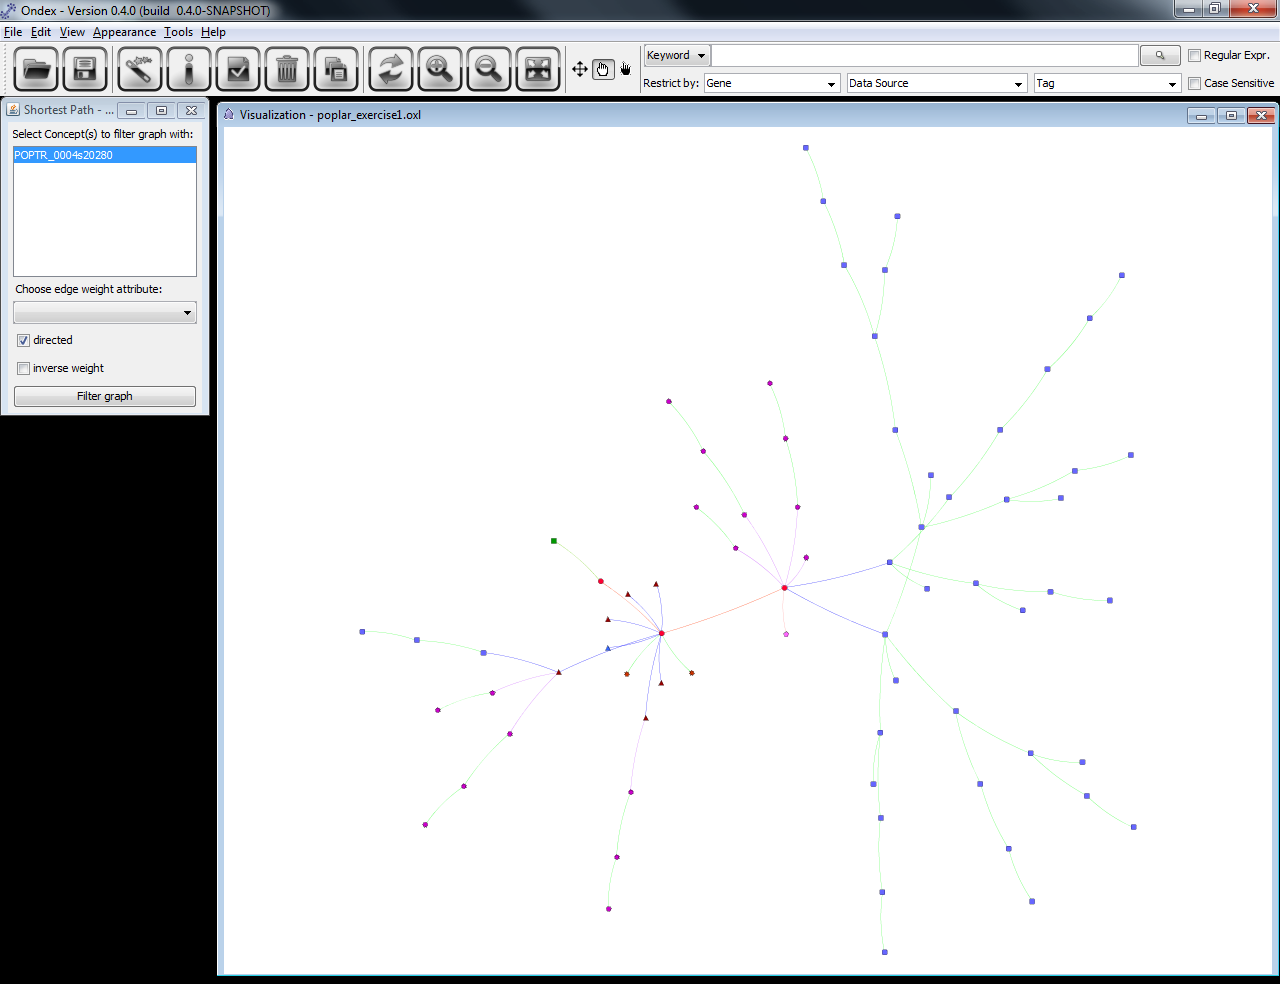
\includegraphics[scale=0.3]{images/Jun12/poplar_result_ex2_shortestpath.png} 
\caption{Screen-shot after applying the shortest path filter}
\label{fig:poplar_result_shortestpath}
\end{figure}

\emph{Help:}
	\begin{itemize}
	\item Tools -$>$ Filters -$>$ More -$>$ Shortest Paths -$>$ Shortest Path
	\item Select the gene (POPTR\_0004s20280)
	\item Do not select any edge weight attribute (from the drop-down list)
	\item Tick the box for directed (so that you can see the GO hierarchy)
	\item Click on ``Filter graph''
	\item Use the Gem layout (Appearance -$>$ Layouts -$>$ Gem)
	\item Use Appearance -$>$ Smooth Relations to make relations anti-aliased thereby smoother
	\end{itemize}

To analyse the information content within the GO hierarchy:
\item Run an annotator to scale the molecular functions concepts based on their attribute called ``Information Content''
(which is added to the data by running a Transformer (experimental) called ``Annotate Information Content'', see Section \ref{sec:integrator}). The results are shown on Figure \ref{fig:poplar_result_annIC}. 

\begin{figure}[H]
\centering
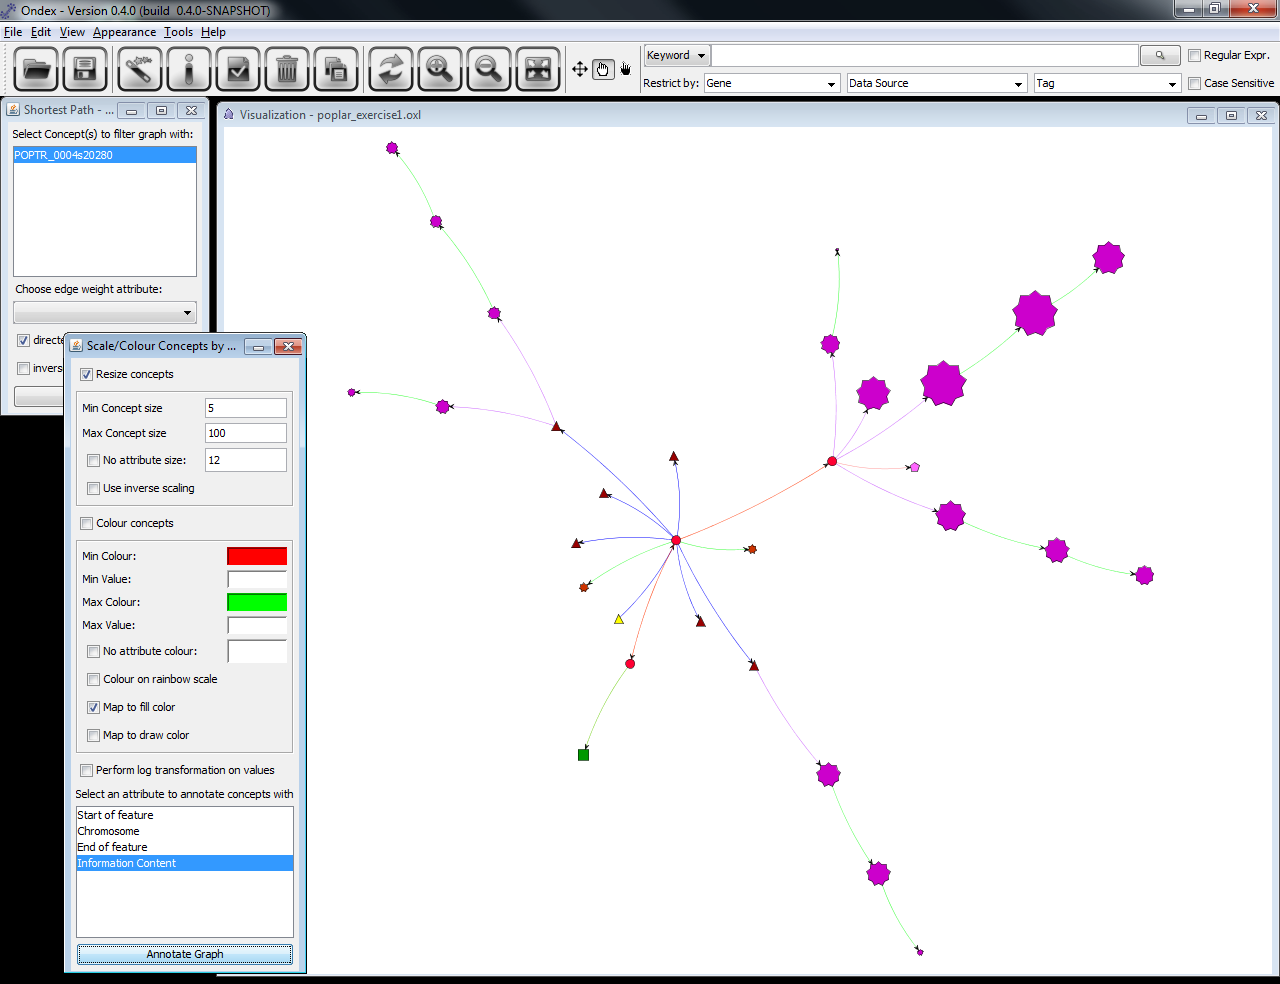
\includegraphics[scale=0.3]{images/Jun12/poplar_result_ex2_annIC.png} 
\caption{Screen-shot after annotating GO terms with their information content}
\label{fig:poplar_result_annIC}
\end{figure}

\emph{Help:}
	\begin{itemize}
	\item Hide all biological processes by clicking on one of them, right-click Hide -$>$ Same Concept Class.
	\item Apply the Gem layout again (Appearance -$>$ Layouts -$>$ Gem)
	\item Tools -$>$ Annotators -$>$ Scale/Colour Concepts by Numerical Value
	\item Select the check-box ``No attribute size'' to specify a default value for concepts which do not hold an ``Information Content'' attribute
	\item Change the sizes to 5, 100 and 5 (or experiment by yourself)
	\item Do not select ``Colour Concepts'' (we want to keep the colour as set by concept class colour legend)
	\item Select ``Information Content'' in the list of attributes available
	\item Click on ``Annotate Graph''
	\end{itemize}
\end{itemize}

%%%%%%%%%%%%%%%%%%%%%%%%%%%%%%%%%%%%%%%%%%%%%%%%%%%%%%%%%%%%%%%%%%%%%%%%%%%%%
\subsection{Exercise}
\label{sec:analysing_exercise}
Given a trait ontology term (``shoot branching'') we wish to show all Poplar proteins which are related to it in the network. 
\begin{itemize}
\item Close all the windows you have opened in Ondex (View -$>$ Windows -$>$ Close All).
\item Go to File -$>$ Open  (or click on the first button in the icon bar)
\item You should see an Open File Dialog
\item Open the Tutorial\_files/Main\_part folder, select poplar\_exercise2.oxl and click on open
\end{itemize}

\emph{Help:}
\begin{itemize}
\item Search for ``shoot branching'' in the search bar and restrict your search to the concept class ``Trait Ontology''
\item One result gets displayed. Select it and a neighbourhood depth of zero (to see only this concept), click ``Filter Graph'' and observe Figure \ref{fig:poplar_ex2_searchres}
\begin{figure}[H]
\centering
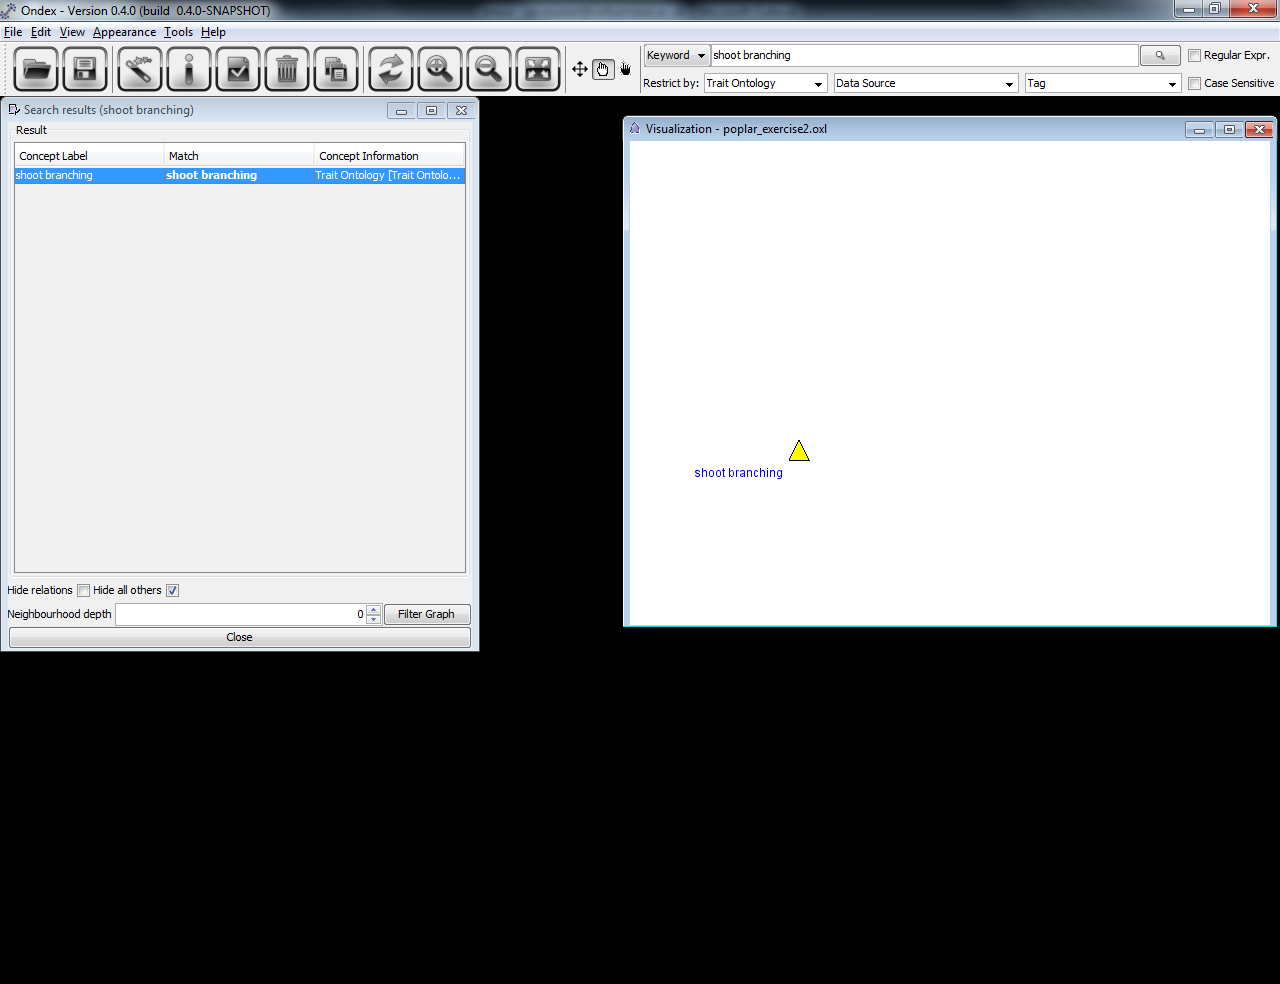
\includegraphics[scale=0.3]{images/Jun12/poplar_ex2_searchres.png} 
\caption{Screen-shot after using the embedded neighbourhood filter from the search results window}
\label{fig:poplar_ex2_searchres}
\end{figure}

\item Right-click -$>$ Show ``Immediate Neighbours by Relation Type''. 
The only one available is cooccurs\_with and will display 94 relations showing the result of the Ondex text-mining plugin (which is part of the workflow to produce this graph).
This ``shoot branching'' term cooccurs with proteins and other traits in some publications' abstracts.

\item Tools -$>$ Annotators -$>$ Scale/Colour Relations by Numerical Value
\item Select the attribute called ``Inner product of TFIDF'' in the list at the bottom
TFIDF is a measure used to evaluate how important a word is to a document in a collection or corpus (see \url{http://en.wikipedia.org/wiki/Tf-idf}).
A publication explaining the text mining module in Ondex is available at \url{http://journal.imbio.de/article.php?aid=121}.

\item Press Control A while the Visualization window is in focus to select all visible concepts in the graph
\item Right-click -$>$ Show ``Immediate Neighbours by Relation Type'' and select ``has\_similar\_sequence''
\item 91 Poplar proteins are added
\item Tools -$>$ Annotators -$>$ Scale/Colour Relations by Numerical Value
\item Tick the ``Preserve non-matching relations'' option (so that the results of the first annotator are kept)
\item Select the attribute called ``Bit Score'' in the list at the bottom
\end{itemize}

Following the cooccurs\_with relation whose width scaled up the most leads to the NCED8 (MAX4) protein in {\it{Arabidopsis}} then to POPTR\_0018s08010 and POPTR\_0006s25490 in poplar as illustrated on the screen-shot \ref{fig:poplar_ex2_searchresAnno}.
Furthermore, Ondex also offers the possibility of calling external Web services.
For example, in this case you could select these three proteins and run ClustalW using JalView.
You would need to select the three proteins, right-click -$>$ Link -$>$  Perform multiple-sequence alignment.
Once JalView is loaded up, go to Web Service -$>$ Alignment. 
\emph{Note:} other functions are available from the JalView menu ({\it{e.g.}}, calculate a phylogenetic tree).

\begin{figure}[H]
\centering
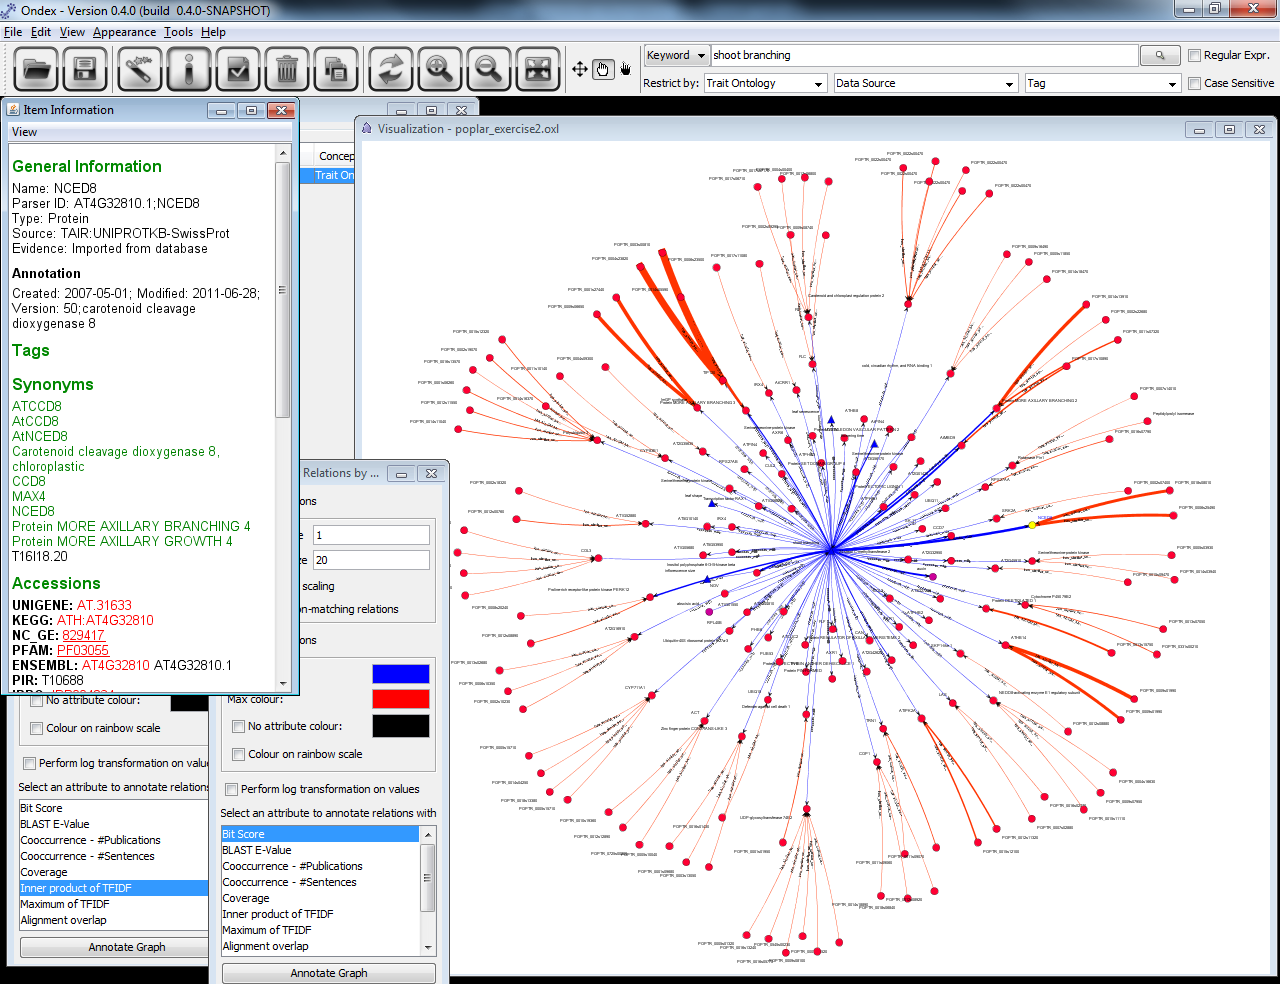
\includegraphics[scale=0.3]{images/Jun12/poplar_ex2_searchresAnno.png} 
\caption{Screen-shot after applying the Scale/Colour Relations by Numerical Value annotators}
\label{fig:poplar_ex2_searchresAnno}
\end{figure}
 % 1 Data visualisation
\chapter{Data integration}
\label{cha:integration}

Ondex front-end is used to visualize networks produced by running an Ondex workflow. 
Originally, the data integration was done by writing a workflow in XML format and by running within the Ondex back-end. 
In the following section, we are going to introduce the Ondex Integrator, which allows users to prepare and run an Ondex workflow using an intuitive GUI 
(for more information see Section \ref{sec:ref_integrator}).
Typically, a simple example for a workflow would be to first select parsers (to import data), then to select mapping methods, 
some filtering methods to improve the quality of the graph and, finally, an export method ({\it{e.g.}}, OXL export for the Ondex file format).


%%%%%%%%%%%%%%%%%%%%%%%%%%%%%%%%%%%%%%%%%%%%%%%%%%%%%%%%%%%%%%%%%%%%%%%%%%%%%%%%%%%%%%%%%%%%%%%%%%%%%%%%%%%%%%%%%%%%%%%%%%%%%%%%%%%%%%%%%%%%%%%%%%%%%%%%%%
\section{Using Ondex Integrator}
\label{sec:integrator}

The Ondex Integrator is available from Tools -$>$ Integrator in the menu of Ondex. 
Figure \ref{fig:integrator} shows it when it first opens up.
For each category showing in the left pane, stable plugins will be displayed by default.
To browse more plugins (when experimental plugins have been selected during installation), 
please untick the option ``Show stable plugins only" in the Configure menu of the Integrator.
As explained above, composing a workflow using the Integrator will require selecting various steps or Ondex plugins -
each of which offer parameters to be set if needed.
N.B.: Grayed out parameters are optional. 

\subsection{Using Ondex Integrator - an Exercise}
\label{sec:integrator_exercise}

\begin{figure}[H]
\centering
\subfigure[Botrytis Cinerea on grape]{
	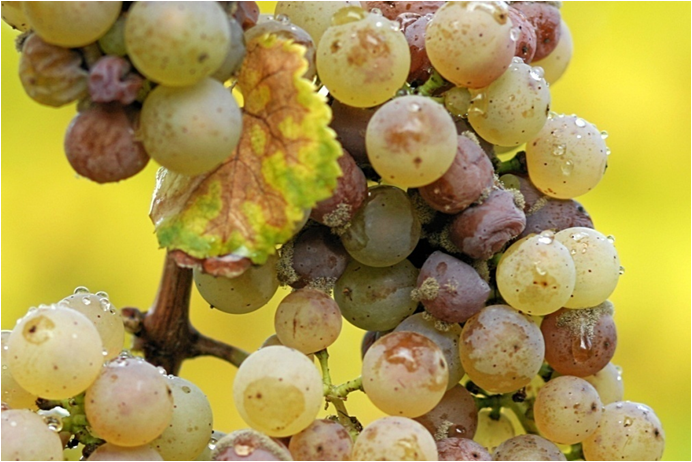
\includegraphics[scale=0.4]{images/Oct12/grape.png} 
	\label{fig:grape}
}
\subfigure[Botrytis Cinerea on strawberry]{
	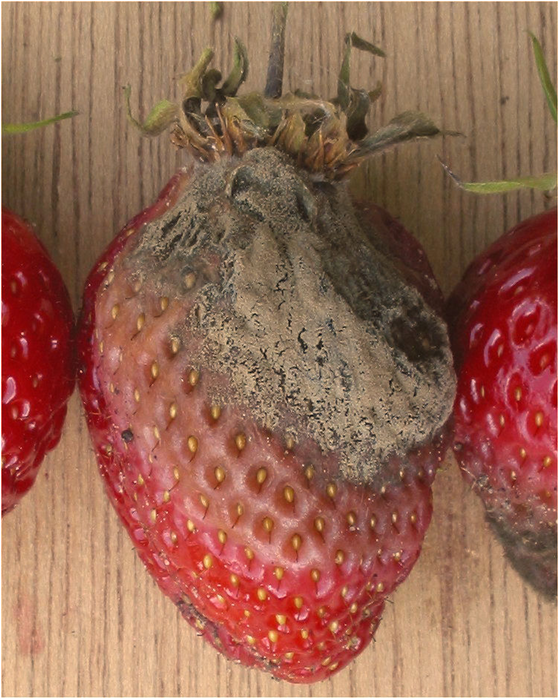
\includegraphics[scale=0.4]{images/Oct12/strawberry.png} 
	\label{fig:strawberry}
}
\label{fig:bot_in_action}
\caption{Botrytis Cinerea}
\end{figure}

\textit{Botrytis cinerea} (\url{http://www.broad.mit.edu/annotation/genome/botrytis_cinerea/}) is a necrotrophic fungus that affects many plant species. 
Its most notable hosts are wine grapes (see Figure \ref{fig:grape}) and strawberries (see Figure\ref{fig:strawberry}). 
Genomic data are available for this fungus, however we do not have much phenotypic data related to genes.
The PHI-base database (\url{http://www.phi-base.org/}) is a reference database of virulence and pathogenicity genes validated by gene disruption experiments. 
It contains information on experimentally verified pathogenicity, virulence and effector genes from bacterial, 
fungal and Oomycete pathogens identified from the scientific literature. 

For this example, techniques of comparative genomics were combined with data integration methods to predict pathogenicity genes in pathogenic organisms. 
The InParanoid algorithm\footnote{Remm M., Storm C.E., Sonnhammer E.L. (2001). 
``Automatic clustering of orthologs and in-paralogs from pairwise species comparisons''. Journal of Molecular Biology, 314(5):1041-52, PubMed ID: 11743721.}
was implemented as part of the Ondex system for the prediction of orthologous groups of proteins.
The workflow we are working on in this section is illustrated in Figure \ref{fig:phi_bot}.

\begin{figure}[H]
\centering
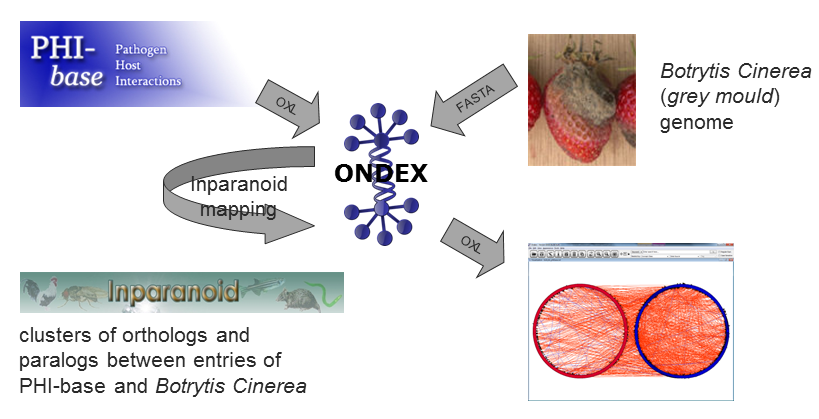
\includegraphics[scale=0.5]{images/Oct12/integration_phi_bot.png} 
\caption{Integrating PHI-base and genomic information of \textit{Botrytis Cinerea}}
\label{fig:phi_bot}
\end{figure}


\begin{figure}[H]
\centering
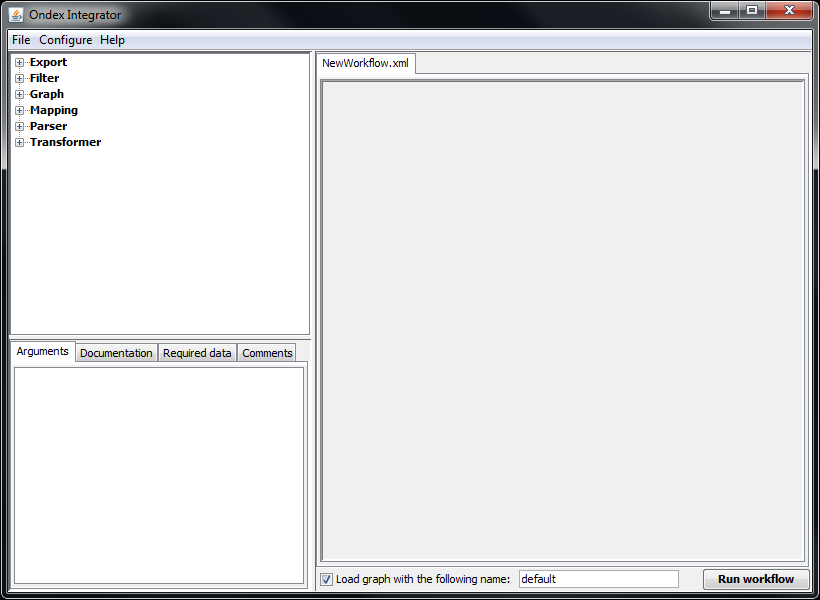
\includegraphics[scale=0.5]{images/Oct12/integrator.png} 
\caption{Data integration using the graphical interface - Ondex Integrator}
\label{fig:integrator}
\end{figure}


Note: Running this workflow with the whole genome sequence from \textit{Botrytis} will take about an hour. 
If you wish to see quick results during this hands-on tutorial, we suggest you use a FASTA file which has been prepared for this purpose: 
short.fasta which can be found under Tutorial\_files/Data\_integration/Integrator. 
This file contains a tenth of the entire genome and will take about 3 minutes. 
The results show a smaller graph which can be analysed nevertheless. 
In Chapter \ref{cha:comp}, we will load up the results for the whole genome and study them using
Ondex annotators (these results are saved under Tutorial\_files/Application\_cases/botrytis\_phibase.oxl).

Note: Before running a workflow in the Ondex Integrator, make sure you save your current workflow 
so you can re-open it as you might not get all the parameters right the first time around.
For this example, the steps needed in the workflow are as follows
({\em{All the files needed here are saved under Tutorial\_files/Data\_integration/Integrator}}):

\begin{itemize}
\item Parsing the file containing the PHI-base database (Parser - OXL Parser, see Figure \ref{fig:integrator_oxlimport}). 
Note: A ``New memory graph'' pre-step is automatically loaded.
\begin{figure}[H]
\centering
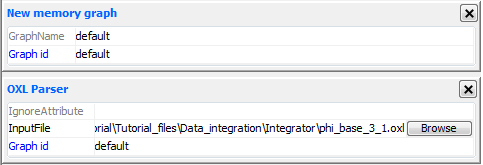
\includegraphics[scale=0.6]{images/Oct12/oxlimport.png} 
\caption{Parser - OXL Parser}
\label{fig:integrator_oxlimport}
\end{figure}
Opening this OXL file directly would produce the metagraph shown in Figure \ref{fig:metagraph_phibase}.
\begin{figure}[H]
\centering
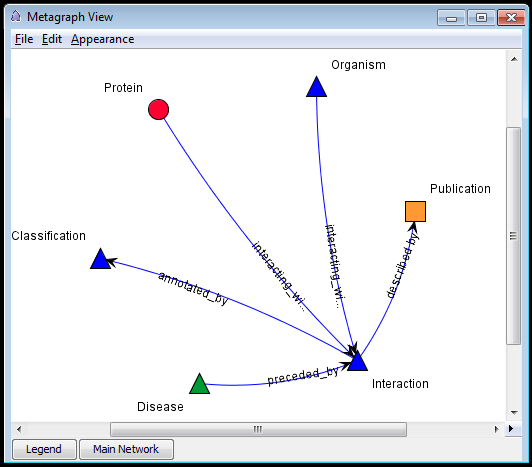
\includegraphics[scale=0.6]{images/Oct12/phibase.png} 
\caption{Metagraph - PHI-base}
\label{fig:metagraph_phibase}
\end{figure}
If you have time, have a look at the main graph. 
In particular, try to find which concepts hold the phenotypic information we are actually interested in for this workflow.
This will later determine which concept classes you can filter out, which ones you should keep and/or combine.

\item Parsing the file downloaded from the Broad institute website for the sequence of \textit{Botrytis Cinerea} 
(Parser - FASTA file parser, see Figure \ref{fig:integrator_fasta})
Note: The taxonomy ID for \textit{Botrytis Cinerea} was found on \url{http://www.ncbi.nlm.nih.gov/taxonomy/} (40559). 
CC stands for Concept Class and is therefore ``Protein''. 
SeqType stands for Sequence Type and is in this case ``AA'', amino acid.
\begin{figure}[H]
\centering
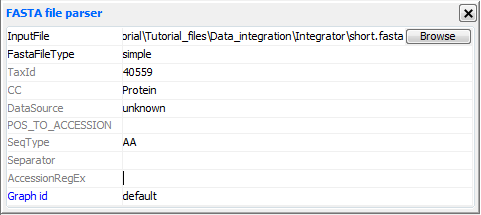
\includegraphics[scale=0.6]{images/Oct12/fasta.png} 
\caption{Parser - FASTA file parser}
\label{fig:integrator_fasta}
\end{figure}
An export (select Export in the left-hand information tree and OXL Export in the list of exporters) at the end of a workflow
containing only the FASTA file parser would produce the metagraph shown in Figure \ref{fig:metagraph_botrytis}.
\begin{figure}[H]
\centering
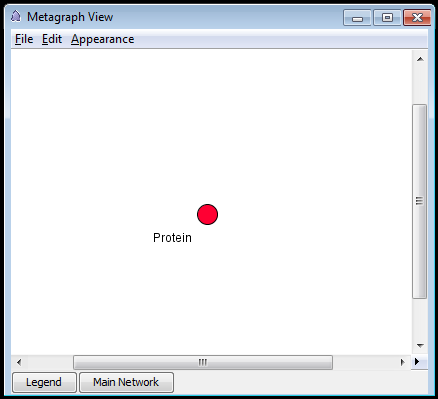
\includegraphics[scale=0.6]{images/Oct12/botrytis.png} 
\caption{Metagraph - Botrytis}
\label{fig:metagraph_botrytis}
\end{figure}

\item After parsing the two data sources, they are mapped to each other using the ``Inparanoid'' mapping which uses pair-wise sequence alignment results 
generated by BLAST \url{http://www.ncbi.nlm.nih.gov/books/NBK1762/} (Mapping - Inparanoid, see Figure \ref{fig:integrator_inparanoid}). 
The ``Evalue'' parameter is passed on to BLAST.
``Cutoff'' and ``Overlap'' are post filter parameters which specify a bit score cutoff and the minimum length of the match compared to the longest sequence.
({\em{If BLAST is not installed on your machine, please download the appropriate installer from 
\url{ftp://ftp.ncbi.nlm.nih.gov/blast/executables/blast+/LATEST/} 
The Inparanoid mapping method expects to be given the bin directory of your BLAST installation.}})
\begin{figure}[H]
\centering
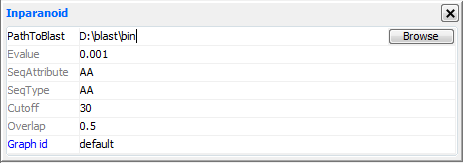
\includegraphics[scale=0.6]{images/Oct12/inparanoid.png} 
\caption{Mapping - Inparanoid}
\label{fig:integrator_inparanoid}
\end{figure}
An export at this stage would produce the metagraph shown in Figure \ref{fig:inparanoid_results}.
\begin{figure}[H]
\centering
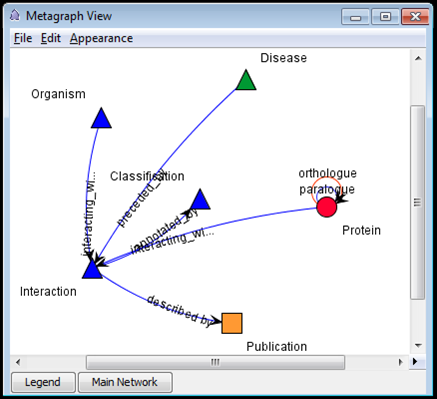
\includegraphics[scale=0.6]{images/Oct12/inparanoid_results.png} 
\caption{Metagraph - Results of the Inparanoid mapping method}
\label{fig:inparanoid_results}
\end{figure}

\item To reduce the complexity of the network several concept classes we are not interested in are filtered out
(Filter - ConceptClass Filter, see Figure \ref{fig:integrator_cc}).
\begin{figure}[H]
\centering
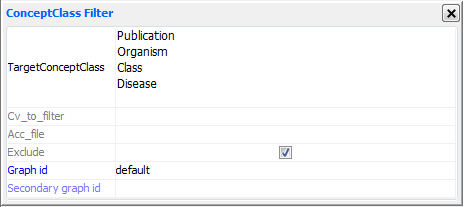
\includegraphics[scale=0.6]{images/Oct12/cc.png} 
\caption{Filter - ConceptClass Filter}
\label{fig:integrator_cc}
\end{figure}

\item In PHI-base a concept of class ``Protein'' is always linked to an ``Interaction'' which carries the specific phenotype. 
To merge both information from ``Protein'' and ``Interaction'' the relation type ``int\_w'' is collapsed and 
the connected concepts are merged into a single concept of concept class ``Interaction:Protein''. 
(Transformer - Relation Collapser, see Figure \ref{fig:integrator_relationCollapser})
\begin{figure}[H]
\centering
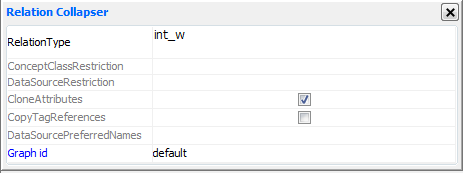
\includegraphics[scale=0.6]{images/Oct12/relationCollapser.png} 
\caption{Transformer - Relation Collapser}
\label{fig:integrator_relationCollapser}
\end{figure}
An export at this stage would produce the metagraph shown in Figure \ref{fig:intermediate_results}.
\begin{figure}[H]
\centering
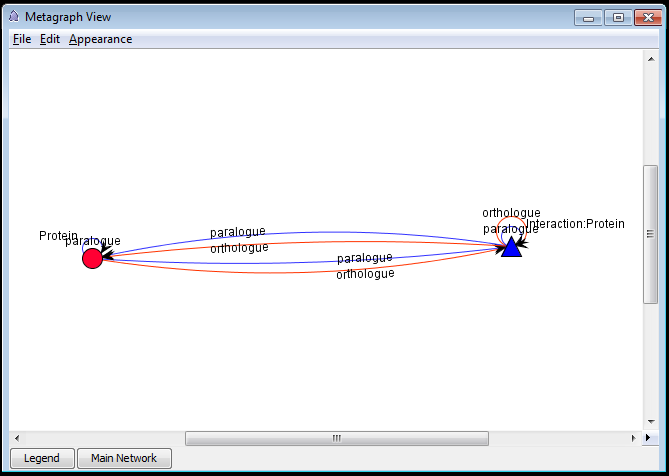
\includegraphics[scale=0.6]{images/Oct12/intermediate_results.png} 
\caption{Metagraph - Results of the ConceptClass Filter and the Relation Collapser}
\label{fig:intermediate_results}
\end{figure}

\item An export at this stage would produce the graph shown in Figure \ref{fig:need_unconnected}.
\begin{figure}[H]
\centering
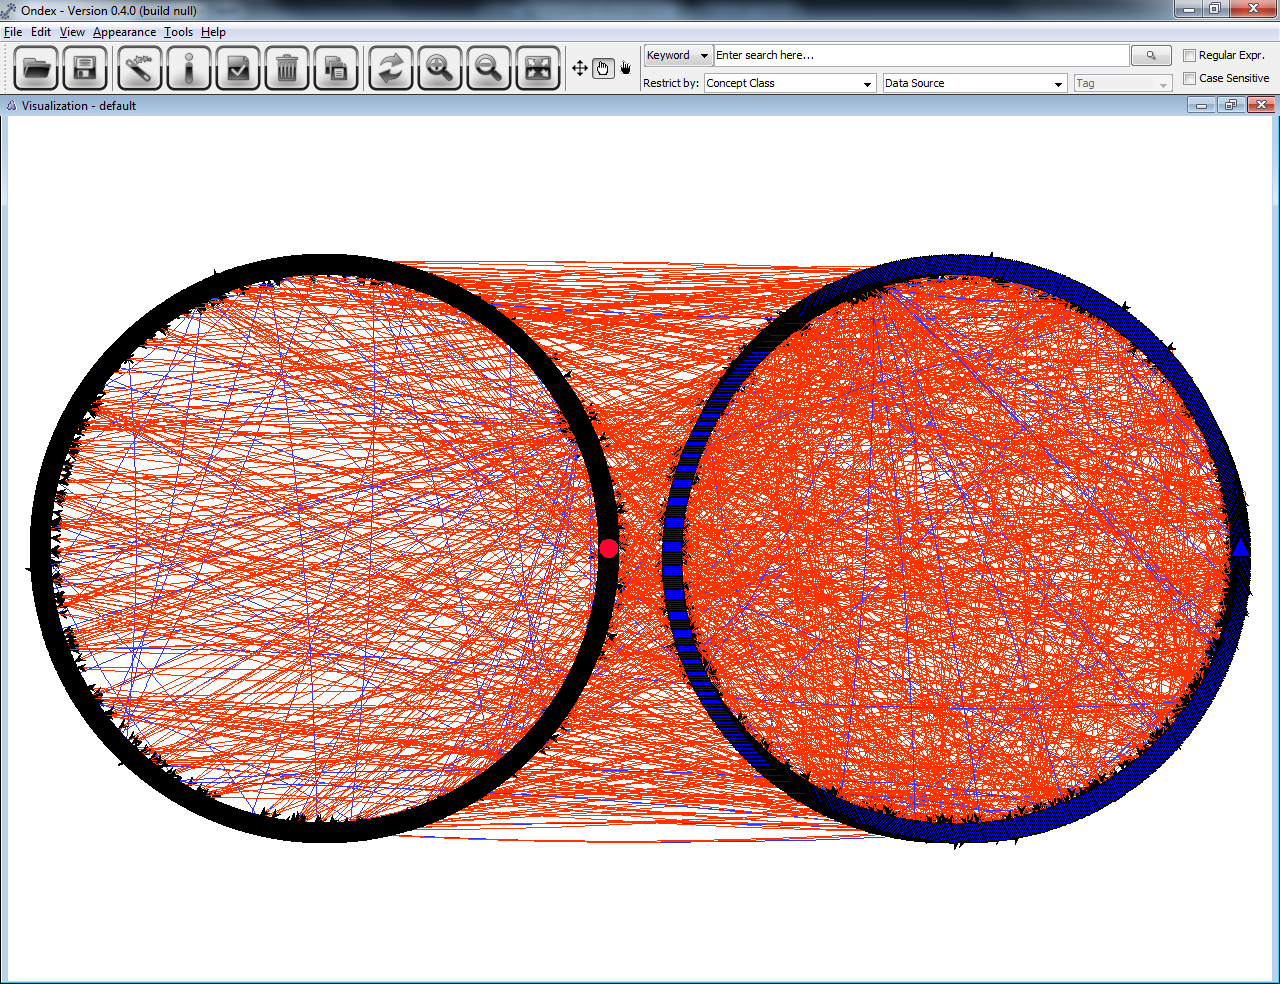
\includegraphics[scale=0.3]{images/Oct12/need_unconnected.png} 
\caption{Main graph - Need for the Unconnected Filter}
\label{fig:need_unconnected}
\end{figure}
The Unconnected Filter is used to remove any isolated concepts (i.e. without any relations to the rest of the network).
(Filter - Unconnected Filter, see Figure \ref{fig:integrator_unconnected})
\begin{figure}[H]
\centering
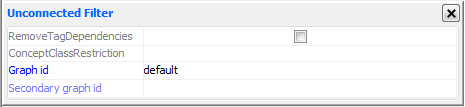
\includegraphics[scale=0.6]{images/Oct12/unconnected.png} 
\caption{Filter - Unconnected Filter}
\label{fig:integrator_unconnected}
\end{figure}

\item An export at this stage would contain the graphs shown in Figure \ref{fig:clusters}.
\begin{figure}[H]
\centering
\subfigure[Main graph - Example of a cluster of interest]{
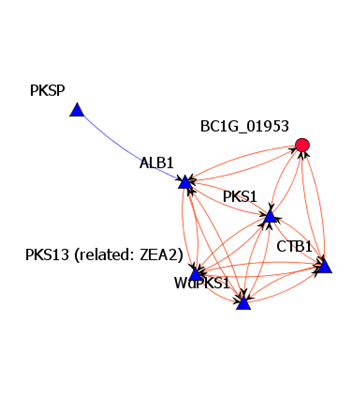
\includegraphics[scale=0.6]{images/Oct12/need_clusters_good.png} 
\label{fig:cluster_good}
}
\subfigure[Main graph - Example of a cluster we wish to remove]{
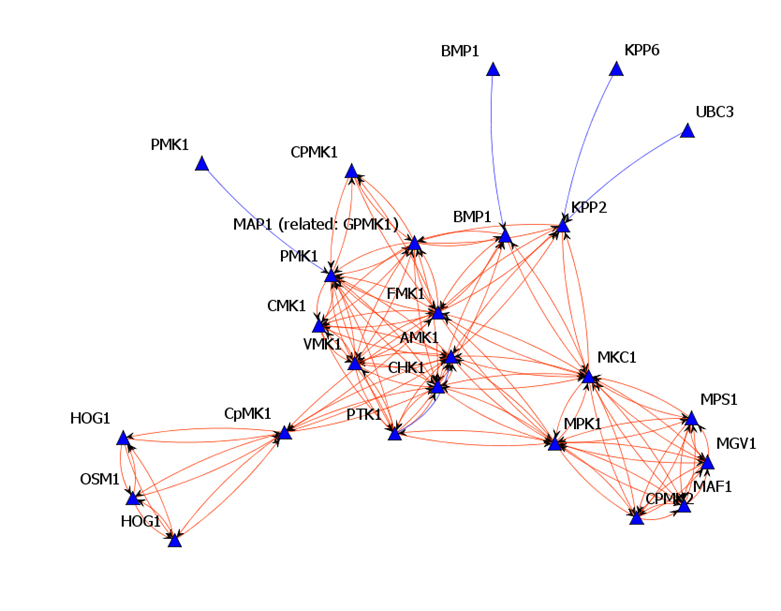
\includegraphics[scale=0.6]{images/Oct12/need_clusters_bad.png} 
\label{fig:cluster_bad}
}
\label{fig:clusters}
\caption{Two kinds of resulting clusters}
\end{figure}
Therefore the next step will only keep clusters of concepts in the network which contain at least one concept of concept class ``Protein'' 
from \textit{Botrytis Cinerea}. 
(Filter - IsolateClusters Filter, available in the experimental package - please untick the option in the Configure menu of the Ondex Integrator,
see Figure \ref{fig:integrator_isolateclusters})
\begin{figure}[H]
\centering
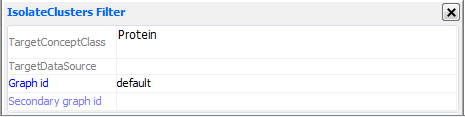
\includegraphics[scale=0.6]{images/Oct12/isolateclusters.png} 
\caption{Filter - Isolateclusters}
\label{fig:integrator_isolateclusters}
\end{figure}

\item The resulting network is exported as OXL (Export - OXL Export, see Figure \ref{fig:integrator_oxlexport}) to an Ondex network file called short\_botrytis\_results.oxl
\begin{figure}[H]
\centering
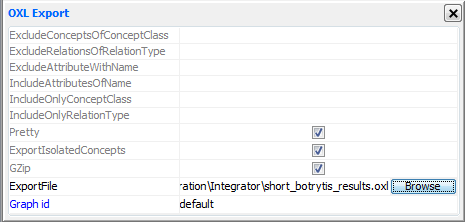
\includegraphics[scale=0.6]{images/Oct12/oxlexport.png} 
\caption{Export - OXL Export}
\label{fig:integrator_oxlexport}
\end{figure}

\end{itemize}
Loading short\_botrytis\_results.oxl in Ondex will look similar to Figure \ref{fig:phi_bot_results}.
\begin{figure}[h]
\centering
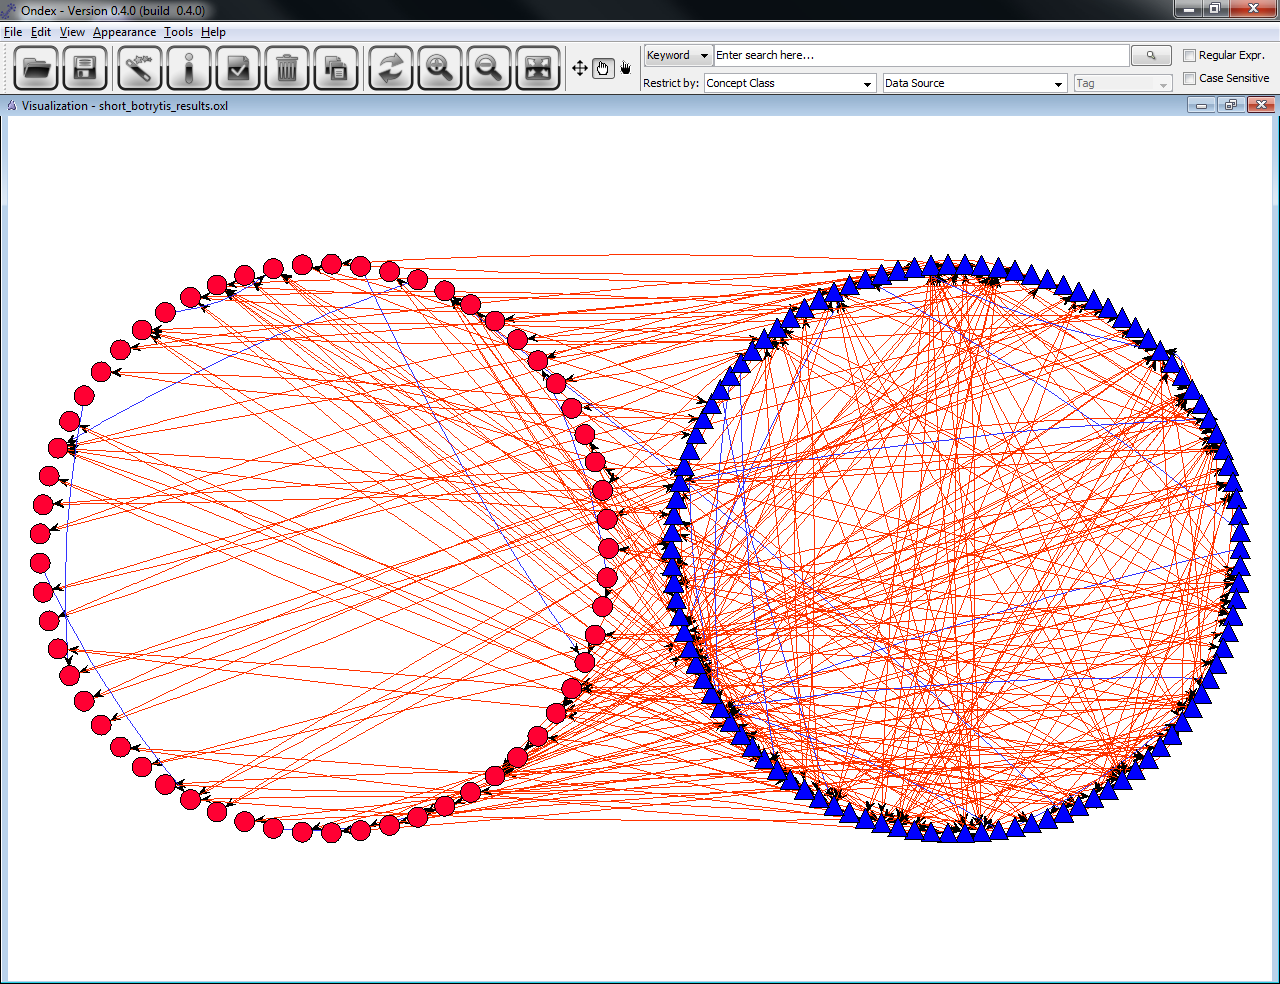
\includegraphics[scale=0.3]{images/Oct12/short_botrytis_results.png} 
\caption{Resulting graph after integration}
\label{fig:phi_bot_results}
\end{figure}




%%%%%%%%%%%%%%%%%%%%%%%%%%%%%%%%%%%%%%%%%%%%%%%%%%%%%%%%%%%%%%%%%%%%%%%%%%%%%%%%%%%%%%%%%%%%%%%%%%%%%%%%%%%%%%%%%%%%%%%%%%%%%%%%%%%%%%%%%%%%%%%%%%%%%%%%%%
\section{Using the scripting console}
\label{sec:parsing_tabdel}
When Ondex does not provide any specific parser for the data a user is interested and this data is in a tab delimited format, 
it is possible to use a general tab delimited parser. This section explains how to use it.

\subsection{Basic functionality and parsing of delimited files}
The prototype based parsing API aims to simplify and speed up the import of user defined formats into Ondex graphs. 
As custom formats are highly variable it is impossible to write a universal parser to deal with all of the possible options. 
This approach aims to provide the middle ground way that retains all of the flexibility but takes care of the complexity involved 
with using the Ondex JAVA API directly. Most delimited files can be parsed in about 5 lines. 
The following guide is primarily for using the API through the scripting interface, although it can be used directly from JAVA as well.

Steps for example 1 (explained below):
\begin{itemize}
\item Open a new empty graph
\item Tools -$>$ Console
\item Type commands in the console or copy and paste the prepared script available at Tutorial\_files/Data\_integration/Console/readme\_scripting.txt
(change the path to test.tab so that it points to the correct file, make sure to keep forward slashes)
\item Press enter (a quarter of a concept should appear in the top-left corner)
\item Appearance -$>$ Layouts -$>$ Gem
\end{itemize}

\textbf{Example 1}
The tab-delimited file in Figure \ref{fig:tab_and_graph} produces the network on its right-hand side (using the commands underneath).
\begin{figure}[h]
\centering
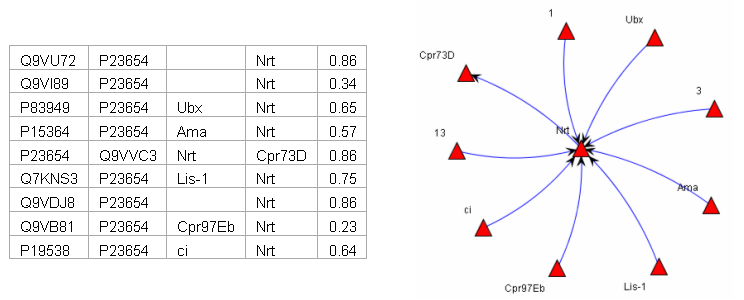
\includegraphics[scale=0.5]{images/Oct12/tab_and_graph.png} 
\caption{Tab-delimited file and generated graph}
\label{fig:tab_and_graph}
\end{figure}


\begin{verbatim}
p = new PathParser(getActiveGraph(), 
	new DelimitedFileReader("C:/test.tab", "	"));
\end{verbatim}
This statement creates a new parser. The ``getActiveGraph()'' method call gives the reference to the last active visualisation frame in Ondex (at least one must be open). 
The ``DelimitedFileReader" takes a path to the file and a delimiter (in this case tab) as an argument.
\begin{verbatim}
c1 = p.newConceptPrototype(
	defAccession(0, "UNIPROTKB"), defCC("Protein"), defName(2));
c2 = p.newConceptPrototype(
	defAccession(1, "UNIPROTKB"), defCC("Protein"), defName(3));
\end{verbatim}
Here new concept prototypes are added to the parser. This method can take any number of arguments in any order. 
The arguments specify which user data (or which column) will be converted to which argument. 
In the above example, the integers 0, 1, 2, 3 represent the number of the column where the information can be found.
\begin{verbatim}
p.newRelationPrototype(
	c1, c2, defAttribute(4, "P-value", "NUMBER"));
\end{verbatim}
This statement creates a relation prototype that will create a relation between the two concepts created from the prototypes ``c1'' and ``c2''. 
The source and target concepts are the only two required arguments. There can be any number of relation attribute arguments that can be in any order.
Attributes get specified using ``defAttribute''.
\begin{verbatim}
p.parse();
\end{verbatim}
Parses the file and creates the graph.

\vspace{1cm}
\textbf{Example 2}
\begin{verbatim}
p = new PathParser(getActiveGraph(), new DelimitedFileReader
("D:/workspace/core/data/importdata/Uniprot2AGI.tab", "	"));
p.newConceptPrototype(defCC("Protein"), 
	defAccession(0, "UNIPROTKB"), defAccession(1, "TAIR"));
p.setProcessingOptions();
\end{verbatim}
Sets the processing options to none - by default the concepts created will always be merged on accessions, 
but the parsing process will take much longer - even if no concepts actually satisfy this requirement.
\begin{verbatim}
p.parse();
\end{verbatim}

\textbf{Attribute specification arguments}
All attribute specification arguments are optional and can be supplied in any order. 
The type of the argument corresponds to the name of the function and the first argument is always either a position in the data vector 
(\textit{e.g.} column in the case of tab delimited files) or a String (in double quotes) when it is desired to have an argument as a constant value, 
rather than have it parsed from the data file.



\subsection{Concepts and Relations}
The diagram \ref{fig:script_concepts_relations} below outlines the data structure of an Ondex concept and an Ondex relation. 
Fields in green hold actual data, whereas fields in blue are compound attributes that group sub-attributes of their own. 
Three overlaid attribute boxes indicate that multiple instances of attributes of this type can exist. 
Attributes represent a special case because any number of attributes may exist as long as the attribute name specified for each of them is unique. 
The boxes with dashed outline are Boolean values that should be specified as Strings "true" and "false".

The only required parameter is the first one that can be either an Integer or String, the rest of the parameters are optional. 

\textbf{Attribute types}
The valid options are: 
\begin{verbatim}"NUMBER", "TEXT", "INTEGER", "COLOR", "DOUBLE" and "OBJECT"\end{verbatim}
\textit{e.g.:} 
\begin{verbatim}defAttribute("3.14", "Pi", "NUMBER");\end{verbatim}

\textbf{Processing options}
To specify that no processing options should be applied, set empty processing options:
\begin{verbatim}p.setProcessingOptions();\end{verbatim}
Disabling the post-processing options will increase the parsing speed considerably. 
The following processing options are available, from none to all three may be set at the same time: 
\begin{verbatim}"MERGE_ON_ACCESSIONS"\end{verbatim} (on by default)
\begin{verbatim}"MERGE_ON_NAMES"\end{verbatim}
\begin{verbatim}"MERGE_ON_ATTRIBUTE"\end{verbatim}

Accessions supported by Ondex are listed in Appendix \ref{cha:accessions}.

Relation types supported by Ondex are listed in Appendix \ref{cha:relation_types}.

\begin{figure}[H]
\centering
\subfigure[Data structure of an Ondex concept]{
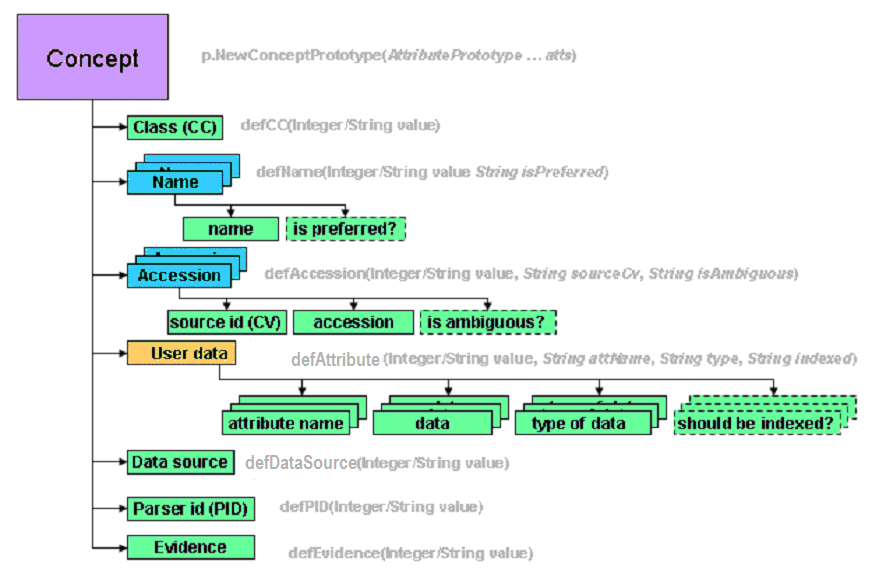
\includegraphics[scale=0.6]{images/Oct12/script_concept.png} 
\label{fig:script_concepts}
}
\subfigure[Data structure of an Ondex relation]{
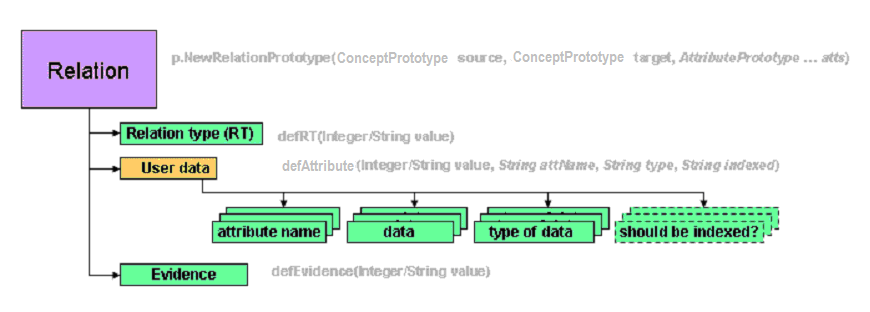
\includegraphics[scale=0.6]{images/Oct12/script_relation.png} 
\label{fig:script_relations}
}
\label{fig:script_concepts_relations}
\caption{Ondex data structure}
\end{figure}

\newpage
%%%%%%%%%%%%%%%%%%%%%%%%%%%%%%%%%%%%%%%%%%%%%%%%%%%%%%%%%%%%%%%%%%%%%%%%%%%%%%%%%%    
\section{Accession based mapping examples}
\label{sec:accmapping_examples}
This section illustrates how accession based mapping works with examples.

\subsection{No parameters}
\begin{center}
\begin{tabular}{|c|c|c|c|}\hline
Name & Concept Class & Data Source & Accession\\ \hline			
P1 & Protein & UNIPROTKB & UNIPROTKB:ACC1\\
P2 & Protein & TAIR & UNIPROTKB:ACC1\\
\hline  
\end{tabular}
\end{center}
\vspace{0.5cm}
P1 and P2 will map with no parameters needed because this mapping method maps concepts of the same concept class (Protein) and of different data source (UNIPROTKB and TAIR).

\subsection{EquivalentConceptClass parameter}
\begin{center}
\begin{tabular}{|c|c|c|c|}\hline
Name & Concept Class & Data Source & Accession\\ \hline			
P1 & Protein & UNIPROTKB & UNIPROTKB:ACC1\\
G1 & Gene & TAIR & UNIPROTKB:ACC1\\
\hline  
\end{tabular}
\end{center}
\vspace{0.5cm}
P1 and G1 will map if parameter EquivalentConceptClass is set to "Protein,Gene", so that the mapping method recognises these two concept classes as equivalent.

\subsection{EquivalentCV parameter (equivalent accession type)}
\begin{center}
\begin{tabular}{|c|c|c|c|}\hline
Name & Concept Class & Data Source & Accession\\ \hline			
P1 & Protein & UNIPROTKB & UNIPROTKB:ACC1\\
P2 & Protein & TAIR & TAIR:ACC1\\
\hline  
\end{tabular}
\end{center}
\vspace{0.5cm}
P1 and P2 will map if parameter EquivalentCV is set to "UNIPROTKB,TAIR", so that the mapping method recognises these two accession types as equivalent.

\subsection{WithinCVMapping parameter (within data source)}
\begin{center}
\begin{tabular}{|c|c|c|c|}\hline
Name & Concept Class & Data Source & Accession\\ \hline			
P1 & Protein & UNIPROTKB & UNIPROTKB:ACC1\\
P2 & Protein & UNIPROTKB & UNIPROTKB:ACC1\\
\hline  
\end{tabular}
\end{center}
\vspace{0.5cm}
P1 and P2 will map if parameter WithinCVMapping is set to true, so that the method maps concepts of the same concept class and same data source.

\subsection{IgnoreAmbiguity parameter (use ambiguous accessions)}
\begin{center}
\begin{tabular}{|c|c|c|c|c|}\hline
Name & Concept Class & Data Source & Accession & Ambiguous\\ \hline			
P1 & Protein & UNIPROTKB & UNIPROTKB:ACC1 & false\\
P2 & Protein & TAIR & UNIPROTKB:ACC1 & true\\
\hline  
\end{tabular}
\end{center}
\vspace{0.5cm}
P1 and P2 will map if the parameter IgnoreAmbiguity is set to true, so that the mapping method ignores the P2's ambiguous flag.

\subsection{ConceptClassRestriction parameter}
\begin{center}
\begin{tabular}{|c|c|c|c|}\hline
Name & Concept Class & Data Source & Accession\\ \hline			
P1 & Protein & UNIPROTKB & UNIPROTKB:ACC1\\
P2 & Protein & TAIR & UNIPROTKB:ACC1\\
G1 & Gene & UNIPROTKB & UNIPROTKB:ACC1\\
G2 & Gene & TAIR & UNIPROTKB:ACC1\\
\hline  
\end{tabular}
\end{center}
\vspace{0.5cm}
If no parameters are specified, two relations will be created: one between the two genes and one between the two proteins.
If the parameter ConceptClassRestriction is set to Protein, only the two proteins will be mapped.

\subsection{CVRestriction parameter (accession type restriction)} 
\begin{center}
\begin{tabular}{|c|c|c|c|}\hline
Name & Concept Class & Data Source & Accession\\ \hline			
P1 & Protein & UNIPROTKB & UNIPROTKB:ACC1\\
P2 & Protein & UNIPROTKB & TAIR:ACC1\\
P3 & Protein & TAIR & UNIPROTKB:ACC1\\
P4 & Protein & TAIR & TAIR:ACC1\\
\hline  
\end{tabular}
\end{center}
\vspace{0.5cm}
If no parameters are specified, two relations will be created: one between P1 and P3, and one between P2 and P4.
If the parameter CVrestriction is set to TAIR, only P2 and P4 will be mapped.

\subsection{WithinCVMapping parameter (within data source) and EquivalentCV parameter (equivalent accession type)} 
\begin{center}
\begin{tabular}{|c|c|c|c|}\hline
Name & Concept Class & Data Source & Accession\\ \hline			
P1 & Protein & UNIPROTKB & UNIPROTKB:ACC1\\
P2 & Protein & UNIPROTKB & TAIR:ACC1\\
\hline  
\end{tabular}
\end{center}
\vspace{0.5cm}
P1 and P2 will be mapped if WithinCVMapping is set to true and EquivalentCV is set to "UNIPROTKB,TAIR".


%%%%%%%%%%%%%%%%%%%%%%%%%%%%%%%%%%%%%%%%%%%%%%%%%%%%%%%%%%%%%%%%%%%%%%%%%%%%%%%%%%    
\section{Exercise}
Open file Tutorial\_files/Data\_integration/Exercise/exercise.tab in a text editor.
\subsection{Scripting Console}
\begin{itemize}
\item Edit Data\_integration/Exercise/exercise\_scripting.txt to import the 6 concepts in exercise.tab in Ondex using the scripting console.
As Section \ref{sec:parsing_tabdel} showed, the scripting console maps equivalent concepts by default and collapses them. 
For the purpose of the following exercise, exercise\_scripting.txt contains a p.setProcessingOptions() command which disables this feature.
Please use "UNIPROTKB" whenever defining "defAccession".
\item Once the scripting console has generated six concepts, save your graph.
\end{itemize}

\subsection{Integrator}
\begin{itemize}
\item Open the integrator and compose a workflow to import the graph you have just saved, 
map concepts based on their accessions (with no parameters for now) and export. 
\item Before opening your resulting graph, guess which concepts have been mapped and are now linked by new relations.
\item Come back to your workflow and experiment with parameters aiming to map:
	\begin{itemize}
	\item P2 and P4
	\item P3 and G2
	\item P1 and G1
	\end{itemize}
Do other concepts map too? Why?	
\end{itemize}

 % 2 Data integration
\chapter{GUI Reference}
\label{cha:ref}



%%%%%%%%%%%%%%%%%%%%%%%%%%%%%%%%%%%%%%%%%%%%%%%%%%%%%%%%%%%%%%%%%%%%%%%%%%%%%%%%%%%%%%%%%%%%%%%%%%%%%%%%%%%%%%%%%%%%%%%%%%%%%%%%%%%%%%%%%%%%%%%%%%%%%%%%%%
\section{Installation}
\label{sec:ref_install}

%%%%%%%%%%%%%%%%%%%%%%%%%%%%%%%%%%%%%%%%%%%%%%%%%%%%%%%%%%%%%%%%%%%%%%%%%%%%%
\subsection{Requirements}
\textbf{Hardware: }Ondex requires at least
\begin{itemize}
\item 2GHz CPU
\item 2GB RAM (4GB recommended)
\item 300 MB of free HDD space
\end{itemize}

\noindent\textbf{Operating system: }Ondex is a Java 6 application and therefore compatible with
\begin{itemize}
\item Windows XP / Vista / 7
\item Linux / UNIX / Solaris
\item Mac OS X 64-bit Intel (as this version supports Java 6)
\end{itemize}

\noindent\textbf{Software: }Ondex needs Java version 6 update 26 or later versions.
Make sure you have an adequate Java Runtime Environment installed on your system.
If not, you can download it from {\url{http://java.oracle.com}}.

Also make sure your PATH variable contains your java executable. 
To test whether this is the case, see section \ref{sec:testing_requirements} below.

%%%%%%%%%%%%%%%%%%%%%%%%%%%%%%%%%%%%%%%%%%%%%%%%%%%%%%%%%%%%%%%%%%%%%%%%%%%%%
\subsection{Installer}
There is an Ondex installer for Windows users. 
For Windows Vista / 7: Make sure NOT to install Ondex in ``C:$\backslash$Program Files (x86)''.

In the Ondex setup, the page ``Choose Components'' (see Figure \ref{fig:choose_components}) 
lets the user decide which features of Ondex they wish to install.
Several options are possible:
\begin{enumerate}
\item Ondex front-end plug-ins
\item Ondex front-end plug-ins (including experimental)
\item All Ondex front-end and Integrator plug-ins
\item All Ondex front-end and Integrator plug-ins (including experimental)
\item Custom
\end{enumerate}
The first option will allow users to use data visualisation tools which are stable.
The second option will allow users to use data visualisation tools which are stable as well as experimental.
The third option will allow users to use data visualisation and integration tools which are stable.
The fourth option will allow users to use data visualisation and integration tools which are stable as well as experimental.
The fifth option will allow users to customize their setup and manually select what they wish to install.
(For this fifth option, the plug-ins selected by default depend on what option out of the first four was last selected.)

\begin{figure}[H]
\centering
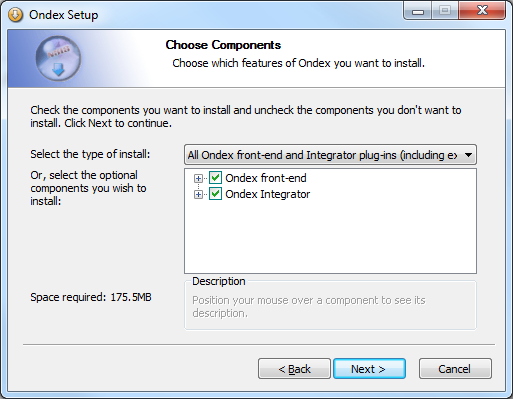
\includegraphics[scale=0.75]{images/Oct12/choose_components.png} 
\caption{Ondex Setup - Choose Components}
\label{fig:choose_components}
\end{figure}

During the installation, the Ondex setup (see figure \ref{fig:choose_memory}) 
will prompt the user to specify the default amount of memory Ondex should run with. 
This number should be set to 1200 for 32-bit systems with at least 2GB memory. 
For 64-bit systems it can be set to just under the amount of memory you have installed, 
\textit{e.g.} set it to 3500 on a system with 4GB of memory.

\begin{figure}[H]
\centering
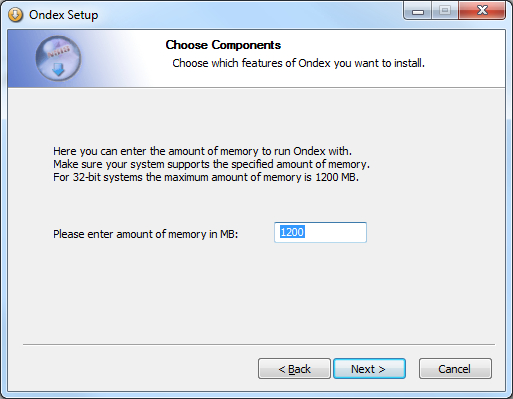
\includegraphics[scale=0.75]{images/Oct12/choose_memory.png} 
\caption{Ondex Setup - Configure memory}
\label{fig:choose_memory}
\end{figure} 

The installer will create shortcuts (which users can then access from the Start menu) unless stated otherwise during the setup.
Running the exe file for Ondex (using this shortcut or by double-clicking on it) will check that Java Runtime Environment version 1.6 or higher is installed.
If it is not, it will attempt to automatically download it.

Users of other operating systems may download the tar.gz file and execute the runme.sh file to start Ondex.
In Linux, a ``chmod 755 runme.sh'' might be needed to make the script executable from your user's account.



%%%%%%%%%%%%%%%%%%%%%%%%%%%%%%%%%%%%%%%%%%%%%%%%%%%%%%%%%%%%%%%%%%%%%%%%%%%%%
\subsection{Testing the requirements}
\label{sec:testing_requirements}

\textbf{WINDOWS: }
Click Start -$>$ Run enter ``cmd'' and press enter. 

\noindent\textbf{LINUX/GNOME: }
Right-click on your desktop and choose ``Open Terminal'' from the appearing context menu.

\noindent\textbf{LINUX/KDE: }
Choose ``Konsole'' from your Quick launcher.

Type ``java -version'' in the appearing console window and press enter.
If your system is configured correctly you will see a message that contains your current Java version. Make sure it is higher than version 1.6.
If you don't see a message, then you have either not installed Java yet, or you have not set your PATH variable.

%%%%%%%%%%%%%%%%%%%%%%%%%%%%%%%%%%%%%%%%%%%%%%%%%%%%%%%%%%%%%%%%%%%%%%%%%%%%%
\subsection{How to set the PATH variable}
\textbf{WINDOWS: }
Right-click on ``Computer'' in the start menu and choose ``Properties'' from the appearing context menu. 
Click on ``Advanced system settings'' on the left in the appearing window. 
Click the button ``Environment Variables'' on the bottom left of the window. 
You will see a list of variables with their assigned values. 
If the PATH variable already occurs in it, select it and click ``Edit''. 
Append a semicolon to the end of the value field and then enter the path to your Java binary directory. 
This is usually something like ``C:$\backslash$Program Files$\backslash$Java$\backslash$jdk1.6.0\_26$\backslash$bin''.
If the path contains any white spaces, make sure you put it in double quotes. 
If the variable PATH didn't exist yet on your system, create a new one and call it ``PATH''. 
Assign the binary path as it's value. However you don't need the semicolon in this case.

\noindent\textbf{LINUX: }
Go to your home directory and open the file ``.bashrc'' in your favourite editor. 
Append the line PATH=\$PATH:$<$javadir$>$ where $<$javadir$>$ is your path to the java binary directory, 
something like $/usr/java/latest/bin/$ to find out what it actually is you can execute the command ``type java'' in a console window. 

%%%%%%%%%%%%%%%%%%%%%%%%%%%%%%%%%%%%%%%%%%%%%%%%%%%%%%%%%%%%%%%%%%%%%%%%%%%%%
\subsection{To the attention of sysadmins}
A ``system-wide install'' of Ondex is discouraged because putting the Ondex directory tree 
in root space makes it hard for users to manage input, output, scripts and databases. 
Installing Ondex in users' spaces or creating an Ondex user is a good alternative. 

Databases will mostly have to be obtained by the sysadmin/users as flatfiles on a need-to-use basis. 
The expected location of those files is under $<$OndexDir$>$/data/importdata/ 
(where $<$OndexDir$>$ is the directory where Ondex was installed).

For a dataset which an average user is expecting to employ, it is essential to use a machine with enough memory.
It is also essential to increase the memory setting in the command line or runme file to run Ondex with more memory. 
Ondex's GUI can currently manage about 250,000 concepts and relations.
Limitations depend on available memory and CPU.

%%%%%%%%%%%%%%%%%%%%%%%%%%%%%%%%%%%%%%%%%%%%%%%%%%%%%%%%%%%%%%%%%%%%%%%%%%%%%
\subsection{Using Ondex behind a firewall}
In order to use Ondex when working behind a firewall, please modify the last line of runme.bat or runme.sh as follows:\\
\texttt{java -DproxySet=true -DproxyHost=your.proxy.com -DproxyPort=yourport -Dhttp.proxyUser=yourproxyuser -Dhttp.proxyPassword=yourproxypassword
-Xmx\%MEMORY\% -Dondex.dir=\%DATA\% -Dovtk.dir=\%OVTK\_DATA\% -Dplugin.scan.lib=false \ldots}

%%%%%%%%%%%%%%%%%%%%%%%%%%%%%%%%%%%%%%%%%%%%%%%%%%%%%%%%%%%%%%%%%%%%%%%%%%%%%%%%%%%%%%%%%%%%%%%%%%%%%%%%%%%%%%%%%%%%%%%%%%%%%%%%%%%%%%%%%%%%%%%%%%%%%%%%%%
\section{Loading Networks}
\label{sec:ref_loading}
It is possible to open biological networks in Ondex by:
\begin{itemize}
\item Importing network files.
\item Creating an empty network and manually adding concepts and relations.
\end{itemize}

\subsection{Loading Existing Biological Networks into Ondex}
Ondex can read files written in the following formats:
\begin{itemize}
\item oxl (Ondex XML, biological networks created using Ondex)
\item nwb (Network Workbench \url{http://nwb.cns.iu.edu/})
\item net (Pajek \url{http://pajek.imfm.si/doku.php?id=pajek})
\item cys (CytoScape \url{http://www.cytoscape.org})
\end{itemize}


\subsection{Creating an empty network and manually adding concepts and relations}
It is also possible to create a new, empty network and to manually add concepts and relations. 
To create an empty network, go to File -$>$ New. 
Click on the magic wand icon for ``Add a Concept or Relation'' or go to Edit -$>$ Concept / Relation -$>$ Add New.

If you wish to add a concept, click on ``Add a new Concept''. 
You will need to fill in all the fields highlighted in orange as they are compulsory. 
This will require creating Data Source and Concept Class identifiers and an Evidence Type.

If you wish to add a relation, click on ``Add a new Relation''. 
You will need to select concepts beforehand (shift + left mouse button to create a select area) 
so the drop-down lists offer these concepts as origin / target of the relation.
It maybe necessary to create a Relation Type identifier.

\subsection{Saving Files}
\label{sec:ref_sav}
You can save your Ondex files and export visualisations.
\begin{itemize}
\item To save a file, go to File -$>$ Save graph as. The panel on the right offers options
	\begin{itemize}
	\item Save invisible concepts/relations: if hidden items have not been deleted from the graph yet, you can untick this option to delete them before saving.
	\item Save appearance: will save colours, shapes, sizes and layout of concepts and relations.
	\end{itemize}
\item To save images from the visualization window, go to File -$>$ Save image as
	\begin{itemize}
	\item Select an export format from the list
	\item Scale factor: will scale the visualisation by the given factor before saving
	\end{itemize}
\item To export the graph to another format, go to File -$>$ Export
	\begin{itemize}
	\item Select an export format from the list
	\item Scale factor (only applicable to some export formats)
	\end{itemize}
\end{itemize}

%%%%%%%%%%%%%%%%%%%%%%%%%%%%%%%%%%%%%%%%%%%%%%%%%%%%%%%%%%%%%%%%%%%%%%%%%%%%%%%%%%%%%%%%%%%%%%%%%%%%%%%%%%%%%%%%%%%%%%%%%%%%%%%%%%%%%%%%%%%%%%%%%%%%%%%%%%
\section{Metagraph}
\label{sec:ref_metagraph}

The Metagraph view has 2 buttons at the bottom of its window:
\begin{itemize}
\item Legend: will pop up a window which displays a modifiable colour/shape legend as well as 
the number of concepts and relations in the network for concept classes, data sources, relation types and evidence types
\item Main Network: will open the main network visualisation window if it was minimized 
\end{itemize}

The Metagraph view has its own menu system:
\begin{itemize}
\item File
	\begin{itemize}
	\item Export: will export the metagraph as an image (see Section \ref{sec:ref_sav} for more information)
	\end{itemize}
\item Edit
	\begin{itemize}
	\item Show All/Selection: Set items on the metagraph to visible - All or a selection (select using left click, press shift to select several items)
	\item Hide All/Selection: Set items on the metagraph to invisible - All or a selection (select using left click, press shift to select several items)
	\end{itemize}
\item Appearance
	\begin{itemize}
	\item Labels: show the labels of meta concepts / meta relations on the metagraph
	\item Config: change the meta relation thickness, meta concept size and font size showing on the metagraph
	\item Scale to Fit: after resizing the window, will scale the metagraph to fit it
	\item Refresh Layout: will draw the metagraph again should users have moved anything and will end with a ``Scale to Fit''
	\item Load Appearance: loads previously saved layout and sizes of the metagraph
	\item Save Appearance: saves current layout and sizes of the metagraph  
	\end{itemize}
\end{itemize}

%%%%%%%%%%%%%%%%%%%%%%%%%%%%%%%%%%%%%%%%%%%%%%%%%%%%%%%%%%%%%%%%%%%%%%%%%%%%%%%%%%%%%%%%%%%%%%%%%%%%%%%%%%%%%%%%%%%%%%%%%%%%%%%%%%%%%%%%%%%%%%%%%%%%%%%%%%
\section{Manipulating Networks}
\label{sec:ref_manipulating}

There are several ways of manipulating networks in Ondex:

\begin{itemize}

\item Zooming
Ondex provides two mechanisms for zooming:
\begin{itemize}
\item Using the mouse - move the mouse scroll forwards and backwards (the graph moves towards you and away from you respectively)
\item Using the two zoom buttons on the toolbar to zoom in and out of the network (or Appearance -$>$ Zoom)
\item Using a combination of the mouse and the zoom buttons, you can zoom in on a group of concepts -
press shift to select a few concepts with the left mouse button, zoom in on the selected group
\end{itemize}

\item Selecting an area to look at from the overview
When studying large graphs, using the View -$>$ Satellite View to move and navigate across the network can be very useful.

\item Manually rearrange a network
Select the concepts of interest and move them around. See last exercise (and help points) in Section \ref{sec:loading}.

\item Automatically rearrange a network
There are a variety of layout algorithms which can be found in the Appearance -$>$ Layouts menu. 
The Gem layout is the most popular one.

\item Rotating and Sheering your network
Finally you can rotate and scale your network within Ondex. 
In the transforming mode (See Section \ref{sec:ref_icons} for icon or, in the menus, Edit -$>$ Mouse Mode), 
shift + mouse will rotate and control + mouse will sheer your graph.
\end{itemize}


%%%%%%%%%%%%%%%%%%%%%%%%%%%%%%%%%%%%%%%%%%%%%%%%%%%%%%%%%%%%%%%%%%%%%%%%%%%%%%%%%%%%%%%%%%%%%%%%%%%%%%%%%%%%%%%%%%%%%%%%%%%%%%%%%%%%%%%%%%%%%%%%%%%%%%%%%%
\section{Buttons in toolbar}
\label{sec:ref_icons}

The toolbar is composed of several icons followed by a search bar which is explained in further details in Section \ref{sec:search}.
It is possible to undock this toolbar by a simple ``drag and drop''. 
When it is undocked, it is possible to re-dock it by clicking on its far left side and again dragging and dropping to its original position.

\begin{figure}[H]
\centering
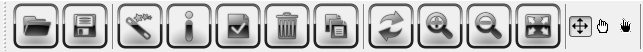
\includegraphics[scale=0.7]{images/Oct12/icon_bar.png} 
\caption{Ondex icon bar}
\label{fig:icon_bar}
\end{figure}

\begin{figure}[H]
\centering

\includegraphics[scale=0.9]{images/Oct12/icon_open_save.png} 
\caption{The ``open'' icon on the left and the ``save'' icon on the right. Also available from the File menu.}
\label{fig:icon_open_save}
\end{figure}

\begin{figure}[H]
\centering

\includegraphics[scale=0.9]{images/Oct12/icon_add_i_v.png} 
\caption{The ``Add a Concept or Relation'' on the left, the ``Information on selected Concept or Relation'' icon in the middle 
and the ``Edit selected Concept or Relation'' on the right.
Available in the menus from Edit -$>$ Concept / Relation -$>$ Add New, View -$>$ Item Info, Edit -$>$ Concept / Relation -$>$ Edit Selected.}
\label{fig:icon_add_i_v}
\end{figure}

\begin{figure}[H]
\centering
\includegraphics[scale=0.9]{images/Oct12/icon_del_clone.png} 
\caption{The ``Delete selected Concept or Relation'' icon on the left and the ``Copy whole Network as new'' icon on the right.
Available in the menus from Edit -$>$ Concept / Relation -$>$ Delete Selected and Edit -$>$ Clone Network.}
\label{fig:icon_del_clone}
\end{figure}

\begin{figure}[H]
\centering
\includegraphics[scale=0.9]{images/Oct12/icon_refresh_zoom2_center.png} 
\caption{The ``Refresh Layout'', ``Zoom In'', ``Zoom Out'' and ``Center Network'' icons from left to right.
Available in the menus from Appearance -$>$ Refresh Layout, Appearance -$>$ Zoom, Appearance -$>$ Center Network.}
\label{fig:icon_refresh_zoom2_center}
\end{figure}

\begin{figure}[H]
\centering
\includegraphics[scale=0.9]{images/Oct12/icon_mouse_modes.png} 
\caption{The left-hand side icon sets the mouse to ``transforming'' mode (to move within the network) whereas the
white hand icon sets the mouse to ``picking'' mode (to select concepts, drag and drop them).
When a graph is not dense, the two modes interchange depending on the position of the mouse (positioned over blank or over concept or relation).
When a graph is dense, manually selecting a mode can be useful.
The black hand sets the mouse to ``annotating'' mode for annotation purposes.
All available from Edit -$>$ Mouse mode.}
\label{fig:icon_mouse_modes}
\end{figure}


%%%%%%%%%%%%%%%%%%%%%%%%%%%%%%%%%%%%%%%%%%%%%%%%%%%%%%%%%%%%%%%%%%%%%%%%%%%%%%%%%%%%%%%%%%%%%%%%%%%%%%%%%%%%%%%%%%%%%%%%%%%%%%%%%%%%%%%%%%%%%%%%%%%%%%%%%%
\section{Search bar in toolbar}
\label{sec:ref_search}
Ondex includes a Search feature, which enables you to quickly find concepts by searching their names, accessions and other properties. 
The default mode of the Search feature is Keyword search, other modes like chemical similarity or UniProt identifier are also available.

\begin{figure}[H]
\centering
\includegraphics[scale=0.7]{images/Oct12/search_bar.png} 
\label{fig:search_bar}
\caption{Search bar}
\end{figure}

If you select (single click) one item in the search results, you will need to click on the icon ``Zoom In'' in order for Ondex to zoom in on this particular concept. 
You can then use the mouse scroll functionality to get to the concept.
If you select several items (using the Control key) in the search results, Ondex will automatically zoom in to show all those items as close up as possible.

\textbf{Configuring an Ondex Search }
\begin{itemize}
\item At the end of the toolbar in Keyword search mode, there are 2 options that can be configured for each search. 
If you tick ``Regular Expr.'', you may enter a JAVA regular expression. An example would be: p$\backslash$$\backslash$d\{1,4\}.
It will match a ``p'' followed by 1 to 4 digits. 
For more information on regular expressions in JAVA, please visit \url{http://docs.oracle.com/javase/tutorial/essential/regex/}.
If you tick ``Case Sensitive'', the search will be sensitive to lower/upper case of each character.
\item Under the search box, there are 3 drop-down lists which allow users to restrict their search (by Concept Class, Data Source or Tag).
\end{itemize}


%%%%%%%%%%%%%%%%%%%%%%%%%%%%%%%%%%%%%%%%%%%%%%%%%%%%%%%%%%%%%%%%%%%%%%%%%%%%%%%%%%%%%%%%%%%%%%%%%%%%%%%%%%%%%%%%%%%%%%%%%%%%%%%%%%%%%%%%%%%%%%%%%%%%%%%%%%
\section{Menu system}
\label{sec:ref_menus}
 
\subsection{File}
\label{sec:menu_file}
The File menu contains basic file functionality.
\begin{itemize}
\item New: creates a new empty network 
\item Open: opens an Ondex network from a file
\item Import Expression Data: launches a wizard to import data from a tab, space or comma delimited file into the network 
\item Save graph as: saves Ondex network in a file
\item Save image as: saves the visualisation content as an image
\item Import: imports files in certain network formats, see \ref{sec:ref_loading}
\item Export: exports network to certain formats, see \ref{sec:ref_sav}
\item Print: prints the visualisation window content
\item Exit: exits Ondex
\end{itemize}

\subsection{Edit}
\label{sec:menu_edit}
\begin{itemize}
\item Undo: to undo last change (only available on right-click actions and filters)
\item Undo All: to undo all changes (same restriction)
\item Redo: to redo last change (only available on right-click actions and filters)
\item Redo All: to redo all changes (same restriction)
\item Revert Visibility to Last Save: to go back to the way the graph was the last time it was saved
\item Labels: to change concept label font, composition (to allow for various names to be displayed next to each concept on the graph) or to change relation label font
\item Delete Hidden Items: to remove invisible items from the network
\item Concept / Relation -$>$ Add New, Edit Selected, Delete Selected
\item Mouse Mode -$>$ Transforming, Picking, Annotating (see end of Section \ref{sec:ref_icons})
\item Clone Network: to copy whole network as new (useful to do comparisons)
\item Settings: to set up notifications or auto-save of graph (as well as login information for developers only)
\end{itemize}

\subsection{View}
\label{sec:menu_view}
\begin{itemize}
\item Metagraph: to display a metagraph containing all the types of concepts/relations contained in the main network
\item Legend: to modify colours/shapes of concepts/relations
\item Item Info: to display information on selected items (concepts/relations) of the network
\item List: to display a list of all concepts or relations (also allows users to choose which labels to display)
\item Tabular Graph Editor: to edit concepts and relations using tables (rather than the graph)
\item Satellite View: to open a movable overview of the network
\item Windows: to view a list of all the windows opened in Ondex (also allows users to display, minimize, maximize or close all windows)
\end{itemize}


\subsection{Appearance} 
\label{sec:menu_app}
\begin{itemize}
\item Labels: to shows the names of concepts/relations/both on the main network
\item Layouts: a collection of algorithms to organise networks visually (described below)
\item Colour Concepts:
 \begin{itemize}
 \item by Data Source:
 colours concepts based on their data source
 \item by Concept Class:
 colours concepts based on their concept class
 \item by Evidence Type:
 colours concepts based on their evidence type
 \end{itemize}
\item Colour Relations:
 \begin{itemize}
 \item by Relation Type:
 colours relations based on their relation type
 \item by Evidence Type:
 colours relations based on their evidence type
 \end{itemize}
\item Shape Relations:
\begin{itemize}
 \item using Quad Curves
 \item using Cubic Curves
 \item using Bent Lines
 \item using Straight Lines
 \item Draw arrows (untick to remove arrows on relations)
 \end{itemize}
\item Smooth Relations: anti-aliasing painting of relations in the network
\item Show MouseOver: enable mouse over display of chemical drawings on nodes
\item Update Display: to update the visualisation window with recent modifications
\item Load Appearance: to load some or all items of appearance that had been previously saved
\item Save Appearance: to save layout, concept colours, concept shapes, concept sizes, relation colours and relation widths
\item Center Network: centers the network within the visualisation window
\item Refresh Layout: to get back to the latest layout that was drawn (e.g. useful after moving concepts and relations around)
\item Zoom: zoom in or out
\end{itemize}


\subsubsection{Layouts:}
\begin{itemize}
\item Circular:
for a circular arrangement corresponding to concept classes
\item Gem:
for the Gem layout algorithm\footnote{
Frick A., Ludwig A. and Mehldau H. (1994). ``A Fast Adaptive Layout Algorithm for Undirected Graphs (Extended Abstract and System Demonstration)''. 
Lecture Notes In Computer Science; Vol. 894. Proceedings of the DIMACS International Workshop on Graph Drawing, 388--403.}:
\item More:
  \begin{itemize}
  \item Connectivity:
  for a mixture of the circular and hierarchical layouts
  \item Flip:
  for a flip around of selected concepts (mirror effect)
  \item Force Directed:
  for a force-directed algorithm based on attributes values
  \item Genomics:
  for a view of the data where chromosomes are represented as batons
  \item Hierarchical:
  for a hierarchy arranged by concept classes
  \item Kamada-Kawai:
  for the Kamada-Kawai layout algorithm\footnote{Kamada T. and Kawai S. (1989). ``An algorithm for drawing general undirected graphs.'' Information Processing Letters, 31, 7--15.}
  \item LinLog:
  for the LinLog layout algorithm\footnote{\url{http://www.informatik.tu-cottbus.de/~an/GD/linlog.html}}
  \item Radial Tree:
  for a layout determined by tree extraction and polar coordinates
  \item Relation Type Specific:
  for a force-directed algorithm based on relation types
  \item Static:
  for the latest saved layout
  \item Sugiyama:
  for the Sugiyama layout algorithm\footnote{Sugiyama, K. and Misue, K. ``Visualization of structural information: Automatic drawing of compound digraphs'', 1991.}
  \item Tree:
  for a directed rooted tree
  \end{itemize}
\item Layout Options:
for options on the parameters of some algorithms (some algorithms do not have options, others do but are not yet supported)
\end{itemize}


\subsection{Tools}
\label{sec:menu_tools}
\begin{itemize}
\item Integrator: user interface to allow users to create their own data integration pipeline (see Section \ref{sec:integrator})
\item Filters: a collection of algorithms to make some concepts/relations invisible (described below)
\item Annotators: a collection of algorithms to visualise the data held on concepts/relations (described below)
\item Selecting Concepts/Relations: this submenu allows users to select all concepts/relations on the network, or invert their original selection
\item Console: a scripting console (see Section \ref{sec:parsing_tabdel}) 
\item Popup Editor: create JavaScript based custom right click functionality 
\item Statistics: displays statistics about the opened network
\end{itemize}


\subsubsection{Filters:}
   \begin{itemize}
   \item Neighbourhood: to see a particular number of neighbours only around a particular concept 
   \item Tag: narrows down the graph to all concepts which were annotated with the same tag
   \item Unconnected: filters out all unconnected concepts
   \item More:
	\begin{itemize}
	\item Attribute Value Matcher: filters out concepts or relations based on a given attribute and value
	\item Concept Class: filters out some particular class of concepts
	\item Data Source: filters out concepts from a specified data source
	\item Defluff: filters out single-linked chains that otherwise end in unconnected concepts
	\item Degree: filters out concepts that have a number of ingoing/outgoing relations that is less than, equal or greater than the numbers set by the user in the filter window
	\item Evidence Type: filters out concepts from a specified evidence type
	\item Genomics: shows only genes of the specified regions and their neighbourhood
	\item Missing Relation Type: filters out concepts which are missing a specified type of relation
	\item Relation Type: filters out some particular type of relations
	\item Scatter Plot: filters concepts according to two attributes values selected in a scatter plot 
	\item Shortest Paths:
	  \begin{enumerate}
	  \item All Pairs Shortest Path:
	  computes the shortest paths between all possible pairs of concepts and removes all relations that are not part of these shortest paths
	  \item Shortest Path:
	  computes the Dijkstra shortest path algorithm from a particular concept 
	  \item Single Shortest Path:
	  computes the shortest path between two given concepts
	  \end{enumerate}
	\item SubGraph:
	filters out all concept classes and relation types that are not selected by the user in this sort of metagraph (from a concept selected by the user to start with)
	\item Threshold:
	selects a threshold for one of the concepts attributes' value
	\end{itemize}
   \end{itemize}

\subsubsection{Annotators:}
   \begin{itemize}
   \item Colour Concepts by General Attribute: to colour concepts based on one of their attribute's value
   \item Scale Concepts by Numerical Value: to resize concepts based on one of their attribute's value
   \item Scale/Colour Concepts by Numerial Value: to resize and colour concepts based on one of their attribute's numerical value
   \item Scale/Colour Relations by Numerial Value: to resize and colour relations based on one of their attribute's numerical value
   \item Shape Concepts by General Attribute: to shape concepts based on one of their attribute's value
   \item More:
      \begin{itemize}
      \item Betweenness / Degree Centrality:
      to resize concepts based on their degree centrality (or hub-likeness) and change their colour depending on their betweenness centrality 
      (or how influential they are) within the network
      \item Betweenness Centrality:
      to resize concepts based on how influential they are within the network\footnote{
      Brandes U. (2001). ``A faster algorithm for betweenness centrality.'' Journal of Mathematical Sociology, Vol. 25, 163-177.}
      \item Chemical Drawings:
      to display chemical drawings on nodes which hold chemical data structure
      \item Cluster Complexity:
      Identifies all maximal cliques in a graph and ranks them according to their Shannon entropy (in physics: "disorder" of a system) measure for a given attribute 
      (for example different phenotypes in a clique). Displays the ranking and allows for selection of interesting cliques.
      \item Colour Concepts with Series Data:
      Colours concepts according to a list of numerical attributes. 
      The user can iterate over this list to select the attribute mapped to concept colour. 
      For example, iterating through expression values of different time points of a micro-array experiment one after the other.
      \item Colour Relations by Concept Tag Intersection:
      to colour relations green if the two concepts they link have more than one tag in common, red otherwise
      \item Concept Degree:
      Creates attributes ("IN\_DEGREE", "OUT\_DEGREE", "BOTH\_DEGREE") on the concepts which reflect the in- and out-degrees of the node corresponding to the concept. 
      This annotator does not change the visualisation of the graph (please apply the Attribute Value Matcher filter to do so).
      \item Degree Specificity:
      Creates attributes on the concepts and/or relations which reflect a certain set of concept class connectivity.
      \item Display Series Data on Concepts:
      Draw line or bar graphs on the nodes in the network, visualising the time series data selected.
      \item Graph Algorithms:
      to select one of five algorithms (all cliques, connected components, cut
      concepts, minimum equivalent, strongly connected). 
      Results are added as attributes to the concepts.
      \item Relation Betweenness Clusterer:
      Adds an attribute (true/false) to a chosen number of relations that have the highest betweenness measure. 
      This annotator does not change the visualisation of the graph (please apply a filter to do so). 
      After applying a filter (e.g. the Attribute Value Matcher filter), the graph would show highly connected components.
      \item Scale Concepts/Relations by Type:
      to choose the size of concepts/relations for each concept class and relation type
      \item Virtual Knock-Out:
      to remove one concept at a time virtually and calculating the structure changes in the network
      \item Weighting Relation Attribute:
      to add an attribute to relations which corresponds to a weighted calculation of the existing attributes (only works on networks where all relations have attributes)
      \end{itemize}
   \end{itemize}

\subsection{Help}
\label{sec:menu_help}
\begin{itemize}
\item About: a brief message about the project
\item Documentation: a documentation of Ondex functions with screenshots
\item Report a problem: Error reporting dialog to submit additional information
\item Tutorial: this tutorial is available in PDF format through this menu
\item Version: Current program version and system information
\item Welcome message: the welcome message which shows when starting Ondex
\end{itemize}



%%%%%%%%%%%%%%%%%%%%%%%%%%%%%%%%%%%%%%%%%%%%%%%%%%%%%%%%%%%%%%%%%%%%%%%%%%%%%%%%%%%%%%%%%%%%%%%%%%%%%%%%%%%%%%%%%%%%%%%%%%%%%%%%%%%%%%%%%%%%%%%%%%%%%%%%%%
\newpage
\section{Integrator}
\label{sec:ref_integrator}
The Ondex Integrator is Ondex's workflow manager. It is available from the Tools menu and looks like this
\begin{figure}[H]
\centering
\includegraphics[scale=0.55]{images/Oct12/integrator.png} 
\caption{Integrator}
\label{fig:integrator}
\end{figure}
There 3 main areas to the Ondex Integrator (which are all adjustable using the mouse):
\begin{itemize}
\item Top left: listing panel.
This window lists all the plugins available to add to your workflow.
\item Bottom left: documentation panel.
This window contains 4 tabs and shows documentation for the selected item (single click) in the listing panel above.
\item Right: workflow panel.
Selected plugins (double click) will appear in this window for you to set parameters.
\end{itemize}

Other useful points:
\begin{itemize}
\item File -$>$ Validate allows users to check their workflow before running it.
\item Configure -$>$ ``Show stable plugins only'' can be ticked/unticked to hide/show experimental plugins as well.
\item There is a ``Run workflow'' button at the bottom-right corner. Saving your workflow before running is advised (File -$>$ Save As).
Running the workflow will highlight the name of the plugins in yellow (while running), green (when finished).
A error report pops up when error(s) are found. A ``$>>$'' icon is placed next to each error to show users where each of them is in the pipeline.
The name of the workflow becomes
\begin{itemize}
\item orange while it is running
\item red if running has failed 
\item back to black if it completed successfully
\end{itemize}
\end{itemize}

%Information on the plugins themselves can be found on \url{http://ondex.rothamsted.ac.uk/ondex-plugins/list}.


%%%%%%%%%%%%%%%%%%%%%%%%%%%%%%%%%%%%%%%%%%%%%%%%%%%%%%%%%%%%%%%%%%%%%%%%%%%%%%%%%%%%%%%%%%%%%%%%%%%%%%%%%%%%%%%%%%%%%%%%%%%%%%%%%%%%%%%%%%%%%%%%%%%%%%%%%%
\section{Console}
\label{sec:ref_console}
The console is Ondex's scripting interface. It is available from the Tools menu and looks like this
\begin{figure}[H]
\centering
\includegraphics[scale=0.7]{images/Oct12/console.png} 
\caption{Console}
\label{fig:console}
\end{figure}
Section \ref{sec:parsing_tabdel} explains how to import tab-delimited data files using it.

%%%%%%%%%%%%%%%%%%%%%%%%%%%%%%%%%%%%%%%%%%%%%%%%%%%%%%%%%%%%%%%%%%%%%%%%%%%%%%%%%%%%%%%%%%%%%%%%%%%%%%%%%%%%%%%%%%%%%%%%%%%%%%%%%%%%%%%%%%%%%%%%%%%%%%%%%%
\section{Statistics}
\label{sec:ref_stats}
The statistics module is available from the Tools menu.
You see a window that is divided into 3 main areas as shown in Figure \ref{fig:stats}.
\begin{itemize}
\item Top left: listing panel.
It contains 4 lists with different graph elements that can be used as variables or filters.
\item Top right: selection panel.
It contains the variable field (with two buttons that load it with the currently selected element or unload it, respectively).
The filters list is below the variable field (same buttons to load/unload).
Select from the listing panel and enter in value(s) of your choice.
They will be handled as conditions linked with an ``or'' operation.
\item Bottom: display panel.
It shows the number of concepts that were found that meet the selected conditions and the respective number of relations.
In case the variable is a numerical value, it also features the mean and the standard deviation values, and a histogram.
\end{itemize}

\begin{figure}[H]
\centering
\includegraphics[scale=0.6]{images/Oct12/stats.png} 
\caption{Statitics module}
\label{fig:stats}
\end{figure}

 % 3 Reference

%%%%%%%%%%%%%%%%%%%%%%%%%%%%%%%%%%%%%%%%%%%%%%%%%%%%%%%%%%%%%%%%%%%%%%%%%%%%%%%%%%%%%%%%%%%%%%%%%%%%%%%%%%%%%%%%%%%%%%%%%%%%%%%%%%%%%%%%%%%%%%%%%%%%%%%%%%%%%%%%%%%%
\chapter{How do I compare genomic data in Ondex?}
\label{cha:comp}
%%%%%%%%%%%%%%%%%%%%%%%%%%%%%%%%%%%%%%%%%%%%%%%%%%%%%%%%%%%%%%%%%%%%%%%%%%%%%%%%%%


\section*{Application case: Combining comparative genomics with data integration for the prediction of potential pathogenicity genes}
\label{sec:phi_bot_app}
We integrated PHI-base (\url{http://www.phi-base.org/}), a database containing expertly curated molecular and biological information on genes 
proven to affect the outcome of pathogen-host interactions. 
Additionally, we loaded the genome sequence of \textit{Botrytis cinerea} (\url{http://www.broad.mit.edu/annotation/genome/botrytis_cinerea/}).
See section \ref{sec:integrator} for more information.

Running our implementation of the InParanoid algorithm\footnote{Remm M., Storm C.E., Sonnhammer E.L. (2001). 
``Automatic clustering of orthologs and in-paralogs from pairwise species comparisons''. Journal of Molecular Biology, 314(5):1041-52, PubMed ID: 11743721.}
based on BLAST mappings of the genomic data gives us new biological insights. 
Indeed PHI-base contains a lot of annotation which can be displayed on the network using the ``Annotators'' menu. 
This type of visualization in Ondex allows us to gain new hypotheses on the \textit{Botrytis} genome.

After loading the data file botrytis\_phibase.oxl from the directory Tutorial\_files/Application\_cases, a metagraph is displayed. 
The metagraph (see Figure \ref{fig:bot_metagraph}) shows red circles are proteins from \textit{Botrytis} and blue triangles are proteins from PHI-base 
(see explanation for ``Interaction:Protein'' in section \ref{sec:integrator}).

\begin{figure}[H]
\centering
\includegraphics[scale=0.35]{images/Oct12/app2fig1.png} 
\caption{Circular layout, metagraph and item information window}
\label{fig:bot_metagraph}
\end{figure}

They are linked by orthologue and paralogue relations indicating whether genes were separated by the event of speciation (ortholog) or 
genetic duplication (paralog). 
Orthologs retain the same function in the course of evolution, whereas paralogs evolve new functions, even if these are related to the original one. 
Concepts imported from PHI-base contain a lot of annotation. 
In order to make this annotation visible, we are going to use the ``Annotators'' menu. 
First of all, let us use the ``Colour Concepts by General Attribute'' annotator (see Figure \ref{fig:bot_colbyval}).

\begin{figure}[H]
\centering
\includegraphics[scale=0.35]{images/Oct12/app2fig2.png} 
\caption{Colour Concepts by General Attribute annotator}
\label{fig:bot_colbyval}
\end{figure}

As a lot of phenotypic information is encoded in PHI-base, we select the first attribute: ``Phenotype''. 
Then click on ``Annotate Graph''. 
We get a colour legend and colour annotation on the triangles (PHI-base concepts) 
in the graph as shown in Figure \ref{fig:bot_colbyval_res}.

\begin{figure}[H]
\centering
\includegraphics[scale=0.35]{images/Oct12/app2fig3.png} 
\caption{Results of the Colour Concepts by General Attribute annotator}
\label{fig:bot_colbyval_res}
\end{figure}

We use Appearance $->$ Layouts $->$ Gem in order to visualize clusters (see Figure \ref{fig:bot_gem}).

\begin{figure}[H]
\centering
\includegraphics[scale=0.35]{images/Oct12/app2fig4.png} 
\caption{After applying the Gem layout}
\label{fig:bot_gem}
\end{figure}

We may now zoom in on a particular cluster as shown in Figure \ref{fig:bot_zoom_in}.

\begin{figure}[H]
\centering
\includegraphics[scale=0.35]{images/Oct12/app2fig5.png} 
\caption{Zooming in on a cluster}
\label{fig:bot_zoom_in}
\end{figure}

Another Annotator we may use is the ``Shape Concepts by General Attribute'' annotator as PHI-base also contains information about the pathogen species. 
We select the attribute ``Taxonomy\_ID'' (NCBI Taxonomy Identifier) in the list as shown in Figure \ref{fig:bot_taxid}.

\begin{figure}[H]
\centering
\includegraphics[scale=0.35]{images/Oct12/app2fig6.png} 
\caption{Selecting an attribute}
\label{fig:bot_taxid}
\end{figure}

We can look up the concepts' Taxonomy identifier in their corresponding Item Information as shown in Figure \ref{fig:bot_taxid_lookup1}.

\begin{figure}[H]
\centering
\includegraphics[scale=0.35]{images/Oct12/app2fig7.png} 
\caption{Taxonomy identifier in Item Information}
\label{fig:bot_taxid_lookup1}
\end{figure}

Once you know what Taxonomy identifier a concept holds, you may enter it in the box below and choose a shape you would like to associate to it (see Figure \ref{fig:bot_shape_before}).

\begin{figure}[H]
\centering
\includegraphics[scale=0.35]{images/Oct12/app2fig8.png} 
\caption{Applying the Shape Concepts by General Attribute annotator}
\label{fig:bot_shape_before}
\end{figure}

The results after clicking on ``Annotate Graph'' are shown on Figure \ref{fig:bot_shape_after}.

\begin{figure}[H]
\centering
\includegraphics[scale=0.35]{images/Oct12/app2fig9.png} 
\caption{After applying the Shape Concepts by General Attribute annotator}
\label{fig:bot_shape_after}
\end{figure}

Let us change the shapes of all the PHI-base concepts in this cluster by using the same annotator several times (see Figures \ref{fig:bot_shape21} and \ref{fig:bot_shape22}). 
(Note: Entering more than one Taxonomy identifier in the blank box would make the same shape be associated to all of those Taxonomy identifiers.)

\begin{figure}[H]
\centering
\includegraphics[scale=0.35]{images/Oct12/app2fig10.png} 
\caption{Applying the Shape Concepts by General Attribute annotator again}
\label{fig:bot_shape21}
\end{figure}

\begin{figure}[H]
\centering
\includegraphics[scale=0.35]{images/Oct12/app2fig11.png} 
\caption{After applying the Shape Concepts by General Attribute annotator a third time}
\label{fig:bot_shape22}
\end{figure}
In this example we have shown how data integration combined with visualisation of annotations from a manually curated database 
can be used for guild-by-association studies to yield hypotheses for a newly sequenced genome.


\newpage
 % 4 How do I compare genomic data in Ondex?

%%%%%%%%%%%%%%%%%%%%%%%%%%%%%%%%%%%%%%%%%%%%%%%%%%%%%%%%%%%%%%%%%%%%%%%%%%%%%%%%%%%%%%%%%%%%%%%%%%%%%%%%%%%%%%%%%%%%%%%%%%%%%%%%%%%%%%%%%%%%%%%%%%%%%%%%%%%%%%%%%%%%
\chapter{How do I analyse micro-array data using Ondex?}
\label{cha:pie}
%%%%%%%%%%%%%%%%%%%%%%%%%%%%%%%%%%%%%%%%%%%%%%%%%%%%%%%%%%%%%%%%%%%%%%%%%%%%%%%%%%


\section*{Application case: Analysing Experimental Data in the context of Integrated Biological Networks}
\label{sec:pie_charts_app}

We integrated AraCyc (\url{http://www.arabidopsis.org/biocyc/index.jsp}), a database containing pathway information for the plant 
\textit{Arabidopsis thaliana}, with data from the former DRASTIC-INSIGHT database for information on plant gene expression. 
Additionally, we loaded micro-array expression data onto the concepts of the network using attributes. 
(A workflow named pathways\_expdata\_integrator\_workflow.xml is available under Tutorial\_files/Application\_cases for this data integration pipeline).
The expression data has been analysed for statistical significance and normalized.
We show that an integrative approach to the exploration of micro-array expression data can leverage the understanding in the context of pathways 
and might yield new biological insights.
\begin{figure}[H]
\centering
\includegraphics[scale=0.35]{images/Oct12/app1fig1.png} 
\caption{Metagraph}
\label{fig:metagraph_pathways}
\end{figure}
After loading the data file Tutorial\_files/Application\_cases/pathways\_expdata.oxl, a metagraph is displayed in Figure \ref{fig:metagraph_pathways}.
The different concept classes are:
\begin{itemize}
\item Genes from the DRASTIC database, which did not map to any AraCyc genes
\item Treatments (e.g. drought, ABA) from the DRASTIC database under which a gene showed a significant change in expression
\item Merged entities consisting of Genes from DRASTIC and Proteins from AraCyc together with microarray expression data to achieve a more compact pathway representation
\item Protein complexes described in AraCyc
\item Proteins in AraCyc, for which there is no expression data available
\item Enzymes catalysing reactions from AraCyc
\item Enzyme classifications for enzymes from AraCyc
\item Chemical compounds involved with reactions and enzymes in AraCyc
\item Reactions belonging to an AraCyc pathway
\item AraCyc pathways which can be part of a hierarchy
\item Publications assigned to entries in AraCyc
\end{itemize}

\begin{figure}[H]
\centering
\subfigure[Metadata - Concept Classes tab]{
\includegraphics[scale=0.5]{images/Oct12/app1fig2_1.png} 
\label{fig:CCs}
}
\subfigure[Metadata - Relation Types tab]{
\includegraphics[scale=0.5]{images/Oct12/app1fig2_2.png} 
\label{fig:RTs}
}
\label{fig:metadata_pathways}
\caption{Metadata - legend and numbers}
\end{figure}
The whole network contains 24541 concepts and 45153 relations as shown in Figure \ref{fig:metadata_pathways}. 
Using tag information we can display only the relevant sub-network instead of having to work with the whole network.

\begin{figure}[H]
\centering
\includegraphics[scale=0.35]{images/Oct12/app1fig3.png} 
\caption{Tag filter}
\label{fig:tag_filter}
\end{figure}

From the tag drop-down list please select gamma-glutamyl-cycle as shown in Figure \ref{fig:tag_filter}.
The resulting graph is shown in Figure \ref{fig:tag_result}.

\begin{figure}[H]
\centering
\includegraphics[scale=0.35]{images/Oct12/app1fig4.png} 
\caption{Tag filter results}
\label{fig:tag_result}
\end{figure}

The Gem layout (Appearance $->$ Layouts $->$ Gem) can easily be applied to this smaller network, which produces a more pleasant representation of the network
(see Figure \ref{fig:tag_gem}).

\begin{figure}[H]
\centering
\includegraphics[scale=0.35]{images/Oct12/app1fig5.png} 
\caption{After applying the Gem layout}
\label{fig:tag_gem}
\end{figure}

Now additional features like displaying concept and relation labels (Appearance $->$ Labels) 
and anti-aliased painting (Appearance $->$ Smooth Relations) can be turned on to enrich the current visualisation. 
Using the Mouse wheel you can zoom into the network view. Try to locate a group of ``membrane alanyl aminopeptidases'' (see Figure \ref{fig:membrane}).

\begin{figure}[H]
\centering
\includegraphics[scale=0.35]{images/Oct12/app1fig6.png} 
\caption{After zooming in}
\label{fig:membrane}
\end{figure}

Here only one Gene (blue circle) has information associated from the DRASTIC databases (purple circle). 
On all of these three genes additional information can be displayed by right-clicking on a concept (see Figure \ref{fig:properties}).

\begin{figure}[H]
\centering
\includegraphics[scale=0.35]{images/Oct12/app1fig7.png} 
\caption{Concept properties}
\label{fig:properties}
\end{figure}

By clicking on ``Show / Edit Properties'' you are able to inspect all the properties assigned to this concept. 
Selecting ``View/Edit Concept Attributes'' displays a tab based representation of all values of the attributes (see Figure \ref{fig:gds}).

\begin{figure}[H]
\centering
\includegraphics[scale=0.35]{images/Oct12/app1fig8.png} 
\caption{Concept attributes}
\label{fig:gds}
\end{figure}

In this case the values of the attributes are the microarray expression data listed according to the treatment. 
Now we can use the ``Scale Concepts by Numerical Value'' annotator (Tools $->$ Annotators $->$ Scale Concepts by Numerical Value) 
to actually map the values of the attributes to the visualisation of the corresponding concepts (see Figure \ref{fig:scale}).

\begin{figure}[H]
\centering
\includegraphics[scale=0.35]{images/Oct12/app1fig9.png} 
\caption{Scale Concept by Numerical Value annotator}
\label{fig:scale}
\end{figure}

The annotator supports multiple value selection. 
Here all treatments of the form 0NxC are selected. 
Annotate Graph performs the changes to the visualisation.
Figure \ref{fig:scale_results} shows the results.

\begin{figure}[H]
\centering
\includegraphics[scale=0.35]{images/Oct12/app1fig10.png} 
\caption{Results of the Scale Concept by Numerical Value annotator}
\label{fig:scale_results}
\end{figure}

The visualisation for the concepts now changed to pie charts. 
The pie chart is divided into the number of treatments that were selected in the annotator. 
It displays information from the top clockwise in the order in which they appear in the annotator
(it is possible to drap and drop the order around in the annotator). 
Visual inspection of this network now reveals that the gene at the top shows a constant expression pattern, 
whereas the other two Genes are differently regulated (red for up-regulation and green for down-regulation).

\begin{figure}[H]
\centering
\includegraphics[scale=0.35]{images/Oct12/app1fig11.png} 
\caption{Further analysis}
\label{fig:further}
\end{figure}

Further inspection (see Figure \ref{fig:further}) of the attribute's value of the bottom gene supports the hypothesis 
that the up measurement might be wrong and the Gene might have been down-regulated across all three conditions. 
In addition we can annotate this gene with information from the DRASTIC database showing that 
this particular gene has a significant change in expression under the associated conditions. 

It is also possible to have a second visualisation window showing the same graph with different annotations.
To do so, use the 7th icon (``Copy whole Network as new'') or use the Edit menu -$>$ Clone Network.
A question will pop up ``Do you want to link views?''. 
If you answer no, the whole graph will load up using the circular layout.
If you answer yes, the concepts/relations visible in your current visualisation window will appear in the second one (at the same positions),
as shown in Figure \ref{fig:copygraph}.

\begin{figure}[H]
\centering
\includegraphics[scale=0.35]{images/Oct12/app1fig12.png} 
\caption{Copy whole graph}
\label{fig:copygraph}
\end{figure}

Figure \ref{fig:clone} shows how moving concepts happen in both windows from then on
and that different annotations can be displayed.

\begin{figure}[H]
\centering
\includegraphics[scale=0.35]{images/Oct12/app1fig13.png} 
\caption{Layout is linked across both windows}
\label{fig:clone}
\end{figure}

{\em{Summary}}\\
In this example, we showed how visualisation of expression patterns can leverage the understanding 
in terms of comparing conditions and influence on pathways. We identified one particular Gene with an irregular expression pattern. 
Furthermore, data integration helped to enrich pathways from AraCyc with information about influential treatments from DRASTIC.  % 5 How do I analyse micro-array data using Ondex?

%%%%%%%%%%%%%%%%%%%%%%%%%%%%%%%%%%%%%%%%%%%%%%%%%%%%%%%%%%%%%%%%%%%%%%%%%%%%%%%%%%%%%%%%%%%%%%%%%%%%%%%%%%%%%%%%%%%%%%%%%%%%%%%%%%%%%%%%%%%%%%%%%%%%%%%%%%%%%%%%%%%%
\chapter{How do I look at QTLs in Ondex?}
\label{cha:qtl}
%%%%%%%%%%%%%%%%%%%%%%%%%%%%%%%%%%%%%%%%%%%%%%%%%%%%%%%%%%%%%%%%%%%%%%%%%%%%%%%%%%
%Intro TO DO

\section*{Application case: Candidate genes for biomass traits}
\label{sec:k1}

As there is a need to understand plant architecture related to yield ({\it{e.g.}}, branching process),
we wish to identify genes controlling biomass production in willow (a second generation bioenergy crop). 
Even well-defined QTL may encompass many potential candidate genes (perhaps hundreds),
it is therefore difficult to objectively choose underlying candidate(s) that drive the phenotype.
We are developing means to support systematic analysis of QTL regions and to prioritise genes for experimental analyses.

The willow genome is not yet fully sequenced.
Poplar is the first tree with a fully sequenced genome.
It has 19 chromosomes, 45555 predicted genes (4 times larger than \textit{Arabidopsis's} genome).
Not much is known yet about the function of poplar genes.

We are using comparative genomics to compare poplar to \textit{Arabidopsis} to find linked references, expression patterns, pathways, plant hormones and ontologies
in order to link genes between the two.
The genome annotation pipeline integrates data together from UniProtKB, TAIR, Gramene, GO, GOA, TraitOnt, PlantOnt, Medline, AraCyc and Pfam.
(A workflow named biomass\_integrator\_workflow.xml is available under Tutorial\_files/Application\_cases for this data integration pipeline).
The methods used for this integration are based on sequence similarity, domain analysis and text mining as shown in Figure \ref{fig:poplar_annotation_pipeline}.
This allows us to achieve automatic function prediction with different levels of evidence.

\begin{figure}[H]
\centering
\includegraphics[scale=0.8]{images/Oct12/poplarkb_pipeline.png} 
\caption{Poplar annotation pipeline}
\label{fig:poplar_annotation_pipeline}
\end{figure}

This data integration in Ondex resulted in the metagraph shown in Figure \ref{fig:poplar_metagraph}.
(The data is available under Tutorial\_files/Application\_cases, the graph is named biomass\_knowledge\_base\_subset.oxl).
Inspection of the metagraph shows the genes and the QTLs enriched with positional information as well as
the proteins annotated with GO, EC, KEGG and publications based on comparative genomics and protein family analysis.
\begin{figure}[H]
\centering
\includegraphics[scale=0.35]{images/Oct12/poplarkb_metagraph.png} 
\caption{Integrated poplar knowledge base subset}
\label{fig:poplar_metagraph}
\end{figure}

Had we opened the entire knowledge base, the Genomics layout would have enabled us to display chromosomes, genes and QTLs 
where chromosomal regions and QTLs can be selected (see Figure \ref{fig:poplar_genomic_view}).
\begin{figure}[H]
\centering
\includegraphics[scale=0.3]{images/Oct12/poplar_genomic_view.png} 
\caption{Genomics layout (Appearance menu) or Genomics filter (Tools -$>$ Filters -$>$ More -$>$ Genomics -$>$ Switch to genomic view)}
\label{fig:poplar_genomic_view}
\end{figure}

In many domains, we observe various phenotypes without being able to link them to genes which are responsible for them.
The aim of this application case is to identify genes controlling biomass production in willow (a second generation bioenergy crop). 
We are developing software which can support biologists and users to analyse QTLs
(genomic regions that help us narrow down potential candidate genes related to a phenotype).

We currently have two sources of data:
\begin{itemize}
\item QTL data is available for willow, however the willow genome is not yet fully sequenced
\item The poplar genome sequence is available and this species is very similar to willow, however very little is known about the function of poplar genes
\end{itemize}
A QTL can contain up to hundreds of genes. We therefore look to identify candidate genes that correspond to the observed phenotype.

In order to find similar sequences in other species that hold information on gene function,
we have undertaken a comparative genomics approach.
This allows us to gather data from free text (where information then needs to be automatically extracted), 
expression patterns, pathways, ontologies, {\it{etc.}}.

The genomic view in Ondex allows users to visualise chromosomes, genes and QTLs (in red).
The genomic filter allows users to select the regions they wish to study in more detail.
Users may also enter a few keywords in a search box.
Once they click on the search button, users are presented with the genes contained in the selected QTLs of interest (blue rectangles) and
these are linked to their corresponding proteins which, in turn, are linked to the orthologs found by the comparative analysis.
The orthologs are themselves linked to the information imported during the data integration.
The keywords previously entered in the search box are then used to highlight some concepts in the graph which contain them in their properties.
This feature is very useful as it allows users to directly focus on proteins that are relevant to their research work.
On the right-hand side of the visualisation window we can see some poplar proteins which are not linked to any extra information
because no orthologs were found.

Users can zoom into particular areas of the graph, they can also select a ``hot'' candidate and look at its neighbourhood
(using the neighbourhood filter).

Here are examples of combinations of steps that can be used to analyse the data where our trait of interest is ``shoot branching'' 
or the number of axillary branches:
\begin{itemize}
\item Load Tutorial\_files/Application\_cases/biomass\_knowledge\_base\_subset.oxl
\item Launch the Genomics filter (Tools -$>$ Filters -$>$ More -$>$ Genomics)
\item Select QTL ``No. axillary branches'' on the first line (chromosome 1).
Start and end of the QTL get filled in automatically this way. Untick the second line offered. 
\item Enter ``auxin'' in search options
\item Click on ``Search Region'' (see results in Figure \ref{fig:poplarkb_search_region})
\item Now select chromosome 4 as well with the same QTL
\item Click on ``Search Region'' (see results in Figure \ref{fig:poplarkb_search_region_2})
\item Click ``Show/Hide unrelated genes'' to make visible/invisible genes that are not linked to any keyword related concepts
\item After applying the Gem layout and adding labels, we get Figure \ref{fig:poplarkb_hide_unrelated_genes}
\end{itemize}

\begin{figure}[H]
\centering
\includegraphics[scale=0.35]{images/Oct12/poplarkb_search_region.png} 
\caption{Search Region function in the Genomics Filter}
\label{fig:poplarkb_search_region}
\end{figure}

\begin{figure}[H]
\centering
\includegraphics[scale=0.35]{images/Oct12/poplarkb_search_region_2.png} 
\caption{Search Region function in the Genomics Filter with both chromosomes selected}
\label{fig:poplarkb_search_region_2}
\end{figure}


\begin{figure}[H]
\centering
\includegraphics[scale=0.35]{images/Oct12/poplarkb_hide_unrelated_genes.png} 
\caption{Show/Hide unrelated genes function in the Genomics Filter}
\label{fig:poplarkb_hide_unrelated_genes}
\end{figure}

Each QTL has a gene which encodes an enzyme that is involved in an auxin related pathway.
Pathway view can connect genes of different QTL and explain phylogenetic traits.
 % 6 How do I look at QTLs in Ondex?
%%%%%%%%%%%%%%%%%%%%%%%%%%%%%%%%%%%%%%%%%%%%%%%%%%%%%%%%%%%%%%%%%%%%%%%%%%%%%%%%%%%%%%%%%%%%%%%%%%%%%%%%%%%%%%%%%%%%%%%%%%%%%%%%%%%%%%%%%%%%%%%%%%%%%%%%%%%%%%%%%%%%
\chapter{How do I study protein-protein interactions in Ondex?}
\label{cha:ppi}
%%%%%%%%%%%%%%%%%%%%%%%%%%%%%%%%%%%%%%%%%%%%%%%%%%%%%%%%%%%%%%%%%%%%%%%%%%%%%%%%%%


\section*{Application case: Exploring interactions in \textit{Arabidopsis}}
\label{sec:artem}
Three protein-protein interaction (PPI) networks were merged in this application case.
\begin{itemize}
\item 4625 PPI from IntAct (data derived from literature curation or direct user submissions)
\item 1143 PPI from TAIR (The Arabidopsis Information Resource which contains
genome sequence, gene structure, gene product information, metabolism, gene expression, DNA and seed stocks, 
genome maps, genetic and physical markers, publications)
\item 1223 PPI from BioGrid (General Repository for Interaction Datasets which contains
collections of protein and genetic interactions from major model organism species derived from high-throughput studies and conventional focused studies
\end{itemize}

These three databases were mapped using TAIR accessions after which 3 sources of evidence were added 
in order to facilitate the identification of functionally related groups of proteins. 
They were based on:
\begin{itemize}
\item co-expression
\item sequence similarity
\item co-occurrence in scientific literature
\end{itemize}

The co-expression evidence came from ATTED II (\textit{Arabidopsis thaliana} trans-factor and cis-element prediction database),
publicly available micro-array data collected by AtGenExpress (multi-national effort to uncover \textit{Arabidopsis} transcriptome).
The database:
\begin{itemize}
\item provides co-regulated gene relationships in \textit{Arabidopsis} to estimate gene functions
\item gives the Pearson correlation coefficients of co-expressed genes in \textit{Arabidopsis} calculated from available micro-array data
\end{itemize}
The data from ATTED II is mapped using TAIR accessions again.

The sequence similarity evidence was obtained by running NCBI PSI-BLAST in order to identify similarities between our reference set of proteins
(and against the \textit{Arabidopsis} subset of UniProt).
The co-occurrence of protein names was gathered by using the integrated Apache Lucene based mapping method on 25,900 Medline abstracts related to \textit{Arabidopsis thaliana}.
At this stage, concepts in the network are connected if there is evidence from interaction, co-expression, sequence similarity or co-occurrence.
Extra information was added as attributes to concepts and relations on: 
\begin{itemize}
\item Network statistics
	\begin{itemize}
	\item Betweenness centrality (how influential a concept is) [BWC]
	\item Degree centrality (hub likeness) [DC]
	\end{itemize}
\item Markov Clustering (identifies strongly connected groups of proteins in the network)
\end{itemize}

Load Tutorial\_files -$>$ Application\_cases -$>$ ppi\_aba\_cluster.oxl in Ondex 
(this is a single cluster of the whole file available as ppi\_full\_network.oxl).
The ``Scale/Colour Relations by Numerical Value'' annotator offers users the possibility to use the rainbow scale (see online help by pressing F1)
which means the minimum values are represented in purple while the maximum ones are in red.
Figure \ref{fig:aba_cluster} shows the sources of evidence associated with the relations where the strength of the relations 
is indicated by this colour coding.
\begin{figure}[H]
\centering
\includegraphics[scale=0.5]{images/Oct12/aba_cluster.png} 
\caption{Four sources of evidence on relations (+ all of them combined) using the rainbow scale colouring}
\label{fig:aba_cluster}
\end{figure}

Here are examples of combinations of steps, annotators and filters that can be used to analyse the data:
\begin{itemize}
\item Appearance -$>$ Layouts -$>$ Gem
\item Appearance -$>$ Smooth Relations to use anti-aliased painting (see Figure \ref{fig:aba_cluster_no_ann})

\begin{figure}[H]
\centering
\includegraphics[scale=0.35]{images/Oct12/aba_cluster_no_ann.png} 
\caption{Abscisic acid cluster before annotation}
\label{fig:aba_cluster_no_ann}
\end{figure}

\item Tools -$>$ Annotators -$>$ Scale/Colour Relations by Numerical Value
\item Enter relation size of min 4 and max 4
\item Tick ``Colour relations'', ``No attribute colour'' and change colour to grey
\item Tick ``Colour on rainbow scale''
\item Select ``INTERACTION\_WEIGHT'' in list of attributes
\item Click on ``Annotate Graph'' (see results in Figure \ref{fig:aba_ann_rel})

\begin{figure}[H]
\centering
\includegraphics[scale=0.35]{images/Oct12/aba_ann_rel.png} 
\caption{Abscisic acid cluster after annotating relations}
\label{fig:aba_ann_rel}
\end{figure}

\item Tools -$>$ Annotators -$>$ Scale/Colour Concepts by Numerical Value
\item Enter concept size of min 10 and max 100
\item Tick ``No attribute size'' and enter 5
\item Tick ``Colour concepts''
\item Tick ``No attribute colour'' and select to grey
\item Tick ``Colour on rainbow scale''
\item Select ``COMBINED\_DC'' and click on ``Annotate Graph'' (see results in Figure \ref{fig:aba_ann_con})

\begin{figure}[H]
\centering
\includegraphics[scale=0.35]{images/Oct12/aba_ann_con.png} 
\caption{Abscisic acid cluster after annotating concepts}
\label{fig:aba_ann_con}
\end{figure}

\item Tools -$>$ Filters -$>$ More -$>$ Theshold	
\item Go to the ``Attributes on Relations'' tab
\item Select the ``INTERACTION\_EBWC'' (edge betweenness centrality) as attribute, a distribution should appear below (see Figure \ref{fig:aba_filter_thr1})

\begin{figure}[H]
\centering
\includegraphics[scale=0.35]{images/Oct12/aba_filter_thr1.png} 
\caption{Before applying the Threshold filter}
\label{fig:aba_filter_thr1}
\end{figure}

\item Left-click to draw a rectangle to zoom in on the tail part of the distribution
\item Click anywhere in the distribution to select a threshold
\item Click on ``Filter Graph'' (see results in Figure \ref{fig:aba_filter_thr2}, some concepts/relations should disappear)

\begin{figure}[H]
\centering
\includegraphics[scale=0.35]{images/Oct12/aba_filter_thr2.png} 
\caption{After zooming in on the distribution and applying the Threshold filter}
\label{fig:aba_filter_thr2}
\end{figure}

\item Appearance -$>$ Labels -$>$ Concepts
\item Zoom in and move concepts to look at the resulting PPI network (use shift and left-click to select a group of concepts to move)

\begin{figure}[H]
\centering
\includegraphics[scale=0.35]{images/Oct12/aba_cluster_annotated.png} 
\caption{After moving concepts to better reveal PPI}
\label{fig:aba_cluster_annotated}
\end{figure}

\end{itemize}

Experiment with the data and Ondex's tools to explore these \textit{Arabidopsis} protein-protein interactions further.
 % 7 How do I study protein-protein interactions in Ondex?

%%%%%%%%
%% Any appendices should go here. The appendix files should look just like the
%% chapter files.
%%%%%%%%
\appendix
\chapter{FAQs}
\label{cha:faqs}
%%%%%%%%%%%%%%%%%%%%%%%%%%%%%%%%%%%%%%%%%%%%%%%%%%%%%%%%%%%%%%%%%%%%%%%%%%%%%%%%%%

\begin{itemize}
\item How do I install Ondex?
See Section \ref{sec:ref_install}.

\item How do I know what a toolbar icon does?\\
Place your mouse over it and a tooltip will pop up. Alternatively, read Section \ref{sec:ref_icons}.

\item How do I know what an item of the menu does?\\
Place your mouse over the corresponding question mark and a tooltip will pop up. 
Click on the question mark to open the Ondex documentation (also available by pressing F1) which contains examples along with screenshots.

\item Can I search for a specific element in the network and get Ondex to zoom on it?\\
Yes, see Section \ref{sec:search}.

\item Is there an import wizard for tab-delimited data files?\\
Yes. When there is not a parser available to upload data into Ondex, this general tab-delimited parser can help. 
You will need to tell Ondex which column corresponds to what kind of data. 
The simplest way to use it at the moment is through the scripting interface offered in the ``Console'' (Tools -$>$ Console). 
See Section \ref{sec:parsing_tabdel} for more information.

\item What is the largest graph I can load?\\
For the GUI to respond within reasonable time, you can load up to 100,000 elements (concepts + relations). 
For such large graphs, the visualisation will be empty at the beginning. 
For a responsive visualisation please make sure not to show more than 5,000 elements (concepts + relations) at any one time.

\item I keep getting a Java heap error. What can I do?\\
You can change the amount of memory you give Ondex when launching it. 
In order to do so, change the number after the Xmx option in the command line contained in the runme script (.bat for Windows, .sh for Linux)
or update the corresponding line in the ovtk2.l4j.ini file for Windows. 
Be careful not to set this number any higher than your computer's capabilities (on 32-bit Windows it is 1200M).

\item Where can I find data files?\\
If you have downloaded the tutorial zip file, you can find data files in the tutorial directory's subfolders.
Other data files are available on \url{http://www.ondex.org/doc.html}.

\item Where can I submit a bug or a feature request?\\
\url{http://ondex.rothamsted.ac.uk} and click on``Report bugs'' or ``Request new features'' (registration/login is required).

\item How can I define new concept attributes and colour concepts based on those?\\
Right-click on a concept, select ``Show / Edit Properties'', ``View/Edit Concept attributes'', ``Add a new attribute'' (at the bottom of the window),
a ``New'' tab is created. The ``Advanced Information'' is showing and the required fields (in orange) need to be filled in. At this stage, users can either:
enter a name of their choice in ``ID Symbol'' and ``java.lang.String'' in Class for a text attribute 
(``java.lang.Integer'' for a number, ``java.lang.Double'' for a double precision number).
Click on the ``Select Attribute Name'' and select an attribute name that has been used in the past. 
Note that if you have previously entered an attribute name, you will be able to select it in this list.
Enter the value for this new attribute in the editor pane provided.
To colour concepts to show the added annotation, use the ``Colour Concepts by General Attribute'' annotator (in the ``Tools'' -$>$ ``Annotators'' menu) 
selecting the new attribute.

\item How can I avoid waiting for a big graph to be visualised?\\
You can apply filters before opening the main network. 
This will make the visual graph smaller which means it will get painted quicker.
See F1 help for a documentation on filters or Section \ref{sec:analysing} for information on various ways of filtering out data before opening the main visualisation window.


%%%%%%%%%%%%%%%%%%%%%%%%%%%%%%%%%%%%%%%%%%%%%%%%%%%%%%%%%%%%%%%%%%%%%%%%%%%%%%%%%%
\end{itemize}
 % FAQs
\chapter{List of accession types}
\label{cha:accessions}
This is a list of all the accession types (data sources) currently defined in Ondex meta-data file.
\begin{itemize}

\item{3DMET}\\ Full name: 3DMET\\ Description: A three-dimensional-structure database of natural metabolites 3DMET is a database collecting three-dimensional structures of natural metabolites - 
\url{http://www.3dmet.dna.affrc.go.jp/}

\item{AC}\\ Full name: AraCyc\\ Description: AraCyc is a metabolic pathway database for Arabidopsis thaliana that contains information about both predicted and experimentally determined pathways, reactions, compounds, genes and enzymes. - 
\url{http://www.arabidopsis.org/biocyc/}

\item{AFCS}\\ Full name: AfCS\\ Description: Alliance for Cellular Signaling - 
\url{http://www.afcs.org/}

\item{AFFYMETRIX}\\ Full name: Affymetrix\\ Description: A pioneer in genetic analysis, Affymetrix introduced highly parallel genetic assays to the marketplace by commercializing the first DNA microarray in the late 1980s. - 
\url{http://www.affymetrix.com}

\item{AHD}\\ Full name: Arabidopsis Hormone Database\\ Description: Arabidopsis Hormone Database: a comprehensive genetic and phenotypic information database for plant hormone research in Arabidopsis - Peng et al., Nucleic Acids Research 2009 37(Database issue):D975-D982; doi:10.1093/nar/gkn873 

\item{ATREGNET}\\ Full name: AtRegNet\\ Description: AtRegNet is a tool used to display the regulatory networks of Arabidopsis thaliana transcription factors. - 
\url{http://arabidopsis.med.ohio-state.edu/moreNetwork.html}

\item{BIOGRID}\\ Full name: BioGRID\\ Description: General Repository for Interaction Datasets - 
\url{http://thebiogrid.org}

\item{BKL}\\ Full name: BIOBASE Knowledge Library\\ Description: With content covering disease, drugs, gene regulation, pathways, and fully annotated genomes. - 
\url{http://www.biobase-international.com/index.php?id=databasesandtools}

\item{BRENDA}\\ Full name: Enzyme Database - BRENDA\\ Description: The Comprehensive Enzyme Information System - 
\url{http://www.brenda-enzymes.org/}

\item{BROAD}\\ Full name: Broad Institute\\ Description: Broad Institute of MIT and Harvard - 
\url{http://www.broad.mit.edu}

\item{CAMJE}\\ Full name: CAMJE\\ Description: Campylobacter jejuni proteome - 
\url{http://www.expasy.ch/sprot/hamap/CAMJE.html}

\item{CAS}\\ Full name: Chemical Abstracts Service\\ Description: CAS offers the CAS REGISTRYSM - the largest collection of substance information - as well as indexed references from more than 10,000 major scientific journals and 59 patent authorities around the world. - 
\url{http://www.cas.org/}

\item{CAZY}\\ Full name: Carbohydrate-Active enZymes\\ Description: The CAZy database describes the families of structurally-related catalytic and carbohydrate-binding modules (or functional domains) of enzymes that degrade, modify, or create glycosidic bonds. - 
\url{http://www.cazy.org/}

\item{CCSD}\\ Full name: Complex Carbohydrate Structure Database\\ Description: The Complex Carbohydrate Structure Database (CCSD) and CarbBank, an IBM PC/AT (or compatible) database management system, were created to provide an information system to meet the needs of people interested in carbohydrate science. - 
\url{http://www.boc.chem.uu.nl/sugabase/carbbank.html}

\item{CGSW}\\ Full name: Catalogue of Gene Symbols for Wheat\\ Description: A Catalogue as distributed on the MacGene CD at the 10th International Wheat Genetics Symposium. - 
\url{http://wheat.pw.usda.gov/ggpages/wgc/2003/}

\item{CHEBI}\\ Full name: Chemical Entities of Biological Interest\\ Description: Chemical Entities of Biological Interest (ChEBI) is a freely available dictionary of molecular entities focused on small chemical compounds. - 
\url{http://www.ebi.ac.uk/chebi/}

\item{CHEMBL}\\ Full name: ChEMBLdb\\ Description: ChEMBL is a database of bioactive drug-like small molecules, it contains 2-D structures, calculated properties (e.g. logP, Molecular Weight, Lipinski Parameters, etc.) and abstracted bioactivities (e.g. binding constants, pharmacology and ADMET data). - 
\url{https://www.ebi.ac.uk/chembldb/}

\item{CL}\\ Full name: Cell Ontology\\ Description: The Cell Ontology is designed as a structured controlled vocabulary for cell types. - 
\url{http://www.obofoundry.org/cgi-bin/detail.cgi?id=cell}

\item{COG}\\ Full name: Clusters of Orthologous Groups of proteins\\ Description: Clusters of Orthologous Groups of proteins (COGs) were delineated by comparing protein sequences encoded in complete genomes, representing major phylogenetic lineages. Each COG consists of individual proteins or groups of paralogs from at least 3 lineages and thus corresponds to an ancient conserved domain. - 
\url{http://www.ncbi.nlm.nih.gov/COG/}

\item{CSD}\\ Full name: Complex Carbohydrate Research Center\\ Description: The Complex Carbohydrate Research Center (CCRC) was founded at the University of Georgia (UGA) in September 1985 to answer the national need for a center devoted to increasing knowledge of the structures and functions of complex carbohydrates. - 
\url{http://www.ccrc.uga.edu/}

\item{CYORF}\\ Full name: Cyanobacteria Gene Annotation Database\\ Description: CYORF is a vehicle by which the community of cyanobacteriologists collectively annotates available genomes from cyanobacteria. - 
\url{http://cyano.genome.jp/}

\item{Corpus}\\ Full name: Corpus\\ Description: Set of publications to be analysed 

\item{DATF}\\ Full name: The Database of Arabidopsis Transcription Factors\\ Description: The Database of Arabidopsis Transcription Factors (DATF) collects all arabidopsis transcription factors (totally 1922 Loci; 2290 Gene Models) and classifies them into 64 families. - 
\url{http://datf.cbi.pku.edu.cn}

\item{DOI}\\ Full name: Digital Object Identifier\\ Description: The Digital Object Identifier (DOI) System is for identifying content objects in the digital environment. - 
\url{http://www.doi.org/}

\item{DPTF}\\ Full name: The Database of Poplar Transcription Factors\\ Description: The Database of Poplar Transcription Factors (DPTF) collects all poplar transcription factors (totally 2576 TF) and classifies them into 64 families. - 
\url{http://dptf.cbi.pku.edu.cn}

\item{DRA}\\ Full name: Drastic Insight Database\\ Description: Drastic: A Database Resource for the Analysis of Signal Transduction In Cells - 
\url{http://www.drastic.org.uk}

\item{DRUGBANK}\\ Full name: DrugBank\\ Description: The DrugBank database is a unique bioinformatics and cheminformatics resource that combines detailed drug (i.e. chemical, pharmacological and pharmaceutical) data with comprehensive drug target (i.e. sequence, structure, and pathway) information. - 
\url{http://www.drugbank.ca/}

\item{EC}\\ Full name: Enzyme Nomenclature\\ Description: SwissProt Enzyme nomenclature database ENZYME is a repository of information relative to the nomenclature of enzymes. It is primarily based on the recommendations of the Nomenclature Committee of the International Union of Biochemistry and Molecular Biology (IUBMB) and it describes each type of characterized enzyme for which an EC (Enzyme Commission) number has been provided. - 
\url{http://www.expasy.ch/enzyme/}

\item{ECOCYC}\\ Full name: EcoCyc\\ Description: Database that describes the genome and the biochemical machinery of E. coli, maintained by SRI International, Menlo Park, CA. - 
\url{http://www.ecocyc.org}

\item{EMBL}\\ Full name: EMBL-EBI International Nucleotide Sequence Data\\ Description: The EMBL Nucleotide Sequence Database (also known as EMBL-Bank) constitutes Europe's primary nucleotide sequence resource. - 
\url{http://www.ebi.ac.uk/embl/}

\item{EMBLC}\\ Full name: EMBL-EBI International Nucleotide Sequence Data Clones\\ Description: The EMBL Nucleotide Sequence Database (also known as EMBL-Bank) constitutes Europe's primary nucleotide sequence resource. - 
\url{http://www.ebi.ac.uk/embl/}

\item{ENCODE}\\ Full name: ENCyclopedia Of DNA Elements\\ Description: The National Human Genome Research Institute (NHGRI) launched a public research consortium named ENCODE, the Encyclopedia Of DNA Elements, in September 2003, to carry out a project to identify all functional elements in the human genome sequence. - 
\url{http://www.genome.gov/10005107}

\item{ENSEMBL}\\ Full name: Ensembl project\\ Description: The Ensembl project produces genome databases for vertebrates and other eukaryotic species, and makes this information freely available online. - 
\url{http://www.ensembl.org}

\item{EO}\\ Full name: Environment Ontology\\ Description: A set of standardized controlled vocabularies to describe various types of treatments given to a individual plant / a population or a cultured tissue and/or cell type sample to evaluate the response on its exposure. It also includes the study types, where the terms can be used to identify the growth study facility. Each growth facility such as field study, growth chamber, green house etc is a environment on its own it may also involve instances of biotic and abiotic environments as supplemental treatments used in these studies. - 
\url{http://www.gramene.org/plant\_ontology/ontology\_browse.html}

\item{EPD}\\ Full name: Eukaryotic Promoter Database\\ Description: The Eukaryotic Promoter Database is an annotated non-redundant collection of eukaryotic POL II promoters, for which the transcription start site has been determined experimentally. - 
\url{http://www.epd.isb-sib.ch}

\item{FLYBASE}\\ Full name: FlyBase\\ Description: A Database of Drosophila Genes and Genomes - 
\url{http://flybase.org/}

\item{GENB}\\ Full name: GenBank\\ Description: GenBank Nucleic Acid Sequence Database - 
\url{http://www.ncbi.nlm.nih.gov/Genbank/}

\item{GENEDB}\\ Full name: GeneDB\\ Description: The GeneDB project is a core part of the Sanger Institute Pathogen Sequencing Unit's (PSU) activities. - 
\url{http://www.genedb.org/}

\item{GO}\\ Full name: Gene Ontology\\ Description: The Gene Ontology project is a major bioinformatics initiative with the aim of standardizing the representation of gene and gene product attributes across species and databases. - 
\url{http://www.geneontology.org/}

\item{GOAEBI}\\ Full name: Gene Ontology Annotation\\ Description: The GOA project aims to provide high-quality Gene Ontology (GO) annotations to proteins in the UniProt Knowledgebase (UniProtKB) and International Protein Index (IPI) and is a central dataset for other major multi-species databases; such as Ensembl and NCBI. - 
\url{http://www.ebi.ac.uk/GOA/}

\item{GR}\\ Full name: Gramene\\ Description: A Resource for Comparative Grass Genomics - 
\url{http://www.gramene.org/}

\item{GeneRIF}\\ Full name: Gene Reference Into Function\\ Description: GeneRIF provides a simple mechanism to allow scientists to add to the functional annotation of genes described in Entrez Gene. - 
\url{http://www.ncbi.nlm.nih.gov/projects/GeneRIF}

\item{GrainGenes}\\ Full name: GrainGenes\\ Description: A database for Triticeae and Avena - 
\url{http://wheat.pw.usda.gov/GG2/index.shtml}

\item{HGNC}\\ Full name: HUGO Gene Nomenclature Committee\\ Description: Gene Nomenclature Committee HUGO symbols - Giving unique and meaningful names to every human gene. - 
\url{http://www.genenames.org/}

\item{HINVDB}\\ Full name: H-InvDB\\ Description: H-Invitational Database (H-InvDB) is an integrated database of human genes and transcripts. - 
\url{http://hinvdb.ddbj.nig.ac.jp/ahg-db/index.jsp}

\item{HOMSTRAD}\\ Full name: HOMologous STRucture Alignment Database\\ Description: HOMSTRAD (HOMologous STRucture Alignment Database) is a curated database of structure-based alignments for homologous protein families. - 
\url{http://tardis.nibio.go.jp/homstrad}

\item{HPRD}\\ Full name: Human Protein Reference Database\\ Description: The Human Protein Reference Database represents a centralized platform to visually depict and integrate information pertaining to domain architecture, post-translational modifications, interaction networks and disease association for each protein in the human proteome. - 
\url{http://www.hprd.org/}

\item{HSSP}\\ Full name: Homology-derived Secondary Structure of Proteins\\ Description: The HSSP database is a database of homology-derived secondary structure of proteins. - 
\url{http://swift.cmbi.kun.nl/gv/hssp/}

\item{HUGE}\\ Full name: Human Unidentified Gene-Encoded\\ Description: The HUGE protein database has been created to publicize the fruits of our Human cDNA project at the Kazusa DNA Research Institute. - 
\url{http://www.kazusa.or.jp/huge/}

\item{IAH}\\ Full name: Institute for Ageing and Health\\ Description: Institute for Ageing and Health, Newcastle University - 
\url{http://www.ncl.ac.uk/iah/}

\item{IMGT}\\ Full name: ImMunoGeneTics Database\\ Description: IMGT, the international ImMunoGeneTics project, is a collection of high-quality integrated databases specialising in Immunoglobulins, T cell receptors and the Major Histocompatibility Complex (MHC) of all vertebrate species. - 
\url{http://www.ebi.ac.uk/imgt/}

\item{INPARANOID}\\ Full name: InParanoid\\ Description: Eukaryotic Ortholog Groups. - 
\url{http://inparanoid.sbc.su.se/}

\item{INTACT}\\ Full name: IntAct\\ Description: IntAct provides a freely available, open source database system and analysis tools for protein interaction data. All interactions are derived from literature curation or direct user submissions and are freely available. - 
\url{http://www.ebi.ac.uk/intact}

\item{IPI}\\ Full name: International Protein Index\\ Description: IPI provides a top level guide to the main databases that describe the proteomes of higher eukaryotic organisms. - 
\url{http://www.ebi.ac.uk/IPI}

\item{IPRO}\\ Full name: InterPro\\ Description: A database of protein families, domains and functional sites in which identifiable features found in known proteins can be applied to unknown protein sequences. - 
\url{http://www.ebi.ac.uk/interpro}

\item{IRGSP}\\ Full name: International Rice Genome Sequencing Project\\ Description: The International Rice Genome Sequencing Project (IRGSP), a consortium of publicly funded laboratories, was established in 1997 to obtain a high quality, map-based sequence of the rice genome using the cultivar Nipponbare of Oryza sativa ssp. japonica. It is currently comprised of ten members: Japan, the United States of America, China, Taiwan, Korea, India, Thailand, France, Brazil, and the United Kingdom. The IRGSP adopts the clone-by-clone shotgun sequencing strategy so that each sequenced clone can be associated with a specific position on the genetic map and adheres to the policy of immediate release of the sequence data to the public domain. In December 2004, the IRGSP completed the sequencing of the rice genome. The high-quality and map-based sequence of the entire genome is now available in public databases. - 
\url{http://rgp.dna.affrc.go.jp/IRGSP/}

\item{JCGGDB}\\ Full name: Japan Consortium for Glycobiology and Glycotechnology DataBase\\ Description: Large-quantity synthesis of glycogenes and glycans, analysis and detection of glycan structure and glycoprotein, glycan-related differentiation markers, glycan functions, glycan-related diseases and transgenic and knockout animals, etc. - 
\url{http://jcggdb.jp/index\_en.html}

\item{JGI}\\ Full name: Joint Genome Institute\\ Description: The U.S. Department of Energy Joint Genome Institute, supported by the DOE Office of Science, unites the expertise of five national laboratories - Lawrence Berkeley, Lawrence Livermore, Los Alamos, Oak Ridge, and Pacific Northwest - along with the HudsonAlpha Institute for Biotechnology to advance genomics in support of the DOE missions related to clean energy generation and environmental characterization and cleanup. - 
\url{http://www.jgi.doe.gov/}

\item{KAZUSA}\\ Full name: Kazusa DNA Research Institute\\ Description: Japanese Genetics Institute - 
\url{http://www.kazusa.or.jp}

\item{KEGG}\\ Full name: Kyoto Encyclopedia of Genes and Genomes\\ Description: KEGG (Kyoto Encyclopedia of Genes and Genomes) is a bioinformatics resource for linking genomes to life and the environment. - 
\url{http://www.genome.jp/kegg/}

\item{KNApSAcK}\\ Full name: KNApSAcK\\ Description: KNApSAcK: A Comprehensive Species-Metabolite Relationship Database. - 
\url{http://kanaya.naist.jp/KNApSAcK/}

\item{LIGANDBOX}\\ Full name: LIGANds Data Base Open and eXtensible\\ Description: LigandBox (Ligand Data Base Open and eXtensible), a database of small chemical compounds, has been developed by Japan Biological Informatics Consortium (JBIC) as one component of the molecular simulation system, myPresto, in "Structural Proteomics Project" commissioned by the government of Japan. - 
\url{http://presto.protein.osaka-u.ac.jp/LigandBox/}

\item{LIPIDBANK}\\ Full name: LipidBank\\ Description: The official database of Japanese Conference on the Biochemistry of Lipids (JCBL). - 
\url{http://lipidbank.jp/}

\item{LIPIDMAPS}\\ Full name: Lipidomics Gateway\\ Description: Lipidomics Gateway: a free, comprehensive website for researchers interested in lipid biology. - 
\url{http://www.lipidmaps.org/}

\item{LOCUSTAG}\\ Full name: Locus tag\\ Description: Systematic submitter supplied reference number for ORF or CDS within a completed genome 

\item{LYCOCYC}\\ Full name: LycoCyc\\ Description: Developed by the Solanaceae Genomics Network, LycoCyc is a catalog of known and/or predicted biochemical pathways from tomato (Solanum lycopersicum). - 
\url{http://pathway-dev.gramene.org/gramene/lycocyc.shtml}

\item{MC}\\ Full name: MetaCyc\\ Description: MetaCyc is a database of nonredundant, experimentally elucidated metabolic pathways. MetaCyc contains more than 1400 pathways from more than 1800 different organisms, and is curated from the scientific experimental literature. - 
\url{http://metacyc.org/}

\item{MENDEL}\\ Full name: Mendel - plant gene nomenclature\\ Description: The Mendel database contains names for plant-wide families of sequenced plant genes for Commission on Plant Gene Nomenclature (CPGN). - 
\url{http://www.ncbi.nlm.nih.gov/pmc/articles/PMC29857/}

\item{MEROPS}\\ Full name: MEROPS\\ Description: The MEROPS database is an information resource for peptidases (also termed proteases, proteinases and proteolytic enzymes) and the proteins that inhibit them. - 
\url{http://merops.sanger.ac.uk/}

\item{MGI}\\ Full name: Mouse Genome Informatics\\ Description: MGI: the international database resource for the laboratory mouse, providing integrated genetic, genomic, and biological data for researching human health. - 
\url{http://www.informatics.jax.org/}

\item{MINT}\\ Full name: Molecular INTeraction database\\ Description: MINT focuses on experimentally verified protein-protein interactions mined from the scientific literature by expert curators. - 
\url{http://mint.bio.uniroma2.it/mint/}

\item{MIPS}\\ Full name: Munich Information Center for Protein Sequences\\ Description: The Munich Information Center for Protein Sequences (MIPS) is a research center hosted at the Institute for Bioinformatics (IBI) at Neuherberg, Germany with a focus on genome oriented bioinformatics, in particular on the systematic analysis of genome information including the development and application of bioinformatics methods in genome annotation, gene expression analysis and proteomics. - 
\url{http://mips.gsf.de/}

\item{MIRBASE}\\ Full name: miRBase - the microRNA database\\ Description: The miRBase database is a searchable database of published miRNA sequences and annotation. Each entry in the miRBase Sequence database represents a predicted hairpin portion of a miRNA transcript (termed mir in the database), with information on the location and sequence of the mature miRNA sequence (termed miR). - 
\url{http://microrna.sanger.ac.uk}

\item{MODBASE}\\ Full name: Database of Comparative Protein Structure Models\\ Description: MODBASE is a queryable database of annotated protein structure models. - 
\url{http://modbase.compbio.ucsf.edu}

\item{MSDchem}\\ Full name: Macromolecular Structure Database Group\\ Description: MSDchem: Consistent and enriched library of ligands, small molecules and monomers that are referred as residues and hetgroups in any PDB entry. - 
\url{http://www.ebi.ac.uk/msd-srv/msdchem}

\item{MeSH}\\ Full name: Medline Subject Headings\\ Description: MeSH is the National Library of Medicine's controlled vocabulary thesaurus. It consists of sets of terms naming descriptors in a hierarchical structure that permits searching at various levels of specificity. - 
\url{http://www.nlm.nih.gov/mesh/}

\item{NCBI}\\ Full name: National Center for Biotechnology Information\\ Description: National Center for Biotechnology Information, National Library of Medicine, National Institutes of Health. - 
\url{http://www.ncbi.nlm.nih.gov/}

\item{NCI}\\ Full name: NCI Chemical Carcinogen Repository\\ Description: The National Cancer Institute (NCI) contracts with MRI to operate a repository that supplies standard reference-grade compounds for cancer research. - 
\url{http://www.mriresearch.org/WorkingWithMRI/NCIRepository.asp}

\item{NC\_GE}\\ Full name: NCBI GE GeneID database\\ Description: These GeneID values are specific for the ENTREZGENE database at the National Center for Biotechnology Information (THIS IS ABSOLUTELY NOT THE SAME AS: NC\_GI) - 
\url{http://www.ncbi.nlm.nih.gov/gene}

\item{NC\_GI}\\ Full name: NCBI GI GeneID database\\ Description: National Center for Biotechnology Information Gene ID - 
\url{http://www.ncbi.nlm.nih.gov/entrez/query/static/help/genefaq.html}

\item{NC\_NM}\\ Full name: NCBI DNA/RNA sequence database\\ Description: NCBI DNA/RNA sequence from REFSEQ (National Center for Biotechnology Information) - 
\url{http://www.ncbi.nlm.nih.gov/RefSeq/}

\item{NC\_NP}\\ Full name: NCBI protein sequence database\\ Description: NCBI protein sequence from REFSEQ (National Center for Biotechnology Information) - 
\url{http://www.ncbi.nlm.nih.gov/RefSeq/}

\item{NEWT}\\ Full name: UniProt Taxonomy Database\\ Description: NEWT is the taxonomy database maintained by the UniProt group. It integrates taxonomy data compiled in the NCBI database and data specific to the UniProt Knowledgebase. - 
\url{http://www.uniprot.org/help/taxonomy}

\item{NIKKAJI}\\ Full name: Japan Chemical Substance Dictionary\\ Description: An organic compound dictionary database prepared by the Japan Science and Technology Agency (JST). - 
\url{http://nikkajiweb.jst.go.jp/nikkaji\_web/pages/top\_e.html}

\item{NITE}\\ Full name: National Institute for Technology and Evaluation\\ Description: National Institute for Technology and Evaluation - 
\url{http://www.nite.go.jp/index-e.html}

\item{NLM}\\ Full name: National Library Of Medicine\\ Description: The Library collects materials and provides information and research services in all areas of biomedicine and health care. - 
\url{http://www.nlm.nih.gov/}

\item{OMIM}\\ Full name: Online Mendelian Inheritance in Man\\ Description: OMIM, Online Mendelian Inheritance in Man, a database of human genes and genetic disorders developed by staff at Johns Hopkins and hosted on the Web. - 
\url{http://www.ncbi.nlm.nih.gov/omim}

\item{Oryzabase}\\ Full name: Oryzabase\\ Description: The Oryzabase is a comprehensive rice science database established in 2000 by rice researcher's committee in Japan. The database is originally aimed to gather as much knowledge as possible ranging from classical rice genetics to recent genomics and from fundamental information to hot topics. - 
\url{http://www.shigen.nig.ac.jp/rice/oryzabase/top/top.jsp}

\item{PATHODB}\\ Full name: BIOBASE PathoDB\\ Description: PathoDB is a database on pathologically relevant mutated forms of transcription factors and their binding sites. - 
\url{http://www.biobase-international.com/index.php?id=pathodb}

\item{PDB}\\ Full name: Protein Data Bank\\ Description: A Resource for Studying Biological Macromolecules - The PDB archive contains information about experimentally-determined structures of proteins, nucleic acids, and complex assemblies. - 
\url{http://www.pdb.org}

\item{PFAM}\\ Full name: Pfam\\ Description: Pfam is a large collection of multiple sequence alignments and hidden Markov models covering many common protein domains and families. - 
\url{http://pfam.sanger.ac.uk/}

\item{PHI}\\ Full name: PHI-base\\ Description: Pathogen - Host Interaction database - 
\url{http://www.phibase.org}

\item{PHYTOZOME}\\ Full name: Phytozome\\ Description: Phytozome is a joint project of the Department of Energy's Joint Genome Institute and the Center for Integrative Genomics to facilitate comparative genomic studies amongst green plants. - 
\url{http://www.phytozome.net}

\item{PHYTOZOME-POPLAR}\\ Full name: Phytozome Poplar DB\\ Description: Poplar specific data on Phytozome which is a joint project of the Department of Energy's Joint Genome Institute and the Center for Integrative Genomics to facilitate comparative genomic studies amongst green plants. - 
\url{http://www.phytozome.net}

\item{PIR}\\ Full name: Protein Information Resource\\ Description: The Protein Information Resource (PIR) is an integrated public bioinformatics resource to support genomic, proteomic and systems biology research and scientific studies. - 
\url{http://pir.georgetown.edu}

\item{PLANTCYC}\\ Full name: Plant Metabolic Pathway Database\\ Description: PlantCyc provides access to manually curated or reviewed information about shared and unique metabolic pathways present in over 250 plant species. - 
\url{http://www.plantcyc.org/}

\item{PO}\\ Full name: Plant Ontology\\ Description: Ontologie that describe plant structures and growth and developmental stages, providing a semantic framework for meaningful cross-species queries across databases. - 
\url{http://www.plantontology.org/}

\item{PRINTS}\\ Full name: Protein fingerprints\\ Description: A compendium of protein fingerprints. A fingerprint is a group of conserved motifs used to characterise a protein family; its diagnostic power is refined by iterative scanning of a SWISS-PROT/TrEMBL composite. - 
\url{http://www.bioinf.manchester.ac.uk/dbbrowser/PRINTS}

\item{PRODOM}\\ Full name: ProDom\\ Description: ProDom is a comprehensive set of protein domain families automatically generated from the SWISS-PROT and TrEMBL sequence databases. - 
\url{http://prodom.prabi.fr/prodom/current/html/home.php}

\item{PROID}\\ Full name: DDBJ/EMBL-bank/GenBank databases\\ Description: The protein identifier shared by DDBJ/EMBL-bank/GenBank nucleotide (e.g. CAA71991) 

\item{PROSITE}\\ Full name: ExPASy Proteomics Server\\ Description: PROSITE consists of documentation entries describing protein domains, families and functional sites as well as associated patterns and profiles to identify them. - 
\url{http://www.expasy.ch/prosite}

\item{PSI-MIO}\\ Full name: PSI-MI Ontology\\ Description: Proteomics Standards Initiative - Molecular Interactions Ontology. - 
\url{http://www.psidev.info/}

\item{PUBCHEM}\\ Full name: PubChem\\ Description: Free database of chemical structures of small organic molecules and information on their biological activities. - 
\url{http://pubchem.ncbi.nlm.nih.gov/}

\item{PlnTFDB}\\ Full name: Plant TFDB\\ Description: Plant Transcription factor databasePlnTFDB (2.0) is a public database arising from efforts to identify and catalogue all Plant genes involved in transcriptional control. - 
\url{http://plntfdb.bio.uni-potsdam.de/v2.0/}

\item{Poplar-JGI}\\ Full name: Poplar DB at JGI\\ Description: Poplar database at JGI which is the U.S. Department of Energy Joint Genome Institute, - 
\url{http://www.jgi.doe.gov/}

\item{PubMed}\\ Full name: PubMed\\ Description: PubMed comprises more than 19 million citations for biomedical articles from MEDLINE and life science journals. Citations may include links to full-text articles from PubMed Central or publisher web sites. - 
\url{http://www.ncbi.nlm.nih.gov/pubmed/}

\item{RATMAP}\\ Full name: The Rat Genome Database. RATMAP\\ Description: The Rat Genome Database RatMap is focused on presenting rat genes, DNA-markers, QTLs etc that is localized to chromosome. - 
\url{http://ratmap.gen.gu.se/}

\item{REAC}\\ Full name: Reactome\\ Description: A curated knowledgebase of biological pathways. - 
\url{http://www.reactome.org}

\item{RESID}\\ Full name: RESID - Database of Protein Modifications\\ Description: The RESID Database of Protein Modifications is a comprehensive collection of annotations and structures for protein modifications including amino-terminal, carboxyl-terminal and peptide chain cross-link post-translational modifications. - 
\url{http://www.ebi.ac.uk/RESID/}

\item{RGD}\\ Full name: Rat Genome Database\\ Description: The Rat Genome Database is a collaborative effort between leading research institutions involved in rat genetic and genomic research. - 
\url{http://rgd.mcw.edu/}

\item{RHEA}\\ Full name: RHEA - Reaction Database\\ Description: Rhea is a reaction database, where all reaction participants (reactants and products) are linked to the ChEBI database (Chemical Entities of Biological Interest). - 
\url{http://www.ebi.ac.uk/rhea/}

\item{RSNP}\\ Full name: Repository of Single Nucleotide Polymorphism\\ Description: A system of databases documenting the influence of mutations in regulatory gene regions onto DNA interaction with nuclear proteins. - 
\url{http://wwwmgs.bionet.nsc.ru/mgs/systems/rsnp}

\item{SA}\\ Full name: Sanger Institute\\ Description: The Sanger Institute is a genome research institute primarily funded by the Wellcome Trust. - 
\url{http://www.sanger.ac.uk/}

\item{SCOP}\\ Full name: Structural Classification of Proteins\\ Description: The SCOP database, created by manual inspection and abetted by a battery of automated methods, aims to provide a detailed and comprehensive description of the structural and evolutionary relationships between all proteins whose structure is known. - 
\url{http://scop.mrc-lmb.cam.ac.uk/scop/}

\item{SGD}\\ Full name: Saccharomyces Genome Database\\ Description: SGD is a scientific database of the molecular biology and genetics of the yeast Saccharomyces cerevisiae, which is commonly known as baker's or budding yeast. - 
\url{http://www.yeastgenome.org/}

\item{SGN}\\ Full name: Sol Genomics Network\\ Description: See webpage 
\url{http://solgenomics.net}

\item{SMART}\\ Full name: Simple Modular Architecture Research Tool\\ Description: SMART (a Simple Modular Architecture Research Tool) allows the identification and annotation of genetically mobile domains and the analysis of domain architectures. More than 500 domain families found in signalling, extracellular and chromatin-associated proteins are detectable. - 
\url{http://smart.embl-heidelberg.de/}

\item{SMARTDB}\\ Full name: S/MAR transaction DataBase\\ Description: S/MARt DB collects information about scaffold/matrix attached regions and the nuclear matrix proteins that are supposed be involved in the interaction of these elements with the nuclear matrix. - 
\url{http://smartdb.bioinf.med.uni-goettingen.de}

\item{SMOD}\\ Full name: SWISS-MODEL\\ Description: SWISS-MODEL is a fully automated protein structure homology-modeling server, accessible via the ExPASy web server, or from the program DeepView (Swiss Pdb-Viewer). - 
\url{http://swissmodel.expasy.org/}

\item{SO}\\ Full name: Sequence Ontology\\ Description: The Sequence Ontology is a set of terms and relationships used to describe the features and attributes of biological sequence. - 
\url{http://www.sequenceontology.org/}

\item{SOYCYC}\\ Full name: SoyCyc\\ Description: This is the first version of the SoyCyc Soybean Metabolic Pathway Database. - 
\url{http://www.soybase.org:8082/}

\item{TAIR}\\ Full name: The Arabidopsis Information Resource\\ Description: The Arabidopsis Information Resource (TAIR) maintains a database of genetic and molecular biology data for the model higher plant Arabidopsis thaliana. - 
\url{http://www.arabidopsis.org/}

\item{TC}\\ Full name: Transport Classification Database\\ Description: The TC-DB website details a comprehensive classification system for membrane transport proteins known as the Transport Classification (TC) system. - 
\url{http://megaman.ucsd.edu/tcdb}

\item{TF}\\ Full name: TRANSFAC\\ Description: BIOBASE TRANSFAC Professional: The most comprehensive collection of eukaryotic gene regulation data - 
\url{http://www.biobase-international.com/pages/index.php?id=transfac}

\item{TIGR}\\ Full name: The Institute for Genomic Research\\ Description: The Institute for Genomic Research (TIGR) was a non-profit genomics research institute founded in 1992 by Craig Venter in Rockville, Maryland, United States. It is now a part of the J. Craig Venter Institute. - 
\url{http://www.tigr.org}

\item{TO}\\ Full name: Trait Ontology\\ Description: It is a controlled vocabulary to describe each trait as a distinguishable feature, characteristic, quality or phenotypic feature of a developing or mature individual. Examples are glutinous endosperm, disease resistance, plant height, photosensitivity, male sterility, etc. - 
\url{http://www.gramene.org/plant\_ontology/ontology\_browse.html#to}

\item{TP}\\ Full name: TRANSPATH\\ Description: BIOBASE Transpath Database: TRANSPATH is a database system about gene regulatory networks that combines encyclopedic information on signal transduction with tools for visualization and analysis. - 
\url{http://www.biobase.de/}

\item{TRANSCOMPEL}\\ Full name: TRANSCompel\\ Description: Composite regulatory elements are found in many promoters and enhancers of eukaryotic genes. They consist of two binding sites of two different transcription factors, which through this combination form a module with new regulatory properties. Composite elements frequently serve as integration sites of two (or more) signaling pathways. - 
\url{http://www.biobase-international.com/pages/index.php?id=transcompel}

\item{TRANSPRO}\\ Full name: TRANSPro\\ Description: Promoter sequences are defined according to the annotated transcription start sites (TSS), which are retrieved and clustered by a proprietary algorithm to distinguish alternative promoters of individual genes. TRANSPro is a necessary resource for systematic promoter analysis of co-regulated genes. Known transcription factor binding sites are indicated. - 
\url{http://www.biobase-international.com/index.php?id=transpro}

\item{TRRD}\\ Full name: Transcription Regulatory Regions Database\\ Description: TRRD is a unique information resource, accumulating information on structural and functional organization of transcription regulatory regions of eukaryotic genes. Only experimentally confirmed information is included into TRRD. - 
\url{http://wwwmgs.bionet.nsc.ru/mgs/gnw/trrd}

\item{UC}\\ Full name: unclassified data source\\ Description: The data source cannot be classified. This is for example the case for concepts merged together from different CVs. 

\item{UM-E}\\ Full name: UM-E\\ Description: UM-BBD\_enzymeID 

\item{UM-P}\\ Full name: UM-P\\ Description: UM-BBD\_pathwayID 

\item{UM-R}\\ Full name: UM-BBD\_reactionID\\ Description: UM-BBD\_reactionID 

\item{UMBBD}\\ Full name: University of Minnesota Biocatalysis/Biodegradation Database\\ Description: This database contains information on microbial biocatalytic reactions and biodegradation pathways for primarily xenobiotic, chemical compounds. - 
\url{http://umbbd.msi.umn.edu}

\item{UMan}\\ Full name: University of Manchester\\ Description: Britain's largest single-site university with a proud history of achievement and an ambitious agenda for the future. - 
\url{http://www.manchester.ac.uk/}

\item{UNIGENE}\\ Full name: UniGene - An Organized View of the Transcriptome\\ Description: Each UniGene entry is a set of transcript sequences that appear to come from the same transcription locus (gene or expressed pseudogene), together with information on protein similarities, gene expression, cDNA clone reagents, and genomic location. - 
\url{http://www.ncbi.nlm.nih.gov/entrez/query.fcgi?db=unigene}

\item{UNIPARC}\\ Full name: UniParc\\ Description: UniProt Archive (UniParc) is part of UniProt project. It is a non-redundant archive of protein sequences extracted from public databases UniProtKB/Swiss-Prot, UniProtKB/TrEMBL, PIR-PSD, EMBL, EMBL WGS, Ensembl, IPI, PDB, PIR-PSD, RefSeq, FlyBase, WormBase, H-Invitational Database, TROME database, European Patent Office proteins, United States Patent and Trademark Office proteins (USPTO) and Japan Patent Office proteins. - 
\url{http://www.ebi.ac.uk/uniparc/}

\item{UNIPROTKB}\\ Full name: UniProtKB\\ Description: UniProtKB is protein sequence database consisting oftwo sections 1. Swiss-Prot, which is manually annotated and reviewed; 2. TrEMBL, which is automatically annotated and not reviewed - 
\url{http://www.uniprot.org/}

\item{UNIPROTKB-SwissProt}\\ Full name: UniProtKB/Swiss-Prot\\ Description: UniProtKB/Swiss-Prot is a reviewed and manually-annotated protein sequence database. - 
\url{http://www.uniprot.org/}

\item{UNIPROTKB-TrEMBL}\\ Full name: UniProtKB/TrEMBL\\ Description: UniProtKB/TrEMBL is a computer-annotated and not reviewed protein sequence database. - 
\url{http://www.uniprot.org/}

\item{UWASH}\\ Full name: University of Washington Multimegabase Sequencing Center\\ Description: Washington University School of Medicine in St. Louis - 
\url{http://www.genome.washington.edu/uwgc/}

\item{VEGA}\\ Full name: The Vertebrate Genome Annotation database\\ Description: The Vertebrate Genome Annotation (VEGA) database is a central repository for high quality manual annotation of vertebrate finished genome sequence. - 
\url{http://vega.sanger.ac.uk}

\item{VO}\\ Full name: Virtual Ontology\\ Description: Virtual Ontology, a temporary ontology with no permanent representation outside ONDEX. 

\item{WB}\\ Full name: WormBase\\ Description: WormBase is an international consortium of biologists and computer scientists dedicated to providing the research community with accurate, current, accessible information concerning the genetics, genomics and biology of C. elegans and some related nematodes. - 
\url{http://www.wormbase.org}

\item{WIKI}\\ Full name: Wikipedia\\ Description: Wikipedia, the free encyclopedia that anyone can edit. - 
\url{http://wikipedia.org}

\item{WN}\\ Full name: WordNet\\ Description: WordNet is a large lexical database of English, developed under the direction of George A. Miller. Nouns, verbs, adjectives and adverbs are grouped into sets of cognitive synonyms (synsets), each expressing a distinct concept. - 
\url{http://wordnet.princeton.edu/}

\item{ZFIN}\\ Full name: The Zebrafish Information Network\\ Description: ZIRC is the Zebrafish International Resource Center, an independent NIH-funded facility providing a wide range of zebrafish lines, probes and health services. - 
\url{http://zfin.org}

\item{dbEST}\\ Full name: dbEST\\ Description: dbEST (Nature Genetics 4:332-3;1993) is a division of GenBank that contains sequence data and other information on "single-pass" cDNA sequences, or Expressed Sequence Tags, from a number of organisms. - 
\url{http://www.ncbi.nlm.nih.gov/dbEST/}

\item{maizeGDB}\\ Full name: Maize Genetics and Genomics Database\\ Description: MaizeGDB is the community database for biological information about the crop plant Zea mays ssp. mays. Genetic, genomic, sequence, gene product, functional characterization, literature reference, and person/organization contact information are among the datatypes accessible through this site. - 
\url{http://www.maizegdb.org/}

\item{unknown}\\ Full name: unknown data source\\ Description: When the data source is unknown, e.g. data parsed from excel spreadsheets not part of a particular database or consortium. 

\end{itemize}
 % list of CVs
\chapter{List of relation types}
\label{cha:relation_types}
This is a list of all the relation types currently defined in Ondex meta-data file.
\begin{itemize}


\item{5pAdjacent}\\ Full name: is\_5'\_adjacent\_to\\ Description: 

\item{5pNeighbour}\\ Full name: is\_5'\_neighbour\_of\\ Description: 

\item{5pOverlap}\\ Full name: overlaps\_5'\_of\\ Description: 

\item{KI}\\ Full name: KI\\ Description: 

\item{ac\_by}\\ Full name: activated\_by\\ Description: activation of a gene's expression by a transcription factor 

\item{acetylated\_by}\\ Full name: acetylated\_by\\ Description: 

\item{adjacent\_to}\\ Full name: adjacent\_to\\ Description: n C adjacent to C' if and only if: given any instance c that instantiates C at a time t, there is some c' such that: c' instantiates C' at time t and c and c' are in spatial proximity 

\item{anto}\\ Full name: anto\\ Description: 

\item{asso\_wi}\\ Full name: associated\_with\\ Description: 

\item{assoc\_hormone}\\ Full name: is associated with hormone\\ Description: This would typically relate a gene or an experiment with a hormone. Interpretation should be: This gene or experiment involved this hormone (but more explicit information of how is not known). 

\item{att}\\ Full name: att\\ Description: 

\item{bi\_to}\\ Full name: binds\_to\\ Description: Molecule-$>$Molecule 

\item{broader}\\ Full name: broader than\\ Description: one term is broader than another (SKOS?) 

\item{ca\_by}\\ Full name: catalyzed\_by\\ Description: catalyzation of a reaction by a catalyst 

\item{cat\_c}\\ Full name: part\_of\_catalyzing\_class\\ Description: 

\item{catalyzes}\\ Full name: catalyzes\\ Description: Enzyme-$>$Reaction 

\item{chem\_rel}\\ Full name: chemical\_relationship\\ Description: 

\item{co\_by}\\ Full name: cofactored\_by\\ Description: 

\item{coloc}\\ Full name: colocalized\_with\\ Description: 

\item{contrib}\\ Full name: contributes\_to\\ Description: 

\item{cooc\_wi}\\ Full name: cooccurs\_with\\ Description: 

\item{correlated\_with}\\ Full name: correlated\_with\\ Description: 

\item{cs\_by}\\ Full name: consumed\_by\\ Description: 

\item{demethylated\_by}\\ Full name: demethylated\_by\\ Description: 

\item{dephosphorylated\_by}\\ Full name: dephosphorylated\_by\\ Description: 

\item{der}\\ Full name: der\\ Description: 

\item{derives\_from}\\ Full name: derives\_from\\ Description: Derivation on the instance level (*derives\_from*) holds between distinct material continuants when one succeeds the other across a temporal divide in such a way that at least a biologically significant portion of the matter of the earlier continuant is inherited by the later. We say that one class C derives\_from class C' if instances of C are connected to instances of C' via some chain of instance-level derivation relations. Example: osteocyte derives\_from osteoblast. Formally: C derives\_immediately\_from C' if and only if: given any c and any t, if c instantiates C at time t, then there is some c' and some t', such that c' instantiates C' at t' and t' earlier-than t and c *derives\_from* c'. C derives\_from C' if and only if: there is an chain of immediate derivation relations connecting C to C'. 

\item{dev}\\ Full name: dev\\ Description: 

\item{develops\_from}\\ Full name: develops\_from\\ Description: Used when a plant structure (the child) develops from another plant structure (the parent) 

\item{di\_fr}\\ Full name: dissociated\_from\\ Description: 

\item{direct\_correlation\_with}\\ Full name: direct\_correlation\_with\\ Description: Entities that are directly correlated (+ve coefficiant) 

\item{do\_by}\\ Full name: effluxes\_from\\ Description: 

\item{elongates}\\ Full name: elongates\\ Description: Catalysis of chain elongation 

\item{en\_by}\\ Full name: is\_encoded\_by\\ Description: Polypeptide-$>$Gene 

\item{enc}\\ Full name: encodes\\ Description: Gene-$>$Protein 

\item{enz\_int}\\ Full name: enz\_int\\ Description: Two compounds have an unspecified enzymatic interaction 

\item{equ}\\ Full name: is\_equivalent\_to\\ Description: 

\item{err}\\ Full name: Error\\ Description: 

\item{ex\_by}\\ Full name: expressed\_by\\ Description: interactions via DNA binding 

\item{ex\_du}\\ Full name: expressed\_during\\ Description: Gene-$>$growth and developmental stages 

\item{ex\_in}\\ Full name: expressed\_in\\ Description: Gene-$>$morphology, organs, tissue and cell types 

\item{gi}\\ Full name: interacts\_genetically\_with\\ Description: Gene-$>$Gene 

\item{gi\_dgd}\\ Full name: dosage\_growth\_defect\\ Description: 

\item{gi\_dl}\\ Full name: dosage\_lethality\\ Description: 

\item{gi\_dr}\\ Full name: dosage\_rescue\\ Description: 

\item{gi\_pe}\\ Full name: enhances\_phenotype\_of\\ Description: 

\item{gi\_ps}\\ Full name: suppresses\_phenotype\_of\\ Description: 

\item{gi\_sgd}\\ Full name: inflicts\_growth\_defect\_on\\ Description: 

\item{gi\_shi}\\ Full name: inflicts\_haploinsufficiency\_on\\ Description: 

\item{gi\_sl}\\ Full name: causes\_lethality\_with\\ Description: 

\item{gi\_sr}\\ Full name: rescues\\ Description: 

\item{given\_by}\\ Full name: given\_by\\ Description: 

\item{gives}\\ Full name: gives\\ Description: 

\item{glycosylated\_by}\\ Full name: glycosylated\_by\\ Description: 

\item{h\_chem\_p\_hybride}\\ Full name: has\_chemical\_parent\_hybride\\ Description: Used to denote the relationship between an entity and its parent hydride (defined by IUPAC as "an unbranched acyclic or cyclic structure or an acyclic/cyclic structure having a semisystematic or trivial name to which only hydrogen atoms are attached"). 

\item{h\_pwm}\\ Full name: has\_pwm\\ Description: transcription factor binding site (TFBS) has position-specific weight matrix (PWM) 

\item{h\_s\_s}\\ Full name: has\_similar\_sequence\\ Description: blastbased homolog proteins of different species 

\item{hasActivity}\\ Full name: has activity\\ Description: this thing exhibits that activity 

\item{hasConcept}\\ Full name: hasConcept\\ Description: A MeSH description has a concept 

\item{hasPreferredConcept}\\ Full name: hasPreferredConcept\\ Description: A MeSH descriptor has a preferred concept 

\item{has\_agent}\\ Full name: has\_agent\\ Description: As for has\_participant, but with the additional condition that the component instance is causally active in the relevant process 

\item{has\_attributive\_relation\_with}\\ Full name: has\_attributive\_relation\_with\\ Description: 

\item{has\_chem\_f\_p}\\ Full name: has\_chemical\_functional\_parent\\ Description: Used to denote the relationship between two molecular entities (or classes of entities), one of which possesses one or more chacteristic groups from which the other can be derived by functional modification. This relationship is especially useful to demonstrate the relationships between a number of functionalised entities and a common less-functionalised parent. 

\item{has\_domain}\\ Full name: has\_protein\_domain\\ Description: AminoacidSequence-$>$ProteinDomain 

\item{has\_feature}\\ Full name: has\_feature\\ Description: Sequence-$>$SequenceFeature 

\item{has\_function}\\ Full name: has\_function\\ Description: 

\item{has\_mutated\_gene}\\ Full name: has\_mutated\_gene\\ Description: has\_mutated\_gene relates an organism/cultivar/mutant with a reference/canonical gene Interpretation: Organism has a mutant version of some reference/canonical gene, where the reference gene would be regarded one from a public database. 

\item{has\_nuclFeature}\\ Full name: has\_nucleotide\_feature\\ Description: NucleotideSequence-$>$NucleotideFeature 

\item{has\_observ\_pheno}\\ Full name: has\_observed\_phenotype\\ Description: Result of a experiment produces a phenotype 

\item{has\_part}\\ Full name: has\_part\\ Description: Specifies the inverse relation to part\_of 

\item{has\_participant}\\ Full name: has\_participant\\ Description: P has\_participant C if and only if: given any process p that instantiates P there is some continuant c, and some time t, such that: c instantiates C at t and c participates in p at t 

\item{has\_relative\_position}\\ Full name: has\_relative\_position\\ Description: 

\item{has\_sequence}\\ Full name: has\_sequence\\ Description: InfoPolymer-$>$Sequence 

\item{homologue}\\ Full name: homologue\\ Description: gene is homologue to other gene 

\item{hormone\_control}\\ Full name: hormone treatment (control case)\\ Description: hormone\_control relates an experiment with a hormone. experiment -$>$ hormone\_control -$>$ hormone should be interpreted as: This experiment has no hormone treatment applied. 

\item{hormone\_treated}\\ Full name: hormone treatment (treated case)\\ Description: hormone\_treated relates an experiment with a hormone. experiment -$>$ hormone\_treated -$>$ hormone should be interpreted as: This experiment involves the application of hormone. 

\item{hormone\_treatment}\\ Full name: involves hormone\\ Description: 

\item{hs\_ch}\\ Full name: has\_chemical\\ Description: has Ec or CAS ID 

\item{id\_by}\\ Full name: indirect\_effect\\ Description: indirect effect without molecular details (same as used for GErel) 

\item{im\_of}\\ Full name: intermediate\_of\\ Description: 

\item{in\_by}\\ Full name: inhibited\_by\\ Description: inhibition of a gene's expression by a transcription factor 

\item{info\_transd}\\ Full name: information\_transduction\\ Description: 

\item{instance\_of}\\ Full name: instance\_of\\ Description: A relation between an instance and a class. For components: a primitive relation between a component instance and a class which it instantiates at a specific time. For processes: a primitive relation, between a process instance and a class which it instantiates, holding independently of time 

\item{integral\_part\_of}\\ Full name: integral\_part\_of\\ Description: C integral\_part\_of C' if and only if: C part\_of C' AND C' has\_part C 

\item{inv\_in}\\ Full name: is\_involved\_in\\ Description: Involvement in something e.g. disease 

\item{inverse\_correlation\_with}\\ Full name: inverse\_correlation\_with\\ Description: Entities that are inversely correlated (-ve coefficiant) 

\item{ipara}\\ Full name: inparalogue\\ Description: gene is inparalogue of another gene 

\item{is\_a}\\ Full name: is\_a\\ Description: (Meta) is\_a This relation type represents when two classes are represented as Ondex Concepts, that there is a class level is-a relationship between the two classes. 

\item{is\_annotated\_by}\\ Full name: is\_annotated\_by\\ Description: Thing-$>$Annotation 

\item{is\_chem\_sub\_gr\_from}\\ Full name: is\_chemical\_substituent\_group\_from\\ Description: Indicates the relationship between a substituent group (or atom) and its parent molecular entity, from which it is formed by loss of one or more protons or simple groups. 

\item{is\_conjugate}\\ Full name: is\_conjugate\\ Description: Cyclic relationships which are used mainly between acids and their conjugate bases. 

\item{is\_enantiomer\_of}\\ Full name: is\_enantiomer\_of\\ Description: A cyclic relationship used when two entities are enantiomers of each other. An entity may have this relationship with only one other entity. 

\item{is\_hyperym\_of}\\ Full name: is\_hypernym\_of\\ Description: 

\item{is\_part\_of}\\ Full name: is\_part\_of\\ Description: Molecule-$>$MoleculeCmplx 

\item{is\_tautomer\_of}\\ Full name: is\_tautomer\_of\\ Description: A cyclic relationship used to show the interrelationship between two tautomers, where the differences between the structures are significant enough to warrant their separate inclusion in ChEBI. 

\item{it\_mi}\\ Full name: missing\_interaction\\ Description: Thing-$>$Thing 

\item{it\_wi}\\ Full name: interacts\_with\\ Description: Thing-$>$Thing 

\item{located\_in}\\ Full name: located\_in\\ Description: Localizable-$>$Space 

\item{math}\\ Full name: mathematical\_relationship\\ Description: superclass for mathematical relations 

\item{member\_of}\\ Full name: member\_of\\ Description: Used for characterisation of grouping relationships, e.g. a reaction is member of a pathway. 

\item{methylated\_by}\\ Full name: methylated\_by\\ Description: 

\item{modifies}\\ Full name: modifies\\ Description: Participant-$>$Process 

\item{narrower}\\ Full name: narrower than\\ Description: one term is narrower than another (SKOS?) 

\item{neg\_reg}\\ Full name: negatively\_regulates\\ Description: Used in GO, eg BP A neg\_regulates BP B 

\item{not\_annotated\_by}\\ Full name: not\_annotated\_with\\ Description: 

\item{not\_function}\\ Full name: has\_not\_function\\ Description: 

\item{not\_located\_in}\\ Full name: is\_not\_located\_in\\ Description: 

\item{occ\_in}\\ Full name: occurs\_in\\ Description: 

\item{ortho}\\ Full name: orthologue\\ Description: blastbased ortholog proteins of different species 

\item{para}\\ Full name: paralogue\\ Description: gene is paralogue to other gene 

\item{part\_act}\\ Full name: participates\_actively\_in\\ Description: 

\item{part\_of}\\ Full name: part\_of\\ Description: For continuants: C part\_of C' if and only if: given any c that instantiates C at a time t, there is some c' such that c' instantiates C' at time t, and c *part\_of* c' at t. For processes: P part\_of P' if and only if: given any p that instantiates P at a time t, there is some p' such that p' instantiates P' at time t, and p *part\_of* p' at t. (Here *part\_of* is the instance-level part-relation.) 

\item{part\_pass}\\ Full name: participates\_passively\_in\\ Description: 

\item{participates\_in}\\ Full name: participates\_in\\ Description: Participant-$>$Process 

\item{participates\_not}\\ Full name: participates\_not\\ Description: 

\item{pd\_by}\\ Full name: produced\_by\\ Description: 

\item{performs\_transport}\\ Full name: performs\_transport\\ Description: Transporter-$>$Transport 

\item{phosphorylated\_by}\\ Full name: phosphorylated\_by\\ Description: Protein-$>$Protein 

\item{phys\_int}\\ Full name: interacts\_physically\_with\\ Description: Participant-$>$Participant 

\item{phys\_intbio}\\ Full name: physical\_IB\_relation\\ Description: 

\item{physical}\\ Full name: has\_physical\_relation\_with\\ Description: 

\item{pos\_reg}\\ Full name: positively\_regulates\\ Description: Used in GO, eg BP A pos\_regulates BP B 

\item{pr\_by}\\ Full name: preceded\_by\\ Description: A is the direct outcome of B 

\item{preceded\_by}\\ Full name: preceded\_by\\ Description: Used for keggenzymecentric on P preceded\_by P' if and only if: given any process p that instantiates P at a time t, there is some process p' such that p' instantiates P' at time t', and t' is earlier than t. 

\item{produces}\\ Full name: produces\\ Description: 

\item{proper\_part\_of}\\ Full name: proper\_part\_of\\ Description: As for part\_of, with the additional constraint that subject and object are distinct 

\item{ptm\_by}\\ Full name: post-translationally\_modified\_by\\ Description: 

\item{pu\_by}\\ Full name: taken\_up\_by\\ Description: 

\item{pub\_in}\\ Full name: published\_in\\ Description: Thing-$>$Publication 

\item{qualifiedBy}\\ Full name: qualifiedBy\\ Description: A MeSH description is qualified by a MeSH qualifier 

\item{r}\\ Full name: is\_related\_to\\ Description: Root relation type 

\item{re\_by}\\ Full name: repressed\_by\\ Description: gene's expression is repressed by transcripiton factor 

\item{regulates}\\ Full name: regulates\\ Description: Gene-$>$TF or GO1-$>$GO2 

\item{rel\_seq\_pos}\\ Full name: has\_relative\_sequence\_position\\ Description: 

\item{related}\\ Full name: related to\\ Description: one term is related to another (SKOS?) 

\item{relatedTo}\\ Full name: related to\\ Description: 

\item{rg\_by}\\ Full name: regulated\_by\\ Description: TF-$>$Gene 

\item{rp\_by}\\ Full name: replaced\_by\\ Description: 

\item{s\_isp}\\ Full name: s\_isp\\ Description: 

\item{sensu}\\ Full name: sensu\\ Description: GO concept names contain a sensu part which we break up into seperate concepts and relations 

\item{sh\_im}\\ Full name: share\_intermediate\\ Description: shared with two successive reactions (ECrel) or intermediate of two interacting proteins (PPrel) 

\item{sim}\\ Full name: sim\\ Description: 

\item{situated\_to}\\ Full name: situated\_to\\ Description: A transcription factor binding site is situated next to a Gene. 

\item{st\_fr}\\ Full name: state\_change\_from\\ Description: entry2 has a state change from entry1 

\item{subfeature\_of}\\ Full name: is\_subfeature\_of\\ Description: 

\item{taken\_by}\\ Full name: taken\_by\\ Description: 

\item{textual\_relationship}\\ Full name: textual\_relationship\\ Description: 

\item{transcribes\_to}\\ Full name: transcribes\_to\\ Description: Gene-$>$mRNA 

\item{transformation\_of}\\ Full name: transformation\_of\\ Description: Relation between two classes, in which instances retain their identity yet change their classification by virtue of some kind of transformation. Formally: C transformation\_of C' if and only if given any c and any t, if c instantiates C at time t, then for some t', c instantiates C' at t' and t' earlier t, and there is no t2 such that c instantiates C at t2 and c instantiates C' at t2. 

\item{translates\_to}\\ Full name: translates\_to\\ Description: mRNA-$>$Polypeptide 

\item{ubiquinated\_by}\\ Full name: ubiquinated\_by\\ Description: 

\item{undefined\_semantics}\\ Full name: undefined\_semantics\\ Description: 

\item{unkwn}\\ Full name: unkwn\\ Description: 

\item{upstream}\\ Full name: is\_upstream\_of\\ Description: 

\item{with\_treatment}\\ Full name: involves hormone\\ Description: 

\end{itemize}
 % list of RTs

%%%%%%%%%%%%%%%%%%%%%%%%%%%%%%%%%%%%%%%%%%%%%%%%%%%%%%%%%%%%%%%%%%%%%%%%%%%%%%%%%%%%%%%%%%%%%%%%%%%%%%%%%%%%%%%%%%%%%%%%%%%%%%%%%%%%%%%%%%%%%%%%%%%%%%%%%%%%%%%%%%%%
\chapter{Importing data in Ondex}
\label{cha:import}
%%%%%%%%%%%%%%%%%%%%%%%%%%%%%%%%%%%%%%%%%%%%%%%%%%%%%%%%%%%%%%%%%%%%%%%%%%%%%%%%%%
Various ``parsers'' allow users to import data and convert it to OXL format (Ondex eXchange Language).
This format of data can then be used by Ondex mapping methods, transformers, etc.
or can simply be open in the Ondex front-end.

%%%%%%%%%%%%%%%%%%%%%%%%%%%%%%%%%%%%%%%%%%%%%%%%%%%%%%%%%%%%%%%%%%%%%%%%%%%%%%%%%%

\section{OXL Parser}
Parser for OXL files.

\begin{itemize}
  \item{IgnoreAttribute}\\
  Do not parse Attribute attributes with specified AttributeName
  \item{InputFile}\\
  OXL file to load
\end{itemize}
    
%%%%%%%%%%%%%%%%%%%%%%%%%%%%%%%%%%%%%%%%%%%%%%%%%%%%%%%%%%%%%%%%%%%%%%%%%%%%%%%%%%    
\section{Aracyc2 (Release 6, October 14, 2009)}

Download the Aracyc flatfile database from \url{http://www.plantcyc.org/downloads/license_agreement.faces}
(\url{ftp://ftp.arabidopsis.org/home/tair/home/tair/tmp/private/plantcyc/aracyc.tar.gz}).
Extract contents of the data directory inside the tar to the root directory (this includes .col and .dat files).
\begin{itemize}
  \item{InputDir}\\
  Absolute path to input directory
\end{itemize}
    
%%%%%%%%%%%%%%%%%%%%%%%%%%%%%%%%%%%%%%%%%%%%%%%%%%%%%%%%%%%%%%%%%%%%%%%%%%%%%%%%%%    
\section{AtRegNet Parser (Expanded version)}
Parses AtRegNet ({\it{Arabidopsis thaliana}} Regulatory Networks) focussing on protein protein interactions.
This requires AtRegNet\_(some date).zip. Getting a hold of this file requires registering with AGRIS (\url{http://arabidopsis.med.ohio-state.edu/downloads.html}).
This zip file then needs to be decompressed to give a .tbl (the corresponding .txt file is not read by the parser) 
which must be placed within the data directory in the Ondex folder hierarchy (specified by -Dondex.dir).

\begin{itemize}
  \item{InputFile}\\
  Absolute path to input file
\end{itemize}
    
%%%%%%%%%%%%%%%%%%%%%%%%%%%%%%%%%%%%%%%%%%%%%%%%%%%%%%%%%%%%%%%%%%%%%%%%%%%%%%%%%%     
\section{AtRegNet Parser (Simple version)}
General parsing of AtRegNet ({\it{Arabidopsis thaliana}} Regulatory Networks).
This requires AtRegNet\_(some date).zip, AtcisDB.zip, and AtTFDB.zip.
Getting a hold of this file requires registering with AGRIS (\url{http://arabidopsis.med.ohio-state.edu/downloads.html}).

The following zip files need to have the following files unpacked to the same folder. Specifically, the following files are required:
\begin{itemize}
  \item reg\_net\_(some date).tbl from AtRegNet\_(some date).zip
  \item GeneInfo.tbl from AtcisDB.zip
  \item families\_data.tbl from from AtTFDB.zip
  \item families\_pep.tbl from AtTFDB.zip
\end{itemize}

The file reg\_net\_(some date).tbl will need to be renamed to reg\_net.tbl
\begin{itemize}
  \item{InputDir}\\
  Absolute path to input directory
\end{itemize}
   
%%%%%%%%%%%%%%%%%%%%%%%%%%%%%%%%%%%%%%%%%%%%%%%%%%%%%%%%%%%%%%%%%%%%%%%%%%%%%%%%%%     
\section{BioCyc BioPAX parser (BioPax version 2)}   
The BioCyc (\url{http://biocyc.org/intro.shtml}) parser is a generic parser. 
Beside the import data directory it requires two arguments, one for DataSource ({\it{e.g.}}, SolCyc) 
and one for TaxId (the NCBI organism identifier, {\it{e.g.}}, 3702 for {\it{A.thaliana}}).

The BioCyc parser only parses the very basic set of features from a BioCyc database. 
That is why there are more specific parser like AraCyc, 
which parse more accessions and adapt to the notions of the curators used for not clearly structured data.

BioCyc databases are usually organism specific, {\it{i.e.}} you would be downloading the flat files per organism anyway, 
{\it{e.g.}}, one for SolCyc, one for LycoCyc and so on however they might be called. 
Therefore to import multiple organism you simply call the parser multiple times, 
at each time pointing to the respective directory of the organism specific BioCyc database.    
    
The parser takes a biopax.owl file (not a .gzip).
It also needs a translation file that specifies the translation of the Ondex represenation 
that should be placed in the same directory as the data being parsed.
This file is included in the core data directory.    

\begin{itemize}
  \item{TaxId}\\
  Which taxonomy id should be assigned to the database entries.
  \item{DataSource}\\
  The source of the database, to disinguish different databases, e.g. MC = MetaCyc, AC=AraCyc
  \item{InputFile}\\
  Absolute path to input file
\end{itemize}


%%%%%%%%%%%%%%%%%%%%%%%%%%%%%%%%%%%%%%%%%%%%%%%%%%%%%%%%%%%%%%%%%%%%%%%%%%%%%%%%%%     
\section{BioGrid}
Parses the BioGRID (General Repository for Interaction Datasets) database flatfiles.
It creates an interaction concept for each interaction in the file. 
Each interaction concept is connected to an active participant and a passive participant, 
as well as to a publication that documents it.
The parser automatically recognizes whether the interaction is a genetic or physical interaction 
and what subclass of interaction it is. It then sets the interaction's class and the 
participants' classes accordingly. Genetic interactions have 'Gene' participants, 
physical interactions have 'Polypeptide' participants.
Download from \url{http://www.thebiogrid.org/downloads.php}.

\begin{itemize}
  \item{InputFile}\\
  Absolute path to input file
  \item{TranslationFile}\\
  Absolute path to the desired translation file
  \item{TaxIDRestriction}\\
  Taxonomy ID restriction. Only genes/proteins of the given taxa will be considered. If empty, all will be considered.
\end{itemize}
    
%%%%%%%%%%%%%%%%%%%%%%%%%%%%%%%%%%%%%%%%%%%%%%%%%%%%%%%%%%%%%%%%%%%%%%%%%%%%%%%%%%     
\section{BRENDA Parser (July 2009)}
Parser for the BRENDA database (comprehensive enzyme information system). 
Download from \url{http://www.brenda-enzymes.info/} (download link in the left hand side menu).
\begin{itemize}
  \item{Species}\\
  Species taxonomy identifier from NCBI preferred.
  \item{InputDir}\\
  Absolute path to input directory
\end{itemize}
    
%%%%%%%%%%%%%%%%%%%%%%%%%%%%%%%%%%%%%%%%%%%%%%%%%%%%%%%%%%%%%%%%%%%%%%%%%%%%%%%%%%    
%\section{Coex}
%Parser for coexpression databases. Download data from \url{http://coxpresdb.jp/} or \url{http://atted.jp/}.
%\begin{itemize}
%\item{RelationType}\\
%Specify which existing relations to add correlation score to.
%\item{Rank}\\
%Rank cut-off.
%\item{Filter\_file}\\
%Accessions of stable ges to be excluded, one accession per line.
%\item{Threshold}\\
%Correlation strength cut-off.
%\item{Accession}\\
%Accession used by the coexpression database to identify entries.
%\item{Random\_nodes}\\
%Number of random nodes in the network.
%\item{Random\_edges}\\
%Number of random edges in the network.
%\item{Input folder}\\
%Folder with data to import.
%\end{itemize}
    
%%%%%%%%%%%%%%%%%%%%%%%%%%%%%%%%%%%%%%%%%%%%%%%%%%%%%%%%%%%%%%%%%%%%%%%%%%%%%%%%%%    
\section{Correlation table parser}
A relation centric aproach to importing concepts and relations Concepts are defined as a header list. 
Relations are defined in value matrix/s where the values are added as a Attribute property on the relation. 
Where no attributes are specified no relation is created. Multiple values may be assigned by the use of additional matrices.
For example, 
\begin{itemize}
  \item Table headers: gene names
  \item Matrix 1: correlation coefficients corresponding to the genes
  \item Matrix 2: p values 
\end{itemize}
NB: A restriction of this parser is that AttributeName objects
parsed in must be instantiatable with a single string as the constructor.
\begin{itemize}
  \item{HeaderValues}\\
  Header Values representing concepts in a list form (concept values will be added as unambiguous accessions).
  \item{InclusionList}\\
  Genes from the matrices to include (all other genes will be ignored).
  \item{HeaderConceptClass}\\
  The ConceptClass to assign to concepts
  \item{DataSource}\\
  DataSource to assign to these concepts and relations.
  \item{AccessionCV}\\
  The DataSource for the accession idetifying the headers.
  \item{EvidenceType}\\
  EvidenceType to assign to these concepts and relations.
  \item{HeaderAttributeName}\\
  An AttributeName and value to create as a Attribute on each Concept.
  \item{CorrelationAttributeName}\\
  Specify a correlation AttributeName.
  \item{CorrelationFile}\\
  Specify a CorrelationFile.
  \item{PValueCutOff}\\
  The highest P-value allowed.
  \item{MinCorrelation}\\
  The minimum correlation allowed, defined as values greater that the absoluted correlation value (parsed when the MinCorrelation $>$ abs(correlation)).
  \item{InputDir}\\
  Absolute path to input directory.
\end{itemize}
    
    
%%%%%%%%%%%%%%%%%%%%%%%%%%%%%%%%%%%%%%%%%%%%%%%%%%%%%%%%%%%%%%%%%%%%%%%%%%%%%%%%%%    
\section{Customtab}
Application specific tab-delimited file parser, not for general use.
\begin{itemize}
  \item{InputFile}\\
  Absolute path to input file
\end{itemize}
    
    
%%%%%%%%%%%%%%%%%%%%%%%%%%%%%%%%%%%%%%%%%%%%%%%%%%%%%%%%%%%%%%%%%%%%%%%%%%%%%%%%%%    
\section{Drastic}
Drastic (Database Resource for the Analysis of Signal Transduction In Cells) parser for the file: ``Drastic Data.csv''
from \url{http://www.scri.sari.ac.uk/TiPP/PPS/DRASTIC/mpage/downloads.asp}.
\begin{itemize}
  \item{InputFile}\\
  Absolute path to input file
\end{itemize}
    
    
%%%%%%%%%%%%%%%%%%%%%%%%%%%%%%%%%%%%%%%%%%%%%%%%%%%%%%%%%%%%%%%%%%%%%%%%%%%%%%%%%%    
\section{EXPASY ENZYME (4/10/2009)}
EC nomenclature parser for the files: ``enzclass.txt'', ``enzyme.dat''
from \url{ftp://ftp.expasy.org/databases/enzyme/release_with_updates/}.
\begin{itemize}
  \item{Deleted}\\
  This specifies whether the enzymes with a deleted flag will be parsed from the EC database.
  \item{InputDir}\\
  Absolute path to input directory.
\end{itemize}
    
    
%%%%%%%%%%%%%%%%%%%%%%%%%%%%%%%%%%%%%%%%%%%%%%%%%%%%%%%%%%%%%%%%%%%%%%%%%%%%%%%%%%    
\section{FASTA file parser}
\begin{itemize}
  \item{InputFile}\\
  Absolute path to input file
  \item{FastaFileType}\\
  This setting must be used in order to parse the fasta header as best as possible.
  The fasta file type ``simple'' is the most generic type.
  Other types are ``AFFYMETRIX'', ``NCBI'', ``gramene'' and ``custom''.
  \item{TaxId}\\
  Specify a taxonomy identifier (species).
  \item{CC}\\
  The type of sequences ({\it{e.g.}}, target, gene, protein).
  \item{DataSource}\\
  The source of the sequences ({\it{e.g.}}, AFFY, TAIR, dbEST, unknown).
  \item{POS\_TO\_ACCESSION}\\
  No description
  \item{SeqType}\\
  The type (attribute name) of the sequences ({\it{e.g.}}, ``NA'', ``AA'').
  \item{Separator}\\
  Regular expressions to split header in simple FASTA parser.
  \item{AccessionRegEx}\\
  Regular expressions to be used as an additional accession.
\end{itemize}
    
    
%%%%%%%%%%%%%%%%%%%%%%%%%%%%%%%%%%%%%%%%%%%%%%%%%%%%%%%%%%%%%%%%%%%%%%%%%%%%%%%%%%    
\section{GenericOBO (OBO 1.2)}
OBO Ontology parser.
\begin{itemize}
  \item{OboType}\\
  This setting must be used in order to parse the OBO file as best as possible.
  The fasta file type ``generic'' is the most generic type.
  Other types are ``GO'', ``PO'' and ``ChEBI''.
  \item{Obsoletes}\\
  This specifies whether OBO-concepts with the obsolete flag should be parsed.
  \item{InputFile}\\
  Absolute path to input file
\end{itemize}
    
    
%%%%%%%%%%%%%%%%%%%%%%%%%%%%%%%%%%%%%%%%%%%%%%%%%%%%%%%%%%%%%%%%%%%%%%%%%%%%%%%%%%    
\section{Generif}
Parser for the GeneRIF file.   
Download from \url{ftp://ftp.ncbi.nih.gov/gene/GeneRIF/generifs_basic.gz}
Creates relations from Genes to Publications and assigns the GeneRIFs to them.

\begin{itemize}
  \item{TaxId}\\
  Will parse genes with comma separated taxonomy identifiers specified here.
  \item{InputDir}\\
  Absolute path to input directory.
\end{itemize}
    
    
%%%%%%%%%%%%%%%%%%%%%%%%%%%%%%%%%%%%%%%%%%%%%%%%%%%%%%%%%%%%%%%%%%%%%%%%%%%%%%%%%%    
\section{GO (OBO 1.2)}
GO Ontology parser for the file: ``gene\_ontology\_edit.obo'' in OBO v1.2 format 
from \url{http://www.geneontology.org/ontology/gene_ontology_edit.obo} (latest tested version: 16/01/07).
\begin{itemize}
  \item{Obsoletes}\\
  This specifies whether OBO-concepts with the obsolete flag should be parsed.
  \item{IsGOSLIM}\\
  Parse GO in as GOSLIM
  \item{InputFile}\\
  Absolute path to input file
\end{itemize}
    
%%%%%%%%%%%%%%%%%%%%%%%%%%%%%%%%%%%%%%%%%%%%%%%%%%%%%%%%%%%%%%%%%%%%%%%%%%%%%%%%%%    
\section{GeneAnnotationFormat (GAF 1.0 and 2.0)}
Gene Annotation File Format Guide: \url{http://geneontology.org/GO.format.annotation.shtml}
Any GAF file, e.g gene annotations to GO, PO or TO. Example Download: 
\begin{itemize}
\item\url{ftp://ftp.ebi.ac.uk/pub/databases/GO/goa/}
\item\url{http://www.geneontology.org/GO.current.annotations.shtml}
\item\url{ftp://ftp.arabidopsis.org/home/tair/Ontologies/Plant_Ontology/}
\item\url{ftp://ftp.gramene.org/pub/gramene/CURRENT_RELEASE/data/ontology/po/}
\end{itemize}

\begin{itemize}
  \item{InputFile}\\
  Absolute path to input file.
  \item{TranslationFile}\\
  Optional parameter to specify a tab delimitted file to map GAF Object Types to Ondex Concept Classes.
\end{itemize}
    
%%%%%%%%%%%%%%%%%%%%%%%%%%%%%%%%%%%%%%%%%%%%%%%%%%%%%%%%%%%%%%%%%%%%%%%%%%%%%%%%%%    
\section{Gramene}
Gramene parser.
Info: a resource for comparative grass genomics, \url{http://www.gramene.org/}. 
ftp: \url{ftp://ftp.gramene.org/pub/gramene/CURRENT_RELEASE/data/database_dump/mysql-dumps/}
(downloading during daytime is slow, at night the speed is a lot better)
\begin{itemize}
  \item{ParseLiterature}\\
  Parse Literature references?
  \item{InputDir}\\
  Absolute path to input directory.
\end{itemize}
    
%%%%%%%%%%%%%%%%%%%%%%%%%%%%%%%%%%%%%%%%%%%%%%%%%%%%%%%%%%%%%%%%%%%%%%%%%%%%%%%%%%    
\section{KEGG parser, version 52 (Release 52.1, December 1, 2009)}
Parser for the KEGG database version 52 (\url{http://www.genome.jp/kegg/download/}). 
Fully utilizes tags to represent pathways.
\begin{itemize}
  \item{InputDir}\\
  Absolute path to input directory.
  \item{Species}\\
  This option provides a list of species to import pathways from KEGG for.
  Use ``all'' to include all available species.
  \item{ParseSequences}\\
  This option specifies whether, for every enzyme/protein/gene, the sequence will be parsed and added as a attribute value.
  Please note that parsing all the sequences can take a considerable amount of time.
  \item{ImportOrthologFillers}\\
  Import ortholog pathway fillers.
  \item{OnlyReferenced}\\
  Import only pathway entries which are referenced in relation or reaction section.
\end{itemize}
    
    
%%%%%%%%%%%%%%%%%%%%%%%%%%%%%%%%%%%%%%%%%%%%%%%%%%%%%%%%%%%%%%%%%%%%%%%%%%%%%%%%%%        
\section{KEGG parser, version 53 (Release 53.0, January 1, 2010)}
Parser for the KEGG database version 53 (\url{http://www.genome.jp/kegg/download/}). 
Download all the gzip files for the current release of KEGG (brite, genes, kgml, ligand, pathway, pathway\_dbget), 
plus the hierarchy file (keggHierarchy 10KB file). 
\begin{figure}[htp]
\centering
\includegraphics[scale=0.4]{images/Oct12/kegg_dir.png}
\caption{KEGG directory}
\label{fig:kegg_dir}
\end{figure}

\begin{itemize}
  \item{InputDir}\\
  Absolute path to input directory.
  \item{Species}\\
  This option provides a list of species to import pathways from KEGG for.
  Use ``all'' to include all available species.
  \item{ParseAllSequencesForSpecies}\\
  Specifies to parse all genes for a species regardless of membership of pathway.
  \item{SpeciesOrthologs}\\
  Parse orthologs to specified species
  \item{OnlyReferenced}\\
  Import only pathway entries which are referenced in relation or reaction section.
\end{itemize}
    
%%%%%%%%%%%%%%%%%%%%%%%%%%%%%%%%%%%%%%%%%%%%%%%%%%%%%%%%%%%%%%%%%%%%%%%%%%%%%%%%%%        
\section{KEGG parser, latest (Release 56.0, October 1, 2010)}
Parser for the KEGG database version 56 (\url{http://www.genome.jp/kegg/download/}). 
\begin{itemize}
  \item{InputDir}\\
  Absolute path to input directory.
  \item{Species}\\
  Specify the species code (NCBI taxID) of species to import pathways for.
  \item{ParseAllSequencesForSpecies}\\
  Specifies to parse all genes for a species regardless of membership of pathway.
  \item{SpeciesOrthologs}\\
  Parse orthologs to specified species.
  \item{OnlyReferenced}\\
  Import only pathway entries which are referenced in relation or reaction section.
\end{itemize}

%%%%%%%%%%%%%%%%%%%%%%%%%%%%%%%%%%%%%%%%%%%%%%%%%%%%%%%%%%%%%%%%%%%%%%%%%%%%%%%%%%        
\section{Medline/PubMed (MEDLINE 2011)}
Stable parser for MEDLINE (\url{http://www.nlm.nih.gov/bsd/pmresources.html}).
Parses any MEDLINE XML file. Use either PubMed to search for keywords and save results to XML or 
use Parser's integrated web-service functionality to fetch cited publications online.
\begin{itemize}
  \item{InputFile}\\
  Input file in PubMed/MEDLINE XML format.
  \item{ImportCitedPMIDs}\\
  Import publications that are cited in the Ondex graph. 
  Efetch web-service will be used to retrieve all information and new publication concepts will be created.
  \item{PubMedIdsFile}\\
  File which contains PubMed IDs to be parsed into Ondex (separated by line break). 
  Efetch web-service will be used to retrieve and create publication concepts.
\end{itemize}

%%%%%%%%%%%%%%%%%%%%%%%%%%%%%%%%%%%%%%%%%%%%%%%%%%%%%%%%%%%%%%%%%%%%%%%%%%%%%%%%%%        
\section{Medline parser (obsolete) (MEDLINE 2011)}
Second parser (experimental) for MEDLINE (\url{http://www.nlm.nih.gov/bsd/pmresources.html}) with different parameters. 
\begin{itemize}
  \item Summary \url{http://www.nlm.nih.gov/bsd/licensee/2009_stats/baseline_med_filecount.html}
  \item Download baseline: \url{ftp://ftp.nlm.nih.gov/nlmdata/.medleasebaseline/gz/}
  \item Download updates: \url{ftp://ftp.nlm.nih.gov/nlmdata/.medlease/gz/*.gz}
  \item reads files: PubMed export XML files, PMID files
  \item webservice: Efetch to get publications
\end{itemize}

All arguments are optional:
\begin{itemize}
  \item{Prefix}\\
  The Prefix letters that start the medline file in the form of "medline09n" where "09" is the year
  \item{Compression}\\
  The Compression file type currently on gunzip denoted by "gz" is permitted
  \item{PMIDInputList}\\
  List of PUBMED IDs separated by semicolon
  \item{XmlFiles}\\
  Medline XML files to include.
  \item{PubMedFile}\\
  Absolute path to an XML file which contains the results of a PubMed search, 
  {\it{e.g.}} search in PubMed for ``Arabidopsis'', click on ``Send to: '' at the top right-hand side of the PubMed page, 
  ``Choose destination'' and ``File'' to save the results.
  \item{ImportOnlyCitedPublications}\\
  Import only publications that are cited in the Ondex graph.
  \item{LowerXmlBoundary}\\
  The value of this argument is only taken into account if nothing is specified for PMIDInputList, XmlFiles, PubMedFile and ImportOnlyCitedPublications.
  In that case it will only parse Medline XML files which filename contains a number greater than this boundary.
  \item{UpperXmlBoundary}\\
  The value of this argument is only taken into account if nothing is specified for PMIDInputList, XmlFiles, PubMedFile and ImportOnlyCitedPublications.
  In that case it will only parse Medline XML files which filename contains a number lower than this boundary.
  \item{UseEfetchWebService}\\
  If set to true, uses NCBI's efetch to get publications. If false (default) parses local files.
  \item{InputDir}\\
  Absolute path to input directory.
\end{itemize}
    
    
%%%%%%%%%%%%%%%%%%%%%%%%%%%%%%%%%%%%%%%%%%%%%%%%%%%%%%%%%%%%%%%%%%%%%%%%%%%%%%%%%%        
%\section{Nodelist}
%Integrates a tab-delimited file that contains a list of nodes.
%\begin{itemize}
%\item{Id column}\\
%Specifies the number of the column that contains the node identifier.
%\item{Name column}\\
%Specifies the number of the column that contains the name.
%\item{Accession column}\\
%Specifies the number of the column that contains the accession data.
%\item{Source of accession}\\
%Specifies the source database that the accession stands for.
%\item{Concept class}\\
%Specifies the concept class that all nodes will be defined as.
%\item{Data source name}\\
%Specifies the name of the data source.
%\item{Input File}\\
%File with data to import.
%\end{itemize}
    
%%%%%%%%%%%%%%%%%%%%%%%%%%%%%%%%%%%%%%%%%%%%%%%%%%%%%%%%%%%%%%%%%%%%%%%%%%%%%%%%%%        
%\section{Nwb}
%Parser for the Network Workbench format.
%\begin{itemize}
%\item{Input File}\\
%File with data to import.
%\end{itemize}
    
%%%%%%%%%%%%%%%%%%%%%%%%%%%%%%%%%%%%%%%%%%%%%%%%%%%%%%%%%%%%%%%%%%%%%%%%%%%%%%%%%%    
\section{OMIM Parser}
Parser for the Online Mendelian Inheritance in Man (a database of human genes and genetic disorders).
Download from \url{http://www.ncbi.nlm.nih.gov/Omim/omimfaq.html#download}.
\begin{itemize}
  \item{InputDir}\\
  Absolute path to input directory. 
\end{itemize}
    
%%%%%%%%%%%%%%%%%%%%%%%%%%%%%%%%%%%%%%%%%%%%%%%%%%%%%%%%%%%%%%%%%%%%%%%%%%%%%%%%%%    
\section{OrthoXML (0.2)}
Parser for the OrthoXML format \url{http://orthoxml.org/}.
This format is used especially by Inparanoid \url{http://inparanoid.sbc.su.se/download/current/orthoXML/}.
\begin{itemize}
  \item{InputFile}\\
  Absolute path to an OrthoXML input file.
\end{itemize}   

%%%%%%%%%%%%%%%%%%%%%%%%%%%%%%%%%%%%%%%%%%%%%%%%%%%%%%%%%%%%%%%%%%%%%%%%%%%%%%%%%%    
\section{PDB flat file parser}
Protein Data Bank Parser. Download data from \url{ftp://ftp.wwpdb.org/pub/pdb/data/structures/all/pdb/}.
The Parser searches in a folder for all ``.enz-files'' and parses them.
\begin{itemize}
  \item{InputDir}\\
  Specifies the data directory.
  Can be used to define an absolute path, if the data is stored within the ondex data directory use the datadir parameter.
\end{itemize}
    
%%%%%%%%%%%%%%%%%%%%%%%%%%%%%%%%%%%%%%%%%%%%%%%%%%%%%%%%%%%%%%%%%%%%%%%%%%%%%%%%%%    
\section{Pfam}
Parser for the PFAM database, \url{http://pfam.sanger.ac.uk/}.
\begin{itemize}
  \item{SearchForPfam}\\
  When set to true, it just seaches for references.
  \item{InputFile}\\
  Absolute path to input file 
\end{itemize}
     
%%%%%%%%%%%%%%%%%%%%%%%%%%%%%%%%%%%%%%%%%%%%%%%%%%%%%%%%%%%%%%%%%%%%%%%%%%%%%%%%%%    
\section{Phytozome (7.0)}
Parser for any PHYTOZOME species.
This parser requires as input the annotation directory of a specific species. 
It parses the GFF3, peptide FASTA and CDS FASTA file inside of the annotation directory. 
It was tested on Arabidopsis, rice, poplar and brachypodium.
Requires files from annotation directories of parsed species: 
\url{ftp://ftp.jgi-psf.org/pub/JGI_data/phytozome/}
\begin{itemize}
  \item{InputDir}\\
  Path to a phytozome annotation directory for a given species ({\it{e.g.}}, phytozome/v7.0/Osativa/annotation/)
  \item{TaxID}\\
  Specify the NCBI/UniProt taxid of this species.
  \item{AccDataSource}\\
  Choose a data source for accessions ({\it{e.g.}}, TAIR (default: ENSEMBL)).
  \item{ChromosomeNumber}\\
  Enter the number of chromosomes for this species. 
  This is used to distinguish between main chromosomes and scaffolds (needed to use the Genomics layout after integration).
\end{itemize}
   
%%%%%%%%%%%%%%%%%%%%%%%%%%%%%%%%%%%%%%%%%%%%%%%%%%%%%%%%%%%%%%%%%%%%%%%%%%%%%%%%%%    
\section{PlnTFDB (2.0) parser}
PlnTFDB (2.0) is a public database \url{http://plntfdb.bio.uni-potsdam.de/v2.0/} arising from efforts to identify and catalogue
all Plant genes involved in transcriptional control. 
Download data from \url{http://plntfdb.bio.uni-potsdam.de/v3.0/downloads.php}.
The data from that site should be added to a directory (only the transcription factor list and protein sequence files are required).
\begin{itemize}
  \item{InputDir}\\
  Absolute path to input directory.
\end{itemize}
    
%%%%%%%%%%%%%%%%%%%%%%%%%%%%%%%%%%%%%%%%%%%%%%%%%%%%%%%%%%%%%%%%%%%%%%%%%%%%%%%%%%        
\section{Poplar Genome}
Parser for Poplar sequences and functional annotations.   
Files can be downloaded from: \url{http://genome.jgi-psf.org/Poptr1_1/Poptr1_1.download.ftp.html}.
\begin{itemize}
  \item{InputDir}\\
  Absolute path to input directory. 
\end{itemize}
  
%%%%%%%%%%%%%%%%%%%%%%%%%%%%%%%%%%%%%%%%%%%%%%%%%%%%%%%%%%%%%%%%%%%%%%%%%%%%%%%%%%        
\section{PSI-MI v2.5 stream parser}
Ondex parser for molecular interactions data. Aims to be compatible with all 
HUPO PSI-MI (Proteomics Standards Initiative - Molecular Interactions) 2.5 formatted files.
\begin{itemize}
  \item{InputFile}\\
  Absolute path to input file.
  \item{MappingFile}\\
  Location of the PSI-MI to Ondex mapping file
  \item{ParseSequences}\\
  Whether to parse contained DNA or AA sequences or not
  \item{InteractionTypeFallBack}\\
  Id of concept class to use for untyped interactions
\end{itemize}
    
%%%%%%%%%%%%%%%%%%%%%%%%%%%%%%%%%%%%%%%%%%%%%%%%%%%%%%%%%%%%%%%%%%%%%%%%%%%%%%%%%%        
\section{SBML Parser}
Systems Biology Markup Language (SBML) parser - not full functionality.
\begin{itemize}
  \item{InputFile}\\
  Absolute path to input file.. 
\end{itemize}
    
%%%%%%%%%%%%%%%%%%%%%%%%%%%%%%%%%%%%%%%%%%%%%%%%%%%%%%%%%%%%%%%%%%%%%%%%%%%%%%%%%%        
\section{SBML2 Parser}
Parser for Systems Biology Markup Language (SBML), using libSBML, targeting SBML level 2.
Install the 3.4 Xerces version of libSBML and modify runme.bat or runme.sh adding a parameter -Djava.library.path=``Path to SBML JAVA libraries''.
\begin{itemize}
  \item{InputDir}\\
  Directory with SBML files.
  \item{DataSource}\\
  ID of datasource (Ondex:DataSource) where the data has been obtained from.
\end{itemize}
    
%%%%%%%%%%%%%%%%%%%%%%%%%%%%%%%%%%%%%%%%%%%%%%%%%%%%%%%%%%%%%%%%%%%%%%%%%%%%%%%%%%        
\section{Tabular Parser}
Parses relations from tabular files.
\begin{itemize}
  \item{Skip}\\
  How many rows to skip at begin of document.
  \item{FromCol}\\
  Index of concept parser id for from concept.
  \item{ToCol}\\
  Index of concept parser id for to concept.
  \item{FromNameCol}\\
  ConceptName index for use with from concept.
  \item{ToNameCol}\\
  ConceptName index for use with to concept.
  \item{FromPhenoCol}\\
  Attribute Pheno index for use with from concept
  \item{ToPhenoCol}\\
  Attribute Pheno index for use with to concept.
  \item{ConfCol}\\
  Index of confidence score of relation.
  \item{TaxId}\\
  Which taxonomy id should be assigned to the sequences.
  \item{CC}\\
  The type of the concepts (e.g. target, gene, protein)
  \item{DataSource}\\
  The source of the concepts (e.g. TAIR, KEGG, unknown)
  \item{RelationType}\\
  The relation type to create for every line in the tabular file.
  \item{Threshold}\\
  Import threshold for confidence value.
  \item{FromTaxId}\\
  TaxID index for use with from concept.
  \item{ToTaxId}\\
  TaxID index for use with to concept.
  \item{InputFile}\\
  Delimited file to import.
\end{itemize}
    
%%%%%%%%%%%%%%%%%%%%%%%%%%%%%%%%%%%%%%%%%%%%%%%%%%%%%%%%%%%%%%%%%%%%%%%%%%%%%%%%%%        
\section{Table format parser}
\begin{itemize}
  \item{Sheet}\\
  If parsing data from an Excel spreadsheet this is a required argument.
  \item{Col\_separator}\\
  If parsing from a delimited file this is a required argument (Java regex).
  \item{FirstRow}\\
  First row (Optional).
  \item{LastRow}\\
  Last row (Optional for tab delimited files, strongly recomended for MS-EXCEL files).
  \item{Attribute}\\
  Convert value in the column into the specified property (attribute, name or accession), 
  the format is concept\_id,col,type,$[$type specific options$]$,
  where the first three argumetns are required and the rest are optional. 
  Type identifiers are (case insensitive): ATTRIBUTE, NAME or ACC. 
  Concept\_id can be anything and is just used to group the attributes to appropritate concepts. Examples:
  \begin{itemize}
    \item c1,1,NAME 
    \item c1,2,ACC,TAIR 
    \item c2,3,ATTRIBUTE,p-value,NUMBER 
    \item c2,4,ATTRIBUTE,description,TEXT 
    \item c3,5,ATTRIBUTE,count,INTEGER 
    \item c3,5,ATTRIBUTE,ChemicalStructure,SMILES 
  \end{itemize} 
  Optionally, you may append a regular expression string. 
  If it matches, the first group of such expression will be read as value. Example: c1,1,NAME,(.$\{2\}$).* will read the first two characters as name.
  \item{Concept\_class}\\
  Tuple of concept\_id and corresponding concept class it should have {\it{e.g.}}: c1,Protein
  \item{Data\_source}\\
  The source of the concepts (e.g. TAIR, KEGG, unknown)
  \item{InputFile}\\
  Table-like data representations file 
\end{itemize}
    
%%%%%%%%%%%%%%%%%%%%%%%%%%%%%%%%%%%%%%%%%%%%%%%%%%%%%%%%%%%%%%%%%%%%%%%%%%%%%%%%%%    
\section{TAIR (10)}

The hierarchy below describes both the structure of the required TAIR10 folder and subfolders, 
and where to download their content from (urls starting with ftp).

\begin{itemize}
\item{TAIR10}
	\begin{itemize}
	\item {\url{ftp://ftp.arabidopsis.org/Genes/TAIR10_genome_release/*}}
	\item {\url{ftp://ftp.arabidopsis.org/Proteins/Domain}}
	\item {\url{ftp://ftp.arabidopsis.org/Proteins/Id conversions}}
	\item {\url{ftp://ftp.arabidopsis.org/Sequences/blast_datasets/TAIR10_blastsets/TAIR10_pep_20101207}}
	\item {\url{ftp://ftp.arabidopsis.org/Sequences/blast_datasets/TAIR10_blastsets/TAIR10_cdna_20101207}}
	\item {\url{ftp://ftp.arabidopsis.org/home/tair/Genes/TAIR10_genome_release/TAIR10_locushistory.txt}} 
	\end{itemize}
\end{itemize}
The two parameters for this parser are as follows:
\begin{itemize}
  \item{Annotation}\\
  If set to true, publications (LocusPublished file), protein domain information 
  and UniProt accessions (rather than just the FASTA sequence files) will also be parsed in.
  \item{InputDir}\\
  Absolute path to input directory. 
\end{itemize}
    
%%%%%%%%%%%%%%%%%%%%%%%%%%%%%%%%%%%%%%%%%%%%%%%%%%%%%%%%%%%%%%%%%%%%%%%%%%%%%%%%%%    
\section{NCBI Taxonomy Parser}
Parser for the NCBI Taxonomy database. Creates a is\_a hierarchy of terms. Uses names.dmp and nodes.dmp.
\begin{itemize}
  \item{Root}\\
  At which root node in taxonomy tree should the parser start. Any valid taxonomy id.
  \item{InputDir}\\
  Directory with taxonomy files. 
\end{itemize}
    
    
%%%%%%%%%%%%%%%%%%%%%%%%%%%%%%%%%%%%%%%%%%%%%%%%%%%%%%%%%%%%%%%%%%%%%%%%%%%%%%%%%%    
%\section{Timeseries}
%\begin{itemize}
%\item{TAXID}\\
%NCBI TaxID
%\item{ConceptClass}\\
%ConceptClass to map probes/targets to
%\item{IgnoreLSD}\\
%Ignore the Least Significant Difference restrictions
%\item{IsRatio}\\
%Data is a ratio to t0
%\item{Input File}\\
%File with data to import.
%\end{itemize}
    
%%%%%%%%%%%%%%%%%%%%%%%%%%%%%%%%%%%%%%%%%%%%%%%%%%%%%%%%%%%%%%%%%%%%%%%%%%%%%%%%%%    
\section{Transfac parser}
Parses the Transfac database from BioBase (\url{http://www.gene-regulation.com/pub/databases.html}).
\begin{itemize}
  \item{InputDir}\\
  Absolute path to input directory.
\end{itemize}
    
%%%%%%%%%%%%%%%%%%%%%%%%%%%%%%%%%%%%%%%%%%%%%%%%%%%%%%%%%%%%%%%%%%%%%%%%%%%%%%%%%%    
\section{Transpath parser}
Parses the Transpath database from BioBase (\url{http://www.gene-regulation.com/pub/databases.html}).
\begin{itemize}
  \item{ParseMolecules}\\
  ParseMolecules
  \item{ParsePathways}\\
  ParsePathways
  \item{InputDir}\\
  Absolute path to input directory. 
\end{itemize}
    
%%%%%%%%%%%%%%%%%%%%%%%%%%%%%%%%%%%%%%%%%%%%%%%%%%%%%%%%%%%%%%%%%%%%%%%%%%%%%%%%%%    
\section{UniProt (UniProt release 2011.06)}
Parser for the UniProt Knowledgebase database (\url{http://www.uniprot.org/downloads}, download in XML format). 
Implements this \url{http://www.devx.com/Java/Article/30298/0/page/2} way of parsing a xml file.

\begin{itemize}
  \item{InputFile}\\
  UniProt XML file 
  \item{TaxId}\\
  Only parse proteins with exactly this taxonomy id
  \item{GoFile}\\
  GO OBO file. This will link proteins with proper GO concepts of ConcepClass MolFunc, BioProc and CelComp. 
  If not specified GO accessions are part of proteins.
  \item{DbRefAcc}\\
  If set to true, will search for accessions which already belong to a concept in the given graph
  \item{Accessions}\\
  A list of comma separated accession numbers (any acc, does not need to be uniprot acc), which should be parsed from the given uniprot file
  \item{AccessionsFile}\\
  Path to the file containing a list of accession numbers (one acc per every line), which should be parsed from the given uniprot file	
  \item{TagInformation}\\
  If set to true, will attach tag information to the concepts
  \item{HideLargeScaleRef}\\
  If set to true, will hide large scale references (publications)
\end{itemize}

%%%%%%%%%%%%%%%%%%%%%%%%%%%%%%%%%%%%%%%%%%%%%%%%%%%%%%%%%%%%%%%%%%%%%%%%%%%%%%%%%%    
\section{Wordnet}
Works only with most recent Windows version of WordNet 2.1.
Download from \url{http://wordnet.princeton.edu/wordnet/download/#win}
Put data.adv, data.verb, data.adj, data.noun into data/importdata/wordnet or folder to be parsed.
\begin{itemize}
  \item{InputDir}\\
  Absolute path to input directory.  
\end{itemize}
 % list of parsers
%%%%%%%%%%%%%%%%%%%%%%%%%%%%%%%%%%%%%%%%%%%%%%%%%%%%%%%%%%%%%%%%%%%%%%%%%%%%%%%%%%%%%%%%%%%%%%%%%%%%%%%%%%%%%%%%%%%%%%%%%%%%%%%%%%%%%%%%%%%%%%%%%%%%%%%%%%%%%%%%%%%%
\chapter{Mapping data in Ondex}
\label{cha:map}
%%%%%%%%%%%%%%%%%%%%%%%%%%%%%%%%%%%%%%%%%%%%%%%%%%%%%%%%%%%%%%%%%%%%%%%%%%%%%%%%%%

Mapping methods allow users to create ``equ'' relations (or what you specify as their name) between concepts identified as equivalent
based on a specified property, whether accession, name, sequence, attribute value, {\it{etc}}.

%%%%%%%%%%%%%%%%%%%%%%%%%%%%%%%%%%%%%%%%%%%%%%%%%%%%%%%%%%%%%%%%%%%%%%%%%%%%%%%%%%

\section{Concept accession-based mapping (Memory-efficient)} 
\label{sec:accmapping}
Accession based mapping maps all concepts of the same concept class ({\em{CC}})
and of different data source or controlled vocabulary ({\em{CV}}) unless stated otherwise.	
See examples in Section \ref{sec:accmapping_examples}.
	
\begin{itemize}
  
  \item{EquivalentConceptClass (optional)}\\
  If you want your accession based mapping to map concepts across CCs rather than within CCs, 
  this is the option you need to fill in.
  This option should contain a pair of CCs seperated by a comma ({\it{e.g.}}, ``Target,Protein'').
  
  \item{EquivalentCV (optional)}\\
  EquivalentCV means equivalent accession type.
  This option is on the data source of the accession of the concept (not the data source of the concept).
  The usage of this setting is to explicitly tell that two accessions with different accession types actually contain the same information.
  This option should contain a pair of data sources seperated by a comma ({\it{e.g.}}, ``TIGR,TAIR'').
  
  \item{AttributeRestriction (optional)}\\
  This will limit the mapping method to only map concepts with an attribute value matching
  the attribute name specified by this parameter.
  
  \item{IgnoreAmbiguity (optional)}\\
  IgnoreAmbiguity means use ambiguous accessions.
  When true, this allows ambiguous concept accessions to be mapped.
  
  \item{RelationType (optional)}\\
  This mapping method will create relations between concepts that map.
  This option specifies the relation type of the relation to be created.
  By default, the relation type ``equals'' (equ) is used.
  
  \item{WithinCVMapping (optional)}\\
  WithinCVMapping means within data source.
  Instead of mapping across all data sources, the mapping will be performed within data source(s) specified here.
  
  \item{ConceptClassRestriction (optional)}\\
  This is the option to use if you wish to restrict the mappings to concepts within one or more specified concept classe(s).
  For example, if a network contains genes and proteins but you only want to map proteins between themselves 
  (rather than proteins between themselves and genes between themselves), you would use this option specifying ``Protein''.
  
  \item{CVRestriction (optional)}\\
  CVRestriction means accession type restriction.
  This restriction is on the data source of the accession of the concept (not the data source of the concept).

\end{itemize}
    

%%%%%%%%%%%%%%%%%%%%%%%%%%%%%%%%%%%%%%%%%%%%%%%%%%%%%%%%%%%%%%%%%%%%%%%%%%%%%%%%%%
\section{BLAST based mapping}
This mapping uses the Basic Local Alignment Search Tool (BLAST) to search for similar sequences.
\begin{itemize}
  
  \item{EquivalentConceptClass (optional)}\\
  If you want your BLAST based mapping to map concepts across concept classes rather than within concept classes, 
  this is the option you need to fill in.
  This option should contain a pair of concept classes seperated by a comma ({\it{e.g.}}, ``Target,Protein'').
  
  \item{PathToBlast (required)}\\
  Specify the path to your BLAST+ executable.
  
  \item{Evalue (optional)}\\
  E-value cutoff BLAST argument (\url{http://www.swbic.org/origin/proc_man/Blast/BLAST_tutorial.html}).
  
  \item{SeqAttribute (optional)}\\
  Specifies the attribute containing the sequence data.
  
  \item{SeqType (optional)}\\
  Specifies what sequence type is contained in the attribute ({\it{e.g.}}, NA, AA).
  
  \item{WithinSameDataSource (optional)}\\
  This option allows mapping within the same data source.
   
\end{itemize}


%%%%%%%%%%%%%%%%%%%%%%%%%%%%%%%%%%%%%%%%%%%%%%%%%%%%%%%%%%%%%%%%%%%%%%%%%%%%%%%%%%    
\section{Cross species sequence mapping}
The cross-species mapping method calculates the best orthologs for each species present in the graph for each of the query concepts.
The best ortholog in this instance is defined as the largest coverage of the shortest sequence.
An example usage is when annotating a micro-array to find the closest orthologs for each sequence in each database.

\begin{itemize}
  
  \item{PerSpeciesBlast (optional)}\\
  Set to false (default is true) to create for each all qualifying species in the graph only blast DB along with an one decypher BLAST job. 
  (beware e-values may be higher given the increase in abundence of sequence hits for a given gene family) 
  This is very slow, however it will reduce the DB size for each BLAST job and improve the E-value of the hits.
  
  \item{Overlap (optional)}\\
  The minimum overlap to tolerate. The default value is 0.25.
  
  \item{QueryConceptClass (optional)}\\
  Filter by a target Query CC (default is all).
  
  \item{SeqDBSize (optional)}\\
  The number of sequences requires in a species to qualify for blasting against (Useful if PerSpeciesBlast is off)
  
  \item{QuerySequenceType (required)}\\
  Sequence type must inherit from either Amino Acid (AA) or Nucleic Acid (NA).
  
  \item{EntryPointIsCV (optional)}\\
  Indicates whether CV (database) should be considered a unique entry point for blasting.
  This forces the algorithm to identify the best orthologs for each species and database (CV).
  {\it{E.g.}}, it is possible to find the best orthologs for each species and each database (KEGG, AraCyc, TransFac).
  
  \item{AlignmentsCutoff (optional)}\\
  The minimum length of sequence to allow as a valid alignment.
  
  \item{TargetSequenceType (required)}\\
  Sequence type must inherit from either Amino Acid (AA) or Nucleic Acid (NA).
  
  \item{AlignmentsPerQuery (optional)}\\
  Maximum alignments decypher will return per query
  
  \item{ComparisonType (optional)}\\	  
  Comparison type that defines the better alignment (bitscore, covera).
  
  \item{EntryPointIsTAXID (optional)}\\
  Indicates whether species should be considered a unique entry point for blasting.
  
  \item{AlignmentThreshold (optional)}\\
  Indicates the number (integer parameter) of alignments that should be taken per entry point, 
  based on the top ranking coverage/alignment length of the longer/shorter(default) sequence in the match.
  The default value is 1.
  
  \item{ProgramDir (required)}\\
  Specify the directory where the sequence alignment program is located.
  
  \item{Bitscore (required)}\\
  The minimum bitscore to tolerate
  
  \item{EValue (required)}\\
  Cutoff for the BLAST E-Value (\url{http://www.swbic.org/origin/proc_man/Blast/BLAST_tutorial.html}).
  This option reduces the search space for identifying orthologs.
  It does not mean the algorithm searches for the best E-value rather than the best alignment.
  
  \item{TargetConceptClass (optional)}\\
  Filter by a target concept class.
  
  \item{QueryTAXID (required)}\\
  TaxID for which to perform the cross species mapping.

\end{itemize}


%%%%%%%%%%%%%%%%%%%%%%%%%%%%%%%%%%%%%%%%%%%%%%%%%%%%%%%%%%%%%%%%%%%%%%%%%%%%%%%%%%    
\section{Attribute equality mapping}
Creates relation where all specified concept attributes are equal.

\begin{itemize}
  
  \item{AttributeNames (required)}\\
  AttributeNames that must be present and equal for concept to map.
  
  \item{RelationType (required)}\\
  RelationType to create when conditions are met.
  
  \item{EquivalentConceptClass (optional)}\\
  This option should contain a pair of ConceptClasses seperated by a comma (,); for example "Thing,EC" 
  The usage of this setting is to allow the mapping method to cross the ConceptClass boundary in some special cases. 
  And thus be able to map for example similar GO and EC concepts to each other.
  
  \item{IgnoreCase (optional)}\\
  Ignore case if comparing Strings
  
  \item{WithinDataSourceMapping (optional)}\\
  Map within data sources.
  
  \item{AttributeRestriction (optional)}\\
  This will limit the mapping method to only map concepts when the Attribute Value with the attribute name specified by this parameter is the same.
  
  \item{ReplacePattern (optional)}\\
  An optional preprocessing pattern if Attribute is on Strings
  
  \item{ConceptClass (optional)}\\
  ConceptClass to restrict mapping to

\end{itemize}


%%%%%%%%%%%%%%%%%%%%%%%%%%%%%%%%%%%%%%%%%%%%%%%%%%%%%%%%%%%%%%%%%%%%%%%%%%%%%%%%%%    
\section{Inparanoid}
Implements the INPARANOID algorithm\footnote{Automatic clustering of orthologs and in-paralogs from pairwise species comparisons.
Rmm M., Storm C.E., Sonnhammer E.L. Journal of molecular biology, 314(5):1041-52, PubMed ID: 11743721} as a mapping method for the Ondex system.

\begin{itemize}
  
  \item{PathToBlast (required)}\\
  Path to BLAST+ executable.
  
  \item{Evalue (optional)}\\
  Evalue cutoff BLAST argument.
  
  \item{SeqAttribute (optional)}\\
  Specifies the attribute containing the sequence data.
  The default is AA.
  
  \item{SeqType (optional)}\\
  Specifies what sequence type is contained in the attribute ({\it{e.g.}}, ``NA, AA'').
  
  \item{Cutoff (optional)}\\
  Bit-score cutoff (default 30).
  
  \item{Overlap (optional)}\\
  Sequence overlap of match length compared to longest sequences (default 0.5).
 
\end{itemize}
    
%%%%%%%%%%%%%%%%%%%%%%%%%%%%%%%%%%%%%%%%%%%%%%%%%%%%%%%%%%%%%%%%%%%%%%%%%%%%%%%%%%    
\section{Interolog Mapping}
Creates predicted protein-protein interaction relations by inferring interactions 
from interactions in other species based on ortholog and paralog relations.
\begin{itemize}

  \item{AttributeRestriction (optional)}\\
  Limits mapping to concepts with equivalent attribute values (for the attribute name specified),
  {\it{e.g.}} taxonomy id to ensure concepts are from the same species.

\end{itemize}

%%%%%%%%%%%%%%%%%%%%%%%%%%%%%%%%%%%%%%%%%%%%%%%%%%%%%%%%%%%%%%%%%%%%%%%%%%%%%%%%%%    
\section{ConceptName based mapping}
Implements a ConceptName based mapping which is always case insensitive whatever options are ticked.

\begin{itemize}
  
  \item{AttributeRestriction (optional)}\\
  This will limit the mapping method to only map concepts when the attribute value with the attribute name
  specified by this parameter is the same.
  
  \item{EquivalentConceptClass (optional)}\\
  This option should contain a pair of concept classes seperated by a comma ({\it{e.g.}}, ``Thing,EC'').
  The usage of this setting is to allow the mapping method to cross the concept class boundary in some special cases
  and thus be able to map for example similar GO and EC concepts to each other.
  
  \item{ExactSynonyms (optional)}\\
  Matches preferred concept names or synonyms (shown in green in the item information window) only.
  
  \item{NameThreshold (required)}\\
  By default two names/synonyms of two concepts must match for them to be mapped.
  This is set so as to avoid mapping ambiguous names.
  However the threshold can be set to any number, 1 if concepts have a single name, 3 or more for ambiguous data.
  
  \item{ConceptClassRestriction (optional)}\\
  Instead of mapping all concepts of the same concept class for all concept classes, 
  the mapping will be restricted to all concepts of the concept class(es) specified here.
  
  \item{DataSourceRestriction (optional)}\\
  Instead of mapping across all data sources, the mapping will be restricted to the data source(s) specified here.
  
  \item{WithinCVMapping (optional)}\\
  Instead of mapping across all data sources, the mapping will be performed within the data soure specified here.
  
  \item{ExactNameMapping (optional)}\\
  Forces exact matching.

\end{itemize}
    
    
%%%%%%%%%%%%%%%%%%%%%%%%%%%%%%%%%%%%%%%%%%%%%%%%%%%%%%%%%%%%%%%%%%%%%%%%%%%%%%%%%%    
\section{Sequence based Ortholog prediction}
Predicts orthologs between species based on a best bidirectional hits.

\begin{itemize}
  
  \item{SequenceType (required)}\\
  Sequence type must inherit from either Amino Acid (AA) or Nucleic Acid (NA).
  
  \item{EValue (required)}\\
  Cutoff for the BLAST E-Value.
  
  \item{Cutoff (optional)}\\
  The minimum length of sequence to allow as a valid alignment.
  
  \item{ScoreCutoff (required)}\\
  Score above which to register similar sequences.
  
  \item{ProgramDir (required)}\\
  The directory where the sequence alignment program is located.
  
  \item{TaxId (optional)}\\
  Taxonomy identifiers to include in the paralog prediction.
  
  \item{Overlap (optional)}\\
  The minimum overlap to tolerate
  
  \item{SequenceAlignmentProgram (required)}\\
  The Aligment program to use ({\it{e.g.}}, blast/patternhunter/fsablast).

\end{itemize}
    
    
%%%%%%%%%%%%%%%%%%%%%%%%%%%%%%%%%%%%%%%%%%%%%%%%%%%%%%%%%%%%%%%%%%%%%%%%%%%%%%%%%%    
\section{Sequence2pfam}
The sequence to Pfam mapping method maps a protein with an attached amino acid sequence to Pfam protein-family entries.  

\begin{itemize}
  
  \item{ProgramDir (required)}\\
  Specify blast/hmmer directory.
  
  \item{PfamPath (required)}\\
  Location of the Pfam database.
  
  \item{TmpDir (required)}\\
  Temporary directory.
  
  \item{Evalue (required)}\\
  E-value cutoff argument.
  
  \item{Method (required)}\\
  BLAST (default), Hmmer or Decypher.
  
  \item{BitScore (optional)}\\
  Bitscore cutoff argument. (NB: will only work with decypher).
  
  \item{IgnorePfamAccessions (optional)}\\
  If true, the mapping method tries to identify the protein family even if there are already protein family annotations added to the protein.
  
  \item{HMMThresholds (optional)}\\
  The HMM THRESHOLDS (can be null) specifies the use of one or more of the threshold values specified in a hidden Markov model as a minimum criteria 
  that search results must meet to be presented in the output file. 
  Pfam and other curated databases of hidden Markov models may contain within them annotation lines specifying per-model threshold values 
  for scoring alignments that use the model ({\it{i.e.}}, GA, NC or TC).
  
  \item{ConceptClass (required)}\\
  The ConceptClass to align to Pfam domains
  
  \item{AttributeName (required)}\\
  The AttributeName containing sequences to align to Pfam domains

\end{itemize}

    
%%%%%%%%%%%%%%%%%%%%%%%%%%%%%%%%%%%%%%%%%%%%%%%%%%%%%%%%%%%%%%%%%%%%%%%%%%%%%%%%%%    
\section{StructAlign based mapping}
Implements the StructAlign mapping which maps two concepts if they have the same structure of neighbours at specified depth.

\begin{itemize}
  
  \item{EquivalentConceptClass (optional)}\\
  This option should contain a pair of concept classes seperated by a comma ({\it{e.g.}}, ``Thing,EC'').
  The usage of this setting is to allow the mapping method to cross the concept class boundary in some special cases
  and thus be able to map for example similar GO and EC concepts to each other.
  
  \item{AttributeRestriction (optional)}\\
  This will limit the mapping method to only map concepts when the attribute value with the attribute name
  specified by this parameter is the same.
  
  \item{ExactSynonyms (optional)}\\
  Force matching of exact synonyms (preferred concept names) only.
  
  \item{Depth (required)}\\
  Depth of graph traversal to look for other matches.
  
  \item{ConceptClassRestriction (optional)}\\
  Instead of mapping all concepts of the same concept class for all concept classes, 
  the mapping will be restricted to all concepts of the concept class(es) specified here.
  
  \item{DataSourceRestriction (optional)}\\
  Instead of mapping across all data sources, the mapping will be restricted to the data source(s) specified here.

\end{itemize}


%%%%%%%%%%%%%%%%%%%%%%%%%%%%%%%%%%%%%%%%%%%%%%%%%%%%%%%%%%%%%%%%%%%%%%%%%%%%%%%%%%    
\section{Text Mining based mapping}
The text-mining based mapping method links concepts of any given Concept Class to concepts of type Publication
if one or more of their names occur(s) in either the title or the abstract of the publication (both saved as attributes).
The Lucene environment is used to search for concept names (terminologies, controlled vocabularies) in title and abstracts (attributes).
Text-mining based mapping can be used to create relations of type ``is\_r'' between concepts of class
{\it{e.g.}} Gene Ontology (GO), EC, Gene, Protein, Taxonomy, {\it{etc.}} to concepts of class Publication.
Evidence sentences supporting the mapping are attached to the relation
as well as a text-mining score (TF-IDF\footnote{\url{http://nlp.stanford.edu/IR-book/html/htmledition/tf-idf-weighting-1.html}}).
This score is actually boosted if a word is found in the title rather than in the abstract of the article.

\begin{itemize}
  \item{ConceptClass (required)}\\
  The Concept Class that will be mapped to concepts of type Publication.
  Multiple instances of this parameter are allowed.
  
  \item{OnlyPreferredNames (optional)}\\
  Set to true to consider preferred concept names of concepts only.
  
  \item{UseFullText (optional)}\\
  Set to true to search through full text articles if available.
  
  \item{Search (required)}\\
  Choose one instance between the following: Exact (default value), Fuzzy, Proximity, And.
  Exact only looks for exact occurrences of the words in the title and the abstract of the publication.
  Fuzzy looks for exact occurrences as well as similar words to the query and it allows any order of words.
  Proximity looks for words within the given distance (10 words by default).
  And operates in the same way as Exact except it accepts any order of words.
  
  \item{Filter (optional)}\\
  In many cases, a publication is mapped to many concepts of different concept classes.
  This optional parameter allows users to eliminate some of the low level mappings.
  Choose one instance between the following: LowScore, MaxSpecificity, BestHits.
  It is also possible to combine filters (comma separated).
  Note the order of the filters then has an importance.
  LowScore removes all hits with a TF-IDF score lower than 0.3.
  MaxSpecificity only keeps the most specific hit if several hits exist within an ontology.
  BestHits only keeps the best six hits between a publication and a concept class.

\end{itemize}
 % list of mapping methods

%% Choose your favourite bibliography style here.
%\bibliographystyle{alpha}
%% If you want the bibliography single-spaced (which is allowed), uncomment
%% the next line.
%\singlespace

%% Specify the bibliography file. Default is thesis.bib.
%\bibliography{ondex}

\end{document}
